\documentclass[11pt,a4j, titlepage]{jarticle} %titlepageで表紙のページ番号をなくす
\usepackage[dvipdfmx,dvips]{graphicx}
\usepackage{otf}
\usepackage{amsmath,amssymb}
\usepackage{ascmac,here,txfonts}
\usepackage{listings,jlisting}
\usepackage{color}
\usepackage{epsfig}
\usepackage{fancybox}
\usepackage{epstopdf}
\usepackage{bm}
\usepackage{cases}
\usepackage{comment}
\usepackage{setspace}
\usepackage{subcaption}
\usepackage{array}
\usepackage{enumerate}
\usepackage{url}
%%% jdummy.def
%
\DeclareRelationFont{JY1}{mc}{it}{}{OT1}{cmr}{it}{}
\DeclareRelationFont{JT1}{mc}{it}{}{OT1}{cmr}{it}{}
\DeclareFontShape{JY1}{mc}{m}{it}{<5> <6> <7> <8> <9> <10> sgen*min
    <10.95><12><14.4><17.28><20.74><24.88> min10
    <-> min10}{}
\DeclareFontShape{JT1}{mc}{m}{it}{<5> <6> <7> <8> <9> <10> sgen*tmin
    <10.95><12><14.4><17.28><20.74><24.88> tmin10
    <-> tmin10}{}
\DeclareRelationFont{JY1}{mc}{sl}{}{OT1}{cmr}{sl}{}
\DeclareRelationFont{JT1}{mc}{sl}{}{OT1}{cmr}{sl}{}
\DeclareFontShape{JY1}{mc}{m}{sl}{<5> <6> <7> <8> <9> <10> sgen*min
    <10.95><12><14.4><17.28><20.74><24.88> min10
    <-> min10}{}
\DeclareFontShape{JT1}{mc}{m}{sl}{<5> <6> <7> <8> <9> <10> sgen*tmin
    <10.95><12><14.4><17.28><20.74><24.88> tmin10
    <-> tmin10}{}
\DeclareRelationFont{JY1}{mc}{sc}{}{OT1}{cmr}{sc}{}
\DeclareRelationFont{JT1}{mc}{sc}{}{OT1}{cmr}{sc}{}
\DeclareFontShape{JY1}{mc}{m}{sc}{<5> <6> <7> <8> <9> <10> sgen*min
    <10.95><12><14.4><17.28><20.74><24.88> min10
    <-> min10}{}
\DeclareFontShape{JT1}{mc}{m}{sc}{<5> <6> <7> <8> <9> <10> sgen*tmin
    <10.95><12><14.4><17.28><20.74><24.88> tmin10
    <-> tmin10}{}
\DeclareRelationFont{JY1}{gt}{it}{}{OT1}{cmbx}{it}{}
\DeclareRelationFont{JT1}{gt}{it}{}{OT1}{cmbx}{it}{}
\DeclareFontShape{JY1}{mc}{bx}{it}{<5> <6> <7> <8> <9> <10> sgen*goth
    <10.95><12><14.4><17.28><20.74><24.88> goth10
    <-> goth10}{}
\DeclareFontShape{JT1}{mc}{bx}{it}{<5> <6> <7> <8> <9> <10> sgen*tgoth
    <10.95><12><14.4><17.28><20.74><24.88> tgoth10
    <-> tgoth10}{}
\DeclareRelationFont{JY1}{gt}{sl}{}{OT1}{cmbx}{sl}{}
\DeclareRelationFont{JT1}{gt}{sl}{}{OT1}{cmbx}{sl}{}
\DeclareFontShape{JY1}{mc}{bx}{sl}{<5> <6> <7> <8> <9> <10> sgen*goth
    <10.95><12><14.4><17.28><20.74><24.88> goth10
    <-> goth10}{}
\DeclareFontShape{JT1}{mc}{bx}{sl}{<5> <6> <7> <8> <9> <10> sgen*tgoth
    <10.95><12><14.4><17.28><20.74><24.88> tgoth10
    <-> tgoth10}{}
\DeclareRelationFont{JY1}{gt}{sc}{}{OT1}{cmbx}{sc}{}
\DeclareRelationFont{JT1}{gt}{sc}{}{OT1}{cmbx}{sc}{}
\DeclareFontShape{JY1}{mc}{bx}{sc}{<5> <6> <7> <8> <9> <10> sgen*goth
    <10.95><12><14.4><17.28><20.74><24.88> goth10
    <-> goth10}{}
\DeclareFontShape{JT1}{mc}{bx}{sc}{<5> <6> <7> <8> <9> <10> sgen*tgoth
    <10.95><12><14.4><17.28><20.74><24.88> tgoth10
    <-> tgoth10}{}
\DeclareRelationFont{JY1}{gt}{it}{}{OT1}{cmr}{it}{}
\DeclareRelationFont{JT1}{gt}{it}{}{OT1}{cmr}{it}{}
\DeclareFontShape{JY1}{gt}{m}{it}{<5> <6> <7> <8> <9> <10> sgen*goth
    <10.95><12><14.4><17.28><20.74><24.88> goth10
    <-> goth10}{}
\DeclareFontShape{JT1}{gt}{m}{it}{<5> <6> <7> <8> <9> <10> sgen*tgoth
    <10.95><12><14.4><17.28><20.74><24.88> tgoth10
    <-> tgoth10}{}
\DeclareFontShape{JY1}{mc}{m}{sc}{<5> <6> <7> <8> <9> <10> sgen*min
    <10.95><12><14.4><17.28><20.74><24.88> min10
    <-> min10}{}
\DeclareFontShape{JT1}{mc}{m}{sc}{<5> <6> <7> <8> <9> <10> sgen*tmin
    <10.95><12><14.4><17.28><20.74><24.88> tmin10
    <-> tmin10}{}
\endinput
%%%% end of jdummy.def


\definecolor{dkgreen}{rgb}{0,0.6,0} 
\definecolor{gray}{rgb}{0.5,0.5,0.5}
\definecolor{mauve}{rgb}{0.58,0,0.82}
\setlength{\oddsidemargin}{0mm}
\setlength{\textwidth}{170mm} 
\setlength{\topmargin}{-5mm}
\setlength{\textheight}{240mm}
\setlength{\columnsep}{8mm}
\setlength{\oddsidemargin}{-1.04cm}

\begin{document}

%タイトル
\begin{titlepage}
	\begin{center}
		\vspace{8ex}
		{\Large \bf 平成29年度修士論文}
		\vspace{3ex}\\
		\rule{\hsize}{2mm}
		\vspace{1mm}\\ 
		{\LARGE \bf 複数人で使用可能な3Dアイデアノートシステムの提案と実装} 
		\vspace{6mm}\\ 
		\rule{\hsize}{2mm} 
		\vspace{2.5cm} \\ 
		{\Large 電気通信大学大学院 情報理工学研究科 \\ 
		情報学専攻 メディア情報学プログラム} 
		\vspace{2ex} \\ 
		\renewcommand{\thefootnote}{\fnsymbol{footnote}} 
		{\Large 田 野 研 究 室} 
		\vspace{3ex} \\ 
		{\Large 指導教員 : 田 野 \ 俊 一} 
		\vspace{3ex} \\
		{\Large 学籍番号 : 1630012 \ / \ 猪 膝 \ 孝 之} 
		\vspace{5ex} \\ 
		{\Large 提出日 : 平成 30 年 1 月 29 日 ( 火 )} 
		\vspace{-5ex} \\ 
		\begin{verbatim} 
		\end{verbatim} 
	\end{center} 
\end{titlepage}

%目次
\tableofcontents
\newpage
\listoffigures
\newpage
\listoftables
\newpage
\section{はじめに}
本章では、1.1節にて本研究の概要についてを、1.2節にて本論文の構成について述べる。

\subsection{研究の概要}


\subsection{本論文の構成}


\newpage
\section{研究背景と従来研究}
本章では、2.1節にて研究の背景を、

\subsection{研究の背景}
アイデアはふとしたときに思い浮かぶことがあり、私達はそれを紙に書き留めたり、PCやスマートフォン等を利用してメモを取ることがある。しかし、アイデアが思い浮かぶのは座って作業しているときだけでなく、外で歩いているときや、机やホワイトボード等がないような場面でも突然思い浮かぶことがある。紙とペンを持ち歩いて思い浮かんだらすぐにメモを取る習慣ができてる人はいいが、そうでない人はアイデアが思い浮かんでも「後でメモをすればいいや」と思ってすぐにメモを取ることを諦めてしまうだろう。実際に日頃からアイデアをメモに記録している人は少なくなってきている傾向がある\cite{memo}。思い浮かんだアイデアはできるだけ早くメモを取ったほうが良い。また、アイデアは一人で考えて生み出すものとは限らない。友人との話し合いをしているうちに一人では思いつかなかったアイデアが生まれたり、話が弾んで連鎖的にアイデアが生まれることもある。アイデアを効率的に生み出すための発想法がすでに何種類もあるが、これらの中には複数人で集まって話し合ってアイデアを出すものも多い\cite{hassouhou}。

近年、HMD(Head Mounted Display)が普及してきた。HMDとは頭部に装着するディスプレイ装置のことであり、ウェアラブルコンピュータの一つである。ディスプレイ方式は、装着すると外の様子を見ることはできず、完全に別の世界にいるかのようになる非透過方式や、装着すると外の様子を見ることはできないが、カメラを通じてディスプレイに外の様子が映し出されているので、利用者は安全に移動することができるビデオ透過(ビデオシースルー)方式、ディスプレイ装置はハーフミラーでできており、外の様子が見える光学透過(光学シースルー)方式がある。

最近ではVR関連のニュースや記事を目にすることが多くなった。また、ARやMR等といった言葉を聞くこともあり、どれが何なのか混乱しやすいという人もいる。VRとは「Virtual Reality」のことで、日本語では「人工現実感」等と訳される。VRゴーグルを装着して、360度すべての視界を覆うなどして高い没入感を得ることができる。近年のVRでは、リモコンでの操作やタップ、クリック等を行うことで自分の行動をVR映像内に反映させることもできて、より高度な没入感を得ることができる。また、ARとは「Augmented Reality」のことで、日本語では「拡張現実」等と訳される。ARを使用してできることは、現実にデジタル情報を付与してCG等で作った仮想現実を現実世界に拡張することである。MRとは「Mixed Reality」のことで、日本語では「複合現実感」等と訳される。VR環境と現実環境を融合する概念で、VR環境と実環境が相互的に関連する世界を構成する考え方である。

現在、HMDに関する多くの研究は一人で特定の場所において使うことが想定されている。現状では外などの広い空間を利用し、複数人で利用することを想定した研究やアプリケーションは少ない。そこで、複数人で使用できて、どこでも利用できるシステムが必要だと考え、本研究の立案に至った。

\subsection{従来研究}
\subsubsection{空間上に文字を描く研究}
これまで多くの空間上に文字を描く研究がされてきた。椎尾ら\cite{siio},\cite{siio2}は仮想の手書きメモによるコミュニケーションをウェアラブルコンピュータにより実現する空気ペンを試作した。空気ペンはユーザが任意の空間上に手書き情報を描画することが出来る機器である。HMDを利用することによって、空気ペンを使用して描いた手書き情報を見ることができる(図\ref{fig:tegakijouhou}, \ref{fig:kuukipen})。ペン本体には、ジャイロセンサ、加速度センサが内蔵されており、これらにより描いた情報の記録を行う。また、床上にはRFID(Radio Frequency Identification)タグをつけることによって位置情報を取得している。

\begin{figure}[H]
  \begin{center}
    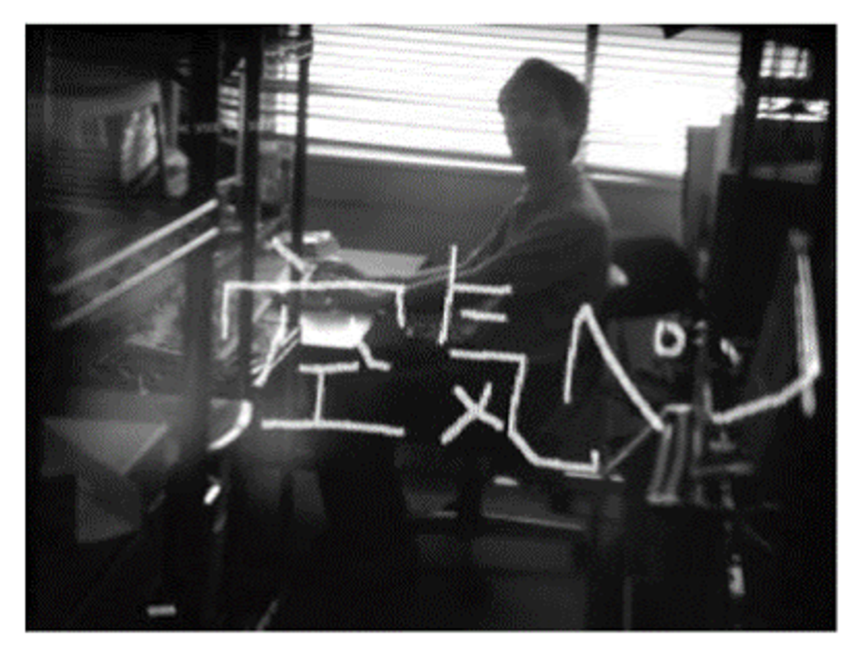
\includegraphics[clip,height=5.0cm,width=6.0cm]{./tegakijouhou.eps}
    \caption{描いた情報}
    \label{fig:tegakijouhou}
  \end{center}
\end{figure}

\begin{figure}[H]
  \begin{center}
    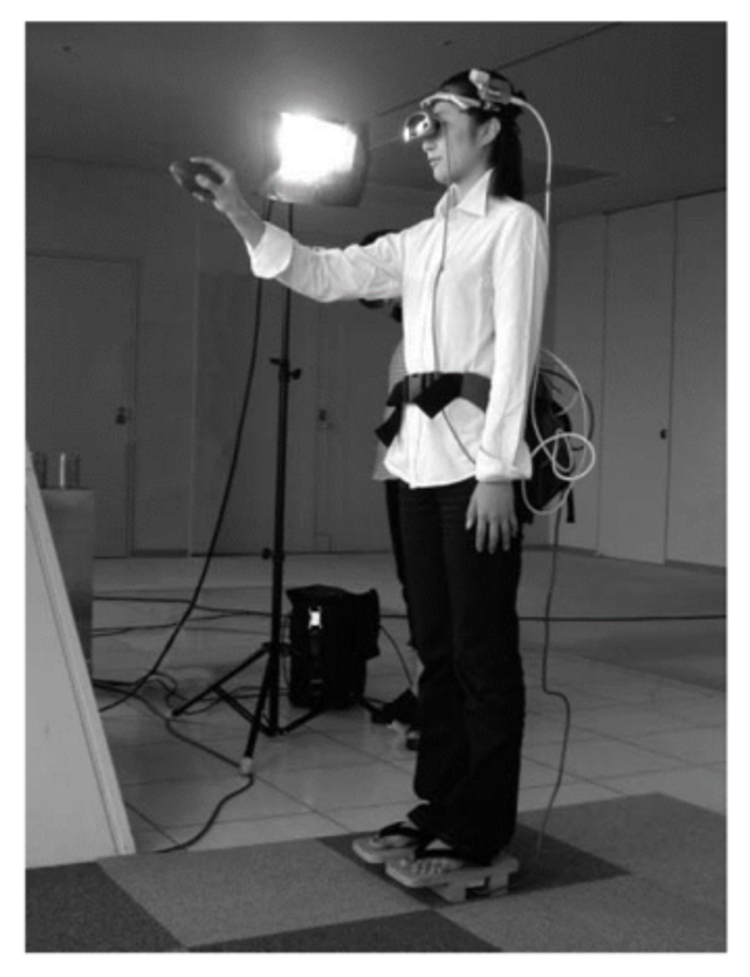
\includegraphics[clip,height=7.0cm,width=6.0cm]{./kuukipen.eps}
    \caption{空気ペン}
    \label{fig:kuukipen}
  \end{center}
\end{figure}

Agrawalら\cite{agrawal}は携帯電話が内蔵している加速度計を使用して人間の筆跡を認識するPhonePoint Penというシステムを開発した(図\ref{fig:phonepointpen})。手のジェスチャによる加速度は、幾何学的なストロークに変換されて、文字として認識される。携帯電話をペンのように持って描くことで、ユーザーは短いメッセージを書くことができ、簡単な図形を空中に描くことが可能になった。プロトタイプの評価実験を行った結果より英語の文字を平均91.9\%の精度で識別できることがわかった。

\begin{figure}[H]
  \begin{center}
    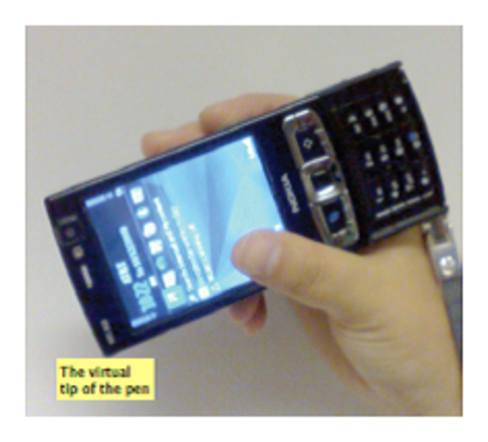
\includegraphics[clip,height=5.0cm,width=6.0cm]{./phonepointpen.eps}
    \caption{PhonePoint Pen}
    \label{fig:phonepointpen}
  \end{center}
\end{figure}

また、近年の研究ではSunら\cite{sun}は携帯端末からのWi-Fi信号を利用してハンズフリーでの描画を可能にするWiDrawを作成した。従来の研究では、ユーザーがワイヤレストランスミッタを保持する必要があるか、カスタムワイヤレスハードウェアを必要とするか、事前定義されたハンドジェスチャのみを決定する必要があったが、この研究ではウェアラブルデバイスを必要としない、W-iFiカードを使用した初めてのモーショントラッキングシステムを開発した(図\ref{fig:widraw})。

\begin{figure}[H]
  \begin{center}
    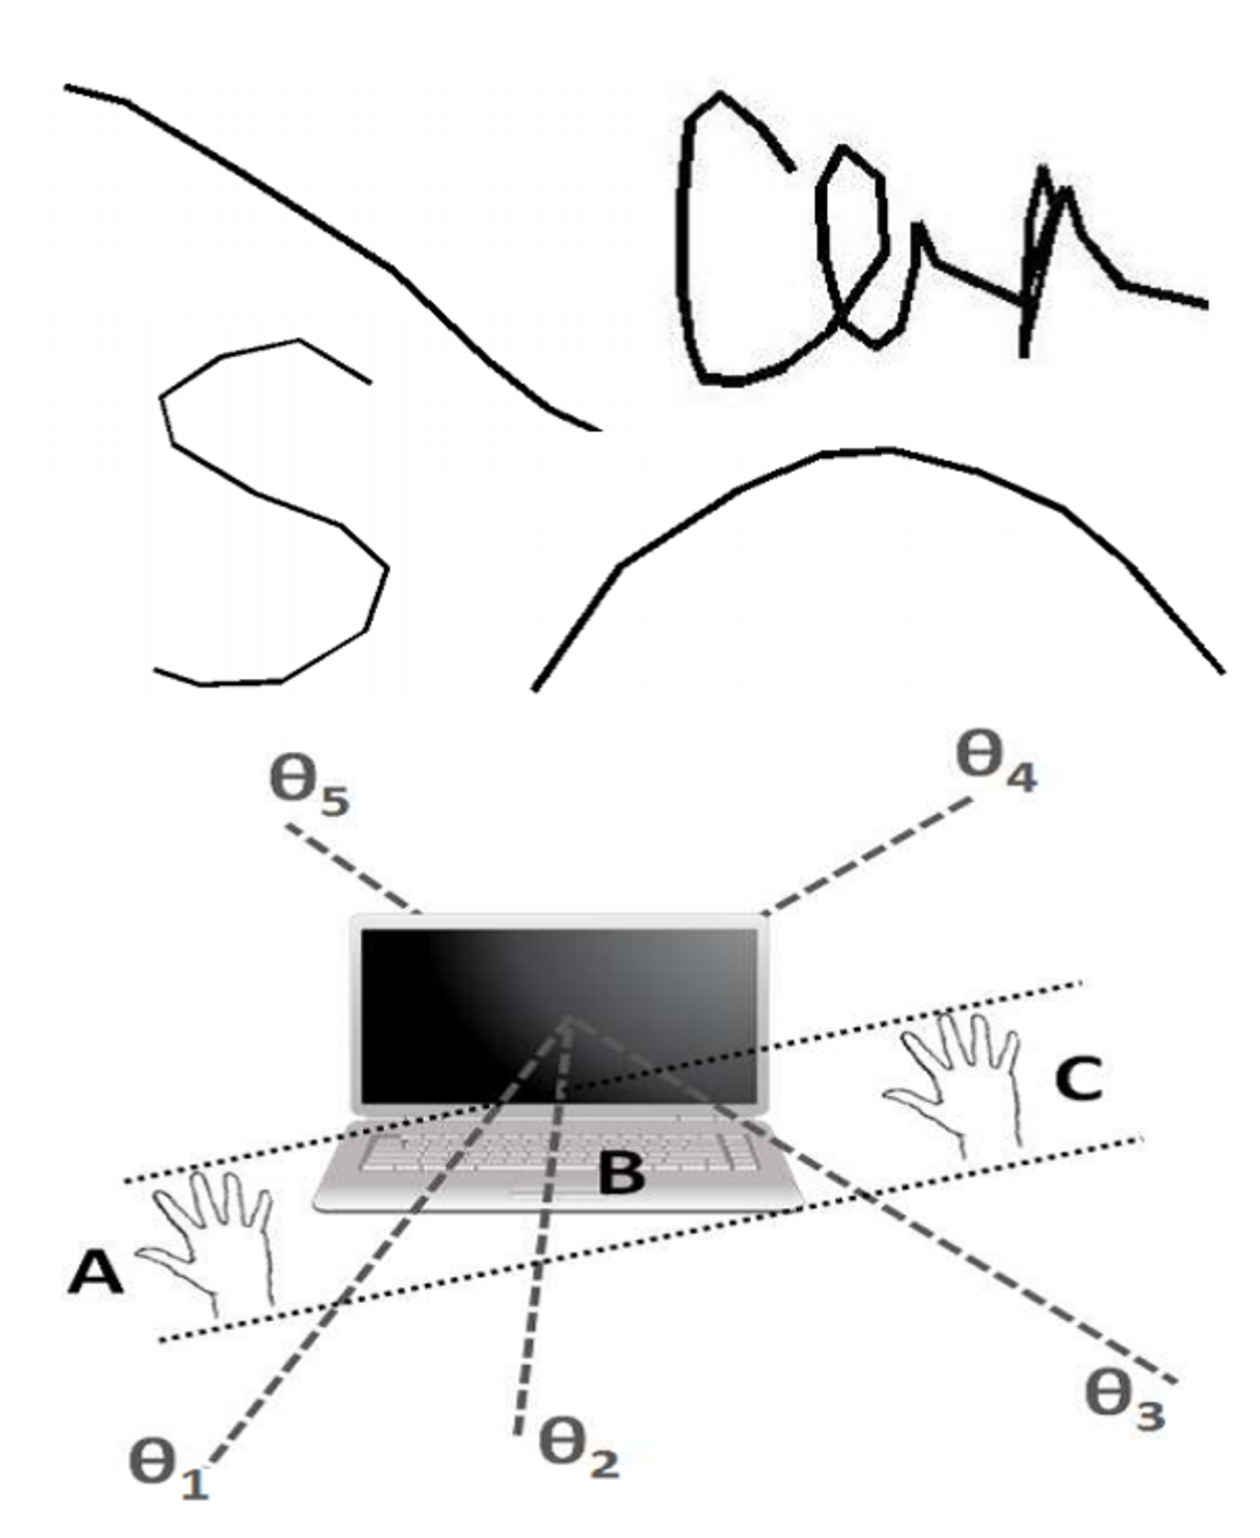
\includegraphics[clip,height=7.0cm,width=6.0cm]{./widraw.eps}
    \caption{WiDraw}
    \label{fig:widraw}
  \end{center}
\end{figure}


\subsubsection{実世界の物に関連付けてアイデアを残す研究}
高山ら\cite{tano},\cite{tano2}は実世界のどのような時間・場所であっても、ユーザが思い浮かんだふとしたアイデアを、生起を誘発したコンテキストに対応付けて保存し、それを他のユーザと共有できるシステムを作成した(図\ref{fig:informal}, \ref{fig:informal2})。ユーザーは同じような状況の時にコンテキストに対応づけて保存したインフォーマル情報を見ることができるようになった。多くのユーザーが思い浮かんだインフォーマル情報を保存することによって、実世界自体が巨大な掲示板のようになり、これによってユーザは状況に合った質の良い情報を得ることが可能になった。

\begin{figure}[H]
  \begin{center}
    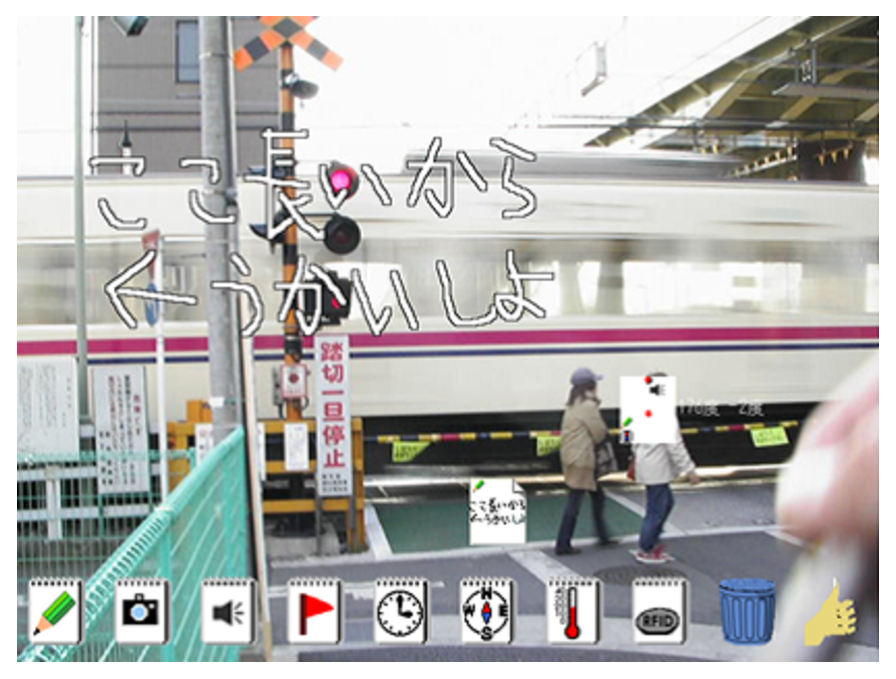
\includegraphics[clip,height=5.0cm,width=6.0cm]{./informal.eps}
    \caption{実世界の場所に関連付けてアイデアを保存}
    \label{fig:informal}
  \end{center}
\end{figure}

\begin{figure}[H]
  \begin{center}
    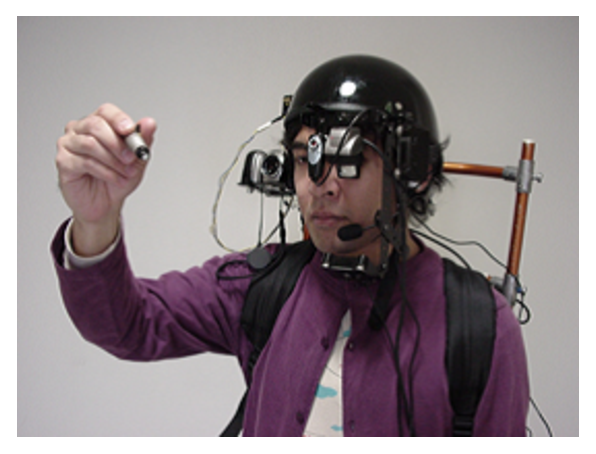
\includegraphics[clip,height=5.0cm,width=7.0cm]{./informal2.eps}
    \caption{機器を装着してるときの様子}
    \label{fig:informal2}
  \end{center}
\end{figure}

近年の研究では吉野ら\cite{yoshino}は実世界の物と関連付けたアイデアの共有による発想支援システム「ものぴこん」の開発をした。創造能力低下の原因として、日常生活における継続的な創造的思考の機会の減少が挙げられていた。この研究では、人は実空間上の「もの」を見ることで視覚刺激を受け、新しいアイデアを発想できるということに着目した。そこで、特定物体認識技術を用いることで、身の周りの「もの」を介してアイデアを日常的に共有するシステム「ものぴこん」の開発を行った(図\ref{fig:monopikon})。

\begin{figure}[H]
  \begin{center}
    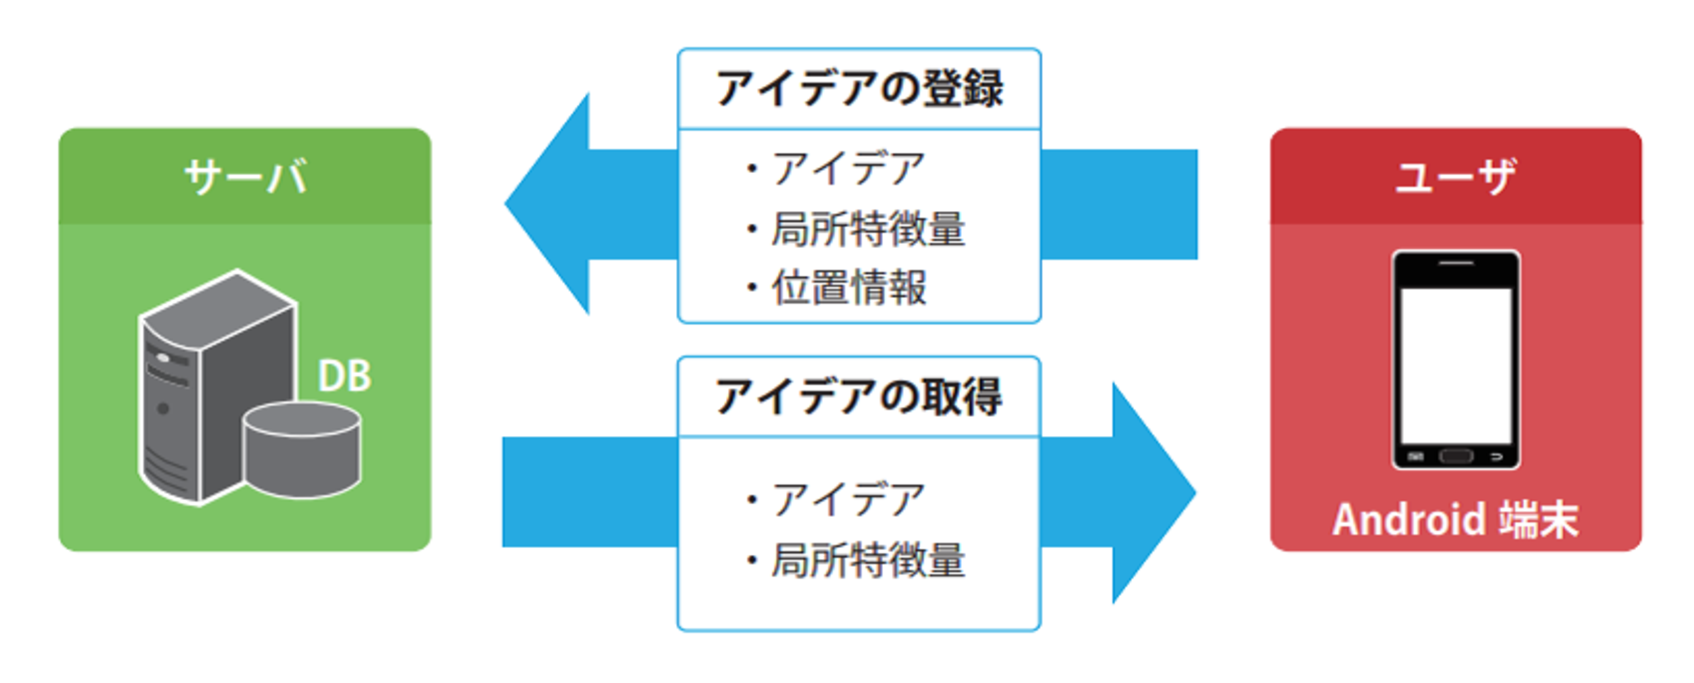
\includegraphics[clip,height=4.0cm,width=8.0cm]{./monopikon.eps}
    \caption{ものぴこんのシステム構成}
    \label{fig:monopikon}
  \end{center}
\end{figure}

\subsubsection{複数人で使用することを想定したシステムを開発する研究}
Bast\'ea-Forteら\cite{bastea}は共有キャンバスを用いてブレインストーミングを支援する共同スケッチシステムを開発した(図\ref{fig:collaborative_sketch})。共有スケッチの閾値を下げることですべてのメンバーからのアイデアの生成が増えて、他のメンバーのアイデアを構築できると考えてこのシステムを開発した。このシステムを利用することで、デジタルホワイトボードを用いた共有キャンバス上で各ユーザがタブレットPCで描写したスケッチの共有が可能になった。

\begin{figure}[H]
  \begin{center}
    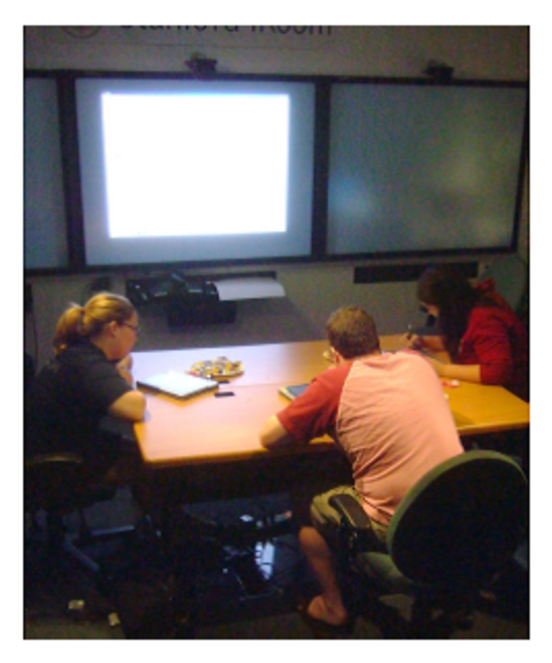
\includegraphics[clip,height=7.0cm,width=6.0cm]{./collaborative_sketch.eps}
    \caption{共同スケッチシステム}
    \label{fig:collaborative_sketch}
  \end{center}
\end{figure}

友広ら\cite{tomohiro}はタブレットPCとデプス(depth)カメラを用いてプロトタイプのスケッチインタフェースを開発した(図\ref{fig:3dsketch})。スケッチは情報記録、共有、そしてアイデアの発想のためのツールとして使用されている。2Dのスケッチを描くことと同様に3Dのスケッチが描くことが可能になれば、裏面の凹凸情報を複数視点から描かなくても状況の理解が促すことができると考えてこのシステムを作成した。

\begin{figure}[H]
  \begin{center}
    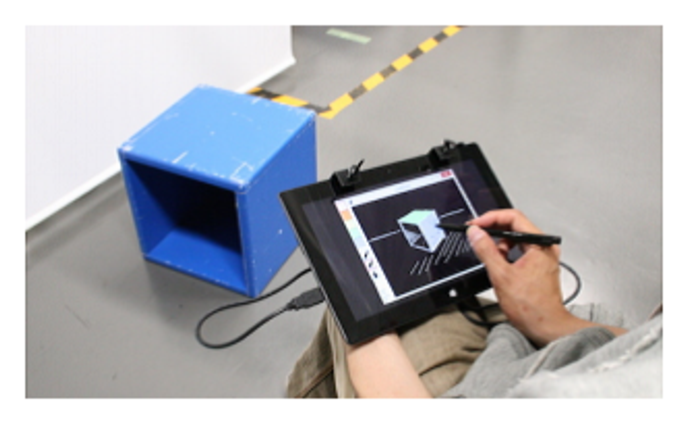
\includegraphics[clip,height=5.0cm,width=8.0cm]{./3dsketch.eps}
    \caption{3Dスケッチインタフェース}
    \label{fig:3dsketch}
  \end{center}
\end{figure}

長田ら\cite{nagata}はスマートグラスを用いた仮想空間への手書き情報共有システムを開発した(図\ref{fig:kasoukuukan})。ジェスチャの認識を用いて指の追跡を行い、軌跡を描くことで手書き情報を実現した。空間への描画は物体の動きをカメラで捉え行う。これによって仮想空間において手書き情報を共有することができるようになった。

\begin{figure}[H]
  \begin{center}
    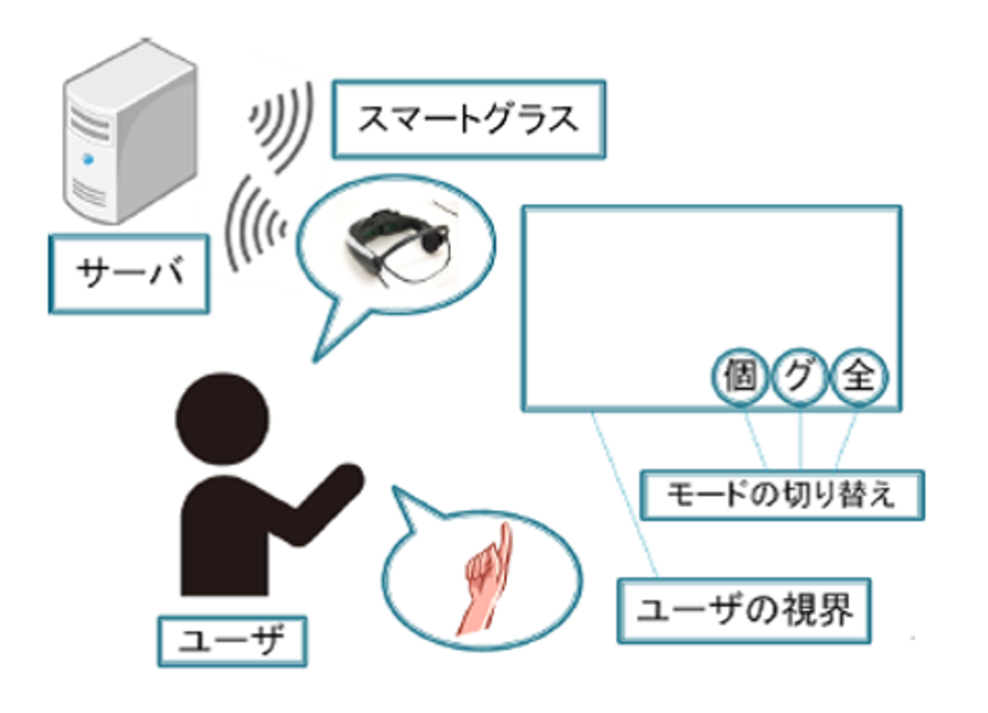
\includegraphics[clip,height=5.0cm,width=7.0cm]{./kasoukuukan.eps}
    \caption{仮想空間への情報共有システム}
    \label{fig:kasoukuukan}
  \end{center}
\end{figure}

\subsection{従来研究の問題点}
従来研究の分析を行い、以下の三つの問題点にまとめる。

\subsection*{問題点1: 同時に複数人で使用することを想定していない}
既存の研究の多くは一人で使用することを想定している。または、将来的には複数人で使用することを目標として開発を目指したが、現状では一人でしか使えない、同時に複数人では使うことができない等のシステムが多い。アイデアは一人で考えて生み出すものとは限らない。複数人で集まって話し合うことによって、一人では思いつかなかったアイデアが生まれたり、話が弾んでいくうちに連鎖的にアイデアが生まれることもある。したがって、複数人で使用可能でリアルタイムで同時に使用できるシステムが望ましい。

\subsection*{問題点2:使用できる場所が限定されている}
既存の研究の多くは特定の場所において使用することを想定している。または、持ち運びは一応可能であるが、多くの機器を装着しなければならない等のシステムで、実際に使用するのは厳しいというものが多い。アイデアはふとしたときに思い浮かぶものであり、座って作業しているときだけに限らず、歩いているときや机やホワイトボード等がないような場面でも突然思い浮かぶことがある。アイデアは思い浮かんだときに忘れないようにできるだけすぐに書き留めたほうが良い。したがって、どこでも場所を選ばずに使用できるシステムが望ましい。

\subsection*{問題点3:入力手法が限定されている}
既存の研究の多くは指のみの操作しかできない等で入力手法が限定されている。または、操作が複雑で慣れるのに時間がかかる等のシステムが多い。アイデアは短い言葉でまとめるのは困難である場合もある。また、アイデアの形は様々である。アイデアは文字だけではなく図形として残す場合もあったり、または平面の形をとったり、立体的な形をとることもある。したがって、簡単な操作で直感的に様々な入力ができるシステムが望ましい。

\newpage
\section{本研究のコンセプト}
本章では、

\subsection{新しいシステムのコンセプトの提案} \label{concept}
従来研究では一人で使用をすることを想定していたり、使用できる場所が限定される、持ち運びが難しい、操作が複雑等の問題点があった。

アイデアは一人で深く考えて練ったり生み出すこともあるが、友人との話し合いをしたり、議論をしていくうちにアイデアが生まれることがある。よって複数人で使用できるシステムが必要である。

アイデアはふとしたときに突然思い浮かぶものである。現状、私達は浮かんだアイデアを紙に書き留めたり、PCを利用してメモを取っている。しかし、アイデアが思い浮かぶのは座って作業しているときだけとは限らない。外で歩いているときや、机やホワイトボード等がないような場面でも突然思い浮かぶことがある。したがって、場所を限定することなく、どこでも使用できるシステムが必要である。

思い浮かんだアイデアは短い言葉だけで表すことが難しい場合もある。また、話した内容もそのまま残しておきたい場合もある。また、人によって入力のしやすい方法は異なる。よって、複雑なジェスチャをすることなく直感的に様々な入力ができるようなシステムが必要である。

そこで、本研究は以下の三つを満たすようなシステムを提案する(図\ref{fig:concept})。

\begin{enumerate}[(1)]
 \item 複数人で同時に使用することが可能
 \item どこでも場所を選ばず利用が可能
 \item 簡単な操作で直感的で様々な入力が可能
\end{enumerate}

それぞれについて以下に詳しく述べる。

\begin{figure}[H]
  \begin{center}
    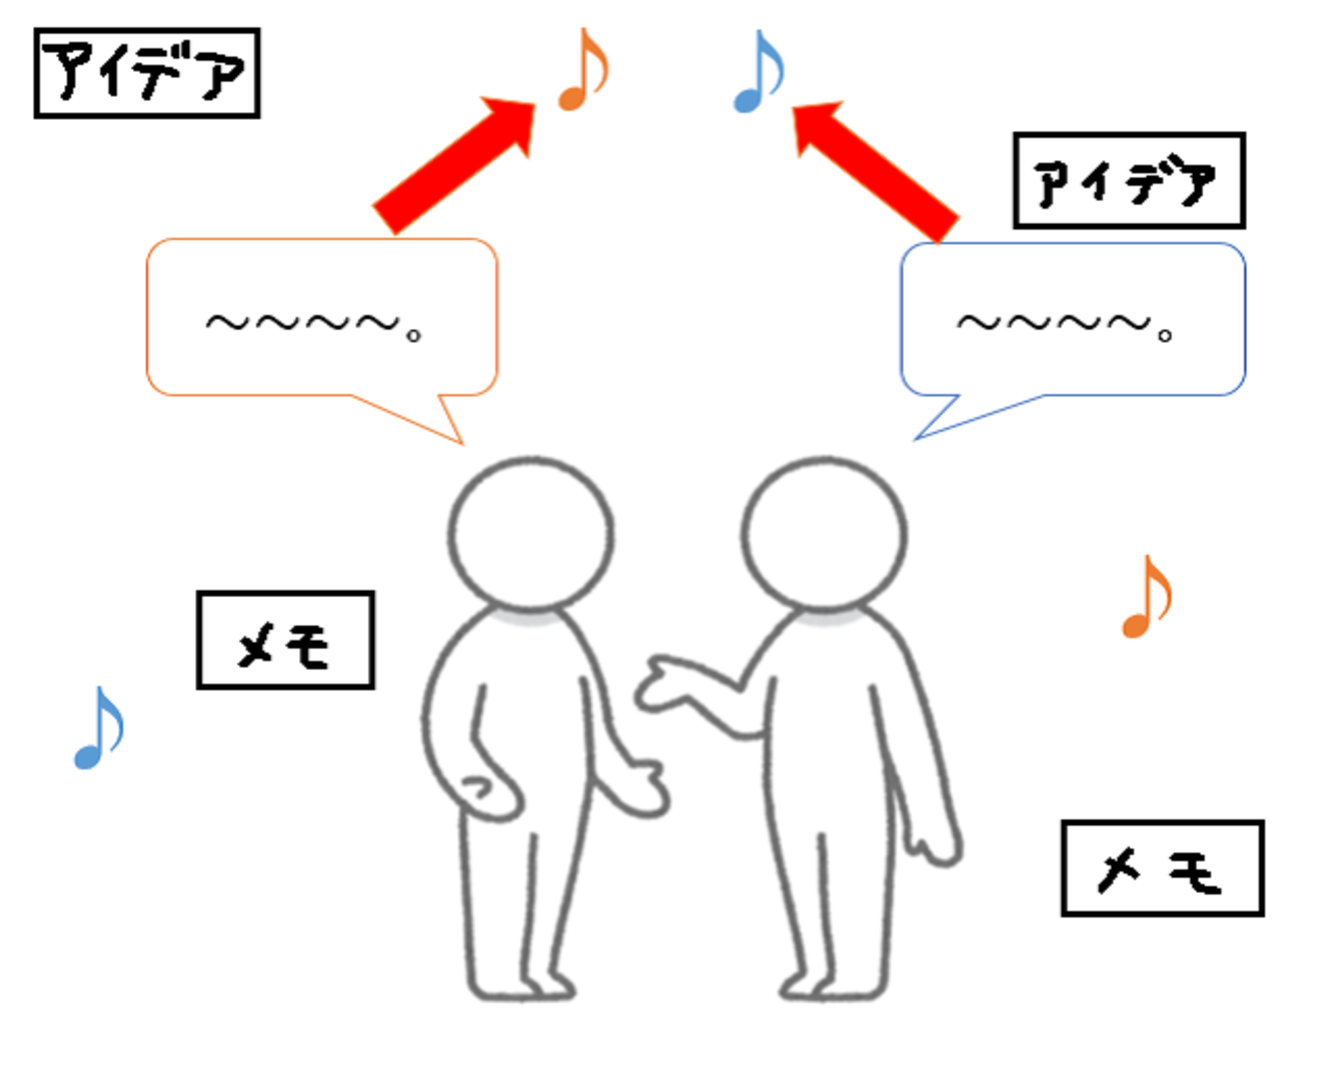
\includegraphics[clip,height=6.0cm,width=7.0cm]{./concept.eps}
    \caption{本研究のコンセプト}
    \label{fig:concept}
  \end{center}
\end{figure}

\subsection*{特徴1:複数人で同時に使用することが可能}
既存の研究では一人で使用することを想定したシステムが多かった。または、将来的には複数人で使用できるようにすることを目標にしてるが現状のシステムでは一人でしか使用できないというものも多かった。他には、複数人で使用することはできるが同時に使用することができないというものあった。アイデアは一人で考えて生み出す場合もあるが、複数人で集まって話し合って一緒に考えることによってアイデアが生まれることもある。ある人がアイデアを出せば、そのアイデアに対して他の人が反応して新たな意見を出して、そこからまた新しいアイデアが生まれることもある。それが連鎖的に続くことによって結果的にアイデアをたくさん生み出すことに繋がる。アイデアを効率的に生み出す方法が既に何種類も存在するが、その中には実際に複数人で集まって話し合ってアイデアを出し合うというものも多い。したがって、複数人で同時に使用できて、お互いのメモをリアルタイムで共有できることが必要不可欠である。また、複数人で利用する際に空間上に文字を残す場合に問題点が発生する。その問題点については\ref{moji_mondai}で詳しく述べる。

\subsection*{特徴2:どこでも場所を選ばず利用が可能}
既存の研究では机やPCの近く、または特定の場所等のみでしか使用できないシステムが多かった。他には、どこでも利用可能ではあるが多くの機器を装着しなければならなかったり等、可搬性に問題があるシステムもあった。アイデアが生まれるのは椅子に座って机で作業しているときや、黒板やホワイトボード等の前に立っているとき等、何かノート等を使ってメモを取ることができる場所だけとは限らない。アイデアは思いがけない場所でふとしたときに突然思い浮かぶことがある。時には外で歩いているときや、軽い運動をしているときに思い浮かぶこともある。実際に動きながらメモを取るのは困難である。また、普段から常にメモ帳等を持っていてすぐにメモを取る習慣がついている人は良いが、そうでない人はメモを取ることを諦めてしまったり、後回しにしまいがちである。アイデアが思い浮かんだら、当然すぐにメモを取るほうが良い。したがって、どこでも場所を選ばずに利用できるようなシステムが必要である。

\subsection*{特徴3:簡単な操作で直感的で様々な入力が可能}
既存の研究では空間上で描くのみ等で入力手法が限定されているシステムが多かった。または、特別なジェスチャを定義して使用する必要があったり、慣れるのにかなり時間がかかる等のシステムもあった。\ref{idea_katachi}でも述べるがアイデアの形は文字や図形等、様々な形をとる。立体的な形を持ったアイデアもあれば、平面の形を持ったアイデアも存在する。仮に入力手法を空間上に描くのみにした場合、考えたアイデアが短い文章にまとまらないときメモを取ることが困難である。また、仮に入力手法を音声のみにした場合、シンプルな図形であれば表示できるかもしれないが、大きさを音声入力で指定しなければならなかったり、複雑な図形を描く際は困難である。したがって、簡単な操作で直感的で様々な入力ができるシステムが必要である。

\subsection{文字を表示する上での問題点と解決案} \label{moji_mondai}
複数人で空間上に文字のメモを残す際に、見る視点によって文字として見えないという問題点が発生する。解決案として、文字を動的に相手の方向に回転させて向けたり、文字のメモに触れたら自分の前に見えるように表示する等の方法が考えられる。しかし、文字を動的に相手の方向に回転させて向けてはいけない場合もある。それは、平面上に文字のメモを残した場合である。何故ならばその平面そのものに意味があるからである。このようなメモの表示に関しての解決案は、その平面上に残した文字のメモに目線を合わせて、それ自体はそのままにしておき、その平面上に残した文字を目の前等の自分の見やすい位置に表示するという手法を提案する。

また、平面の形を持った文字以外に立体的な形を持つ文字が存在すると考えられる。立体的な文字に関してはそれ自体に意味を持つので回転したり等はしないほうがよいと考えられる。

\subsection{様々なアイデアの形} \label{idea_katachi}
アイデアの形は様々である。大きく分けると描いて残すアイデアと話して残すアイデアがあるが、それぞれのアイデアも様々な形がある。以下ではそれぞれのアイデアを細かく分けて分類した上でそれぞれについて詳しく説明する。

\subsubsection{描いて残すアイデア} \label{draw_idea}
描いて残すアイデアを細かく分けると図\ref{fig:draw_idea}のようになる。描いて残すアイデアは、最初に絵と文字に分けることができると考えられる。更に絵のアイデアは、立方体等のように空間上に線を引いて描く3Dのアイデアと、空間上に仮想的な平面を用意してそこに丸や四角形等のように平面上に線を引いて描く2Dのアイデアに分けることができると考えられる。また、文字のアイデアも同様に立体的な形を持つ3Dのアイデアと、平面上に描いて残す2Dのアイデアに分けることができると考えられる。この2Dの文字の文字に関しては実際に空間上に描いて残すには問題がある。この問題点に関しては\ref{moji_mondai}で述べたが、具体的な解決案に関しては次章で述べる。

\begin{figure}[H]
  \begin{center}
    \includegraphics[clip,height=7.0cm,width=8.0cm]{./draw_idea.eps}
    \caption{描いて残すアイデアを分類}
    \label{fig:draw_idea}
  \end{center}
\end{figure}

\subsubsection{話して残すアイデア} \label{speak_idea}
話して残すアイデアを細かく分けると図\ref{fig:speak_idea}のようになる。話して残すアイデアは、最初に絵と文字と感嘆詞に分けることができると考えられる。更に絵のアイデアは、「立方体」と発声して立方体等を出現させて残す3Dのアイデアと、「四角形」と発声して平面の形をとった四角形等を出現させて残すアイデアがあると考えられる。また、文字のアイデアは視覚的に見ることができるテキスト形式のアイデアと、議事録のように話した内容をそのままを音声として残すバイナリ形式のアイデアに分けることができると考えられる。テキスト形式の文字のアイデアは実際に空間上に話して残すには問題がある。この問題点に関しては\ref{moji_mondai}で述べたが、具体的な解決案に関しては次章で詳しく述べる。最後に感嘆詞についてであるが、人は考える際には「うーん」や「えーっと」等、思わず声に出してしまうことがある。また、声に出すことだけに限らず、頭を傾げたり、頷いたりすることもある。これらは一人で考える際には重要ではないが、複数人で話し合ってアイデアを出すときには相手がどう考えているかがある程度わかる可能性があると考えられる。

\begin{figure}[H]
  \begin{center}
    \includegraphics[clip,height=7.0cm,width=8.0cm]{./speak_idea.eps}
    \caption{話して残すアイデアを分類}
    \label{fig:speak_idea}
  \end{center}
\end{figure}

\subsection{利用シーン}
本節では\ref{concept}で述べたコンセプトを基にした提案システムの利用シナリオについて述べる。

部屋や研究室等には多くの家具や機器が配置してあると思われる。仮に広い部屋で大まかに家具の配置がしたいという状況や部屋の模様替えがしたいという場合、既存のシステムでは特定の場所でしか使えなかったり、たくさんの機器を装着しなければならなかったり等、実際に使用するのは困難である。または広い部屋は一人だけで使用する可能性は低く、多くの人が使用する共用の場所だと考えられる。よって、家具の配置や部屋の模様替えをするには複数人で話し合って決めたほうがよい。既存のシステムでは一人でしか使用できない、または複数人で使用することを想定してるが同時には使用できないというものが多く、実際に複数人で話し合って部屋の配置決めをしたり模様替えをするのは難しい。

提案システムでは持ち運びが容易で広い空間のどのような場所であっても使用が可能である。例としては部屋のある場所に椅子やテーブルが配置したいという場合、大まかに線を描いて椅子やテーブルを配置することができる(図\ref{fig:isu})。他には、部屋の高い位置に時計が配置したいという場合、手元で時計を描いて、その描いたものを操作して高い位置に移動させることによって配置することができる。また、その描画して配置した家具に対して気に入らなかったり、こうしたほうが良いと思う人が他にいたとき、それに対して新たに修正を加えたり削除することができる。描画したものに対して説明や補足をする場合、短い言葉であればそのまま手で描くことも可能であり、長い言葉で手で描くことが大変な場合は音声入力を使用して簡単にメモが残すことができる。

\begin{figure}[H]
  \begin{center}
    \includegraphics[clip,height=5.0cm,width=8.0cm]{./isu.eps}
    \caption{利用シナリオ: 家具の配置や部屋の模様替え}
    \label{fig:isu}
  \end{center}
\end{figure}

\newpage
\section{システム設計}
本章ではまず前章の\ref{concept}で述べた(1)、(2)、(3)を踏まえた上でシステムの全体構成について述べる。その次にそれぞれの機能の設計に関して詳しく説明する。また、ハードウェアは可搬性を考慮して、マイクロソフト社のHoloLens\cite{hololens}を使用する。

\subsection{全体構成}
(1)複数人で話し合って実世界の3D空間上に残したお互いのメモを共有する機能を実現するために、サーバを介して空間を共有する機能が必要である。(2)実世界の広い空間上に任意の場所にメモを置く際には、遠くにあるメモに対して操作する機能が必要である。また、(3)簡単な操作で直感的な様々な入力を可能にするには、3D空間上に描画する機能だけではなく、マルチモーダルな入力が必要となる。以上より、システムの機能としては大きく分けて、メモを入力、メモを操作、メモを共有の三つであり、以下に詳細を述べる(図\ref{fig:systemzentai})。

\begin{figure}[H]
  \begin{center}
    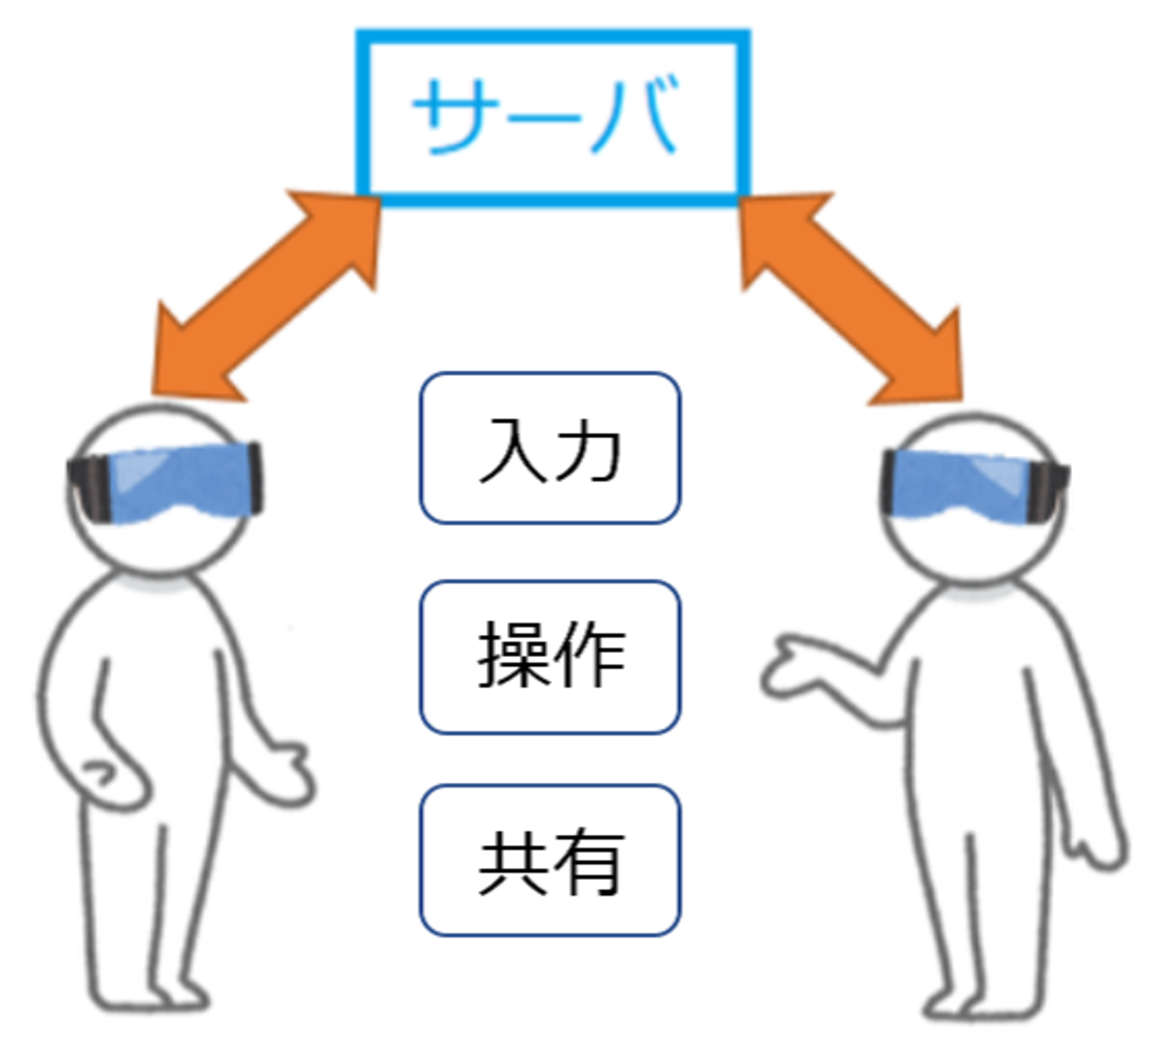
\includegraphics[clip,height=7.0cm,width=7.0cm]{./systemzentai.eps}
    \caption{システムの全体構成}
    \label{fig:systemzentai}
  \end{center}
\end{figure}

\subsection{メモを入力}

\subsubsection{描いて残すメモ} \label{draw_memo}
\ref{draw_idea}より描いて残すアイデアは、最初に絵と文字に大きく分けることができることは述べた。まず、絵のメモをどうやって残すかについて詳しく説明する。3Dの絵に関しては、タップ&ホールドを使用して空間上に線を引いて描くようにする(図\ref{fig:3d_draw})。ここで言うタップとは空間上で人差し指と親指を一度つまんで離す動作のことであり、スマートフォンで言えば画面を指で一度タッチする動作のことである。ホールドは人差し指と親指をつまんだ状態を維持することである。ホールドをしている間のみ空間上に線が出るようにして、立体的な絵を描くことができるように実現する。

\begin{figure}[H]
  \begin{center}
    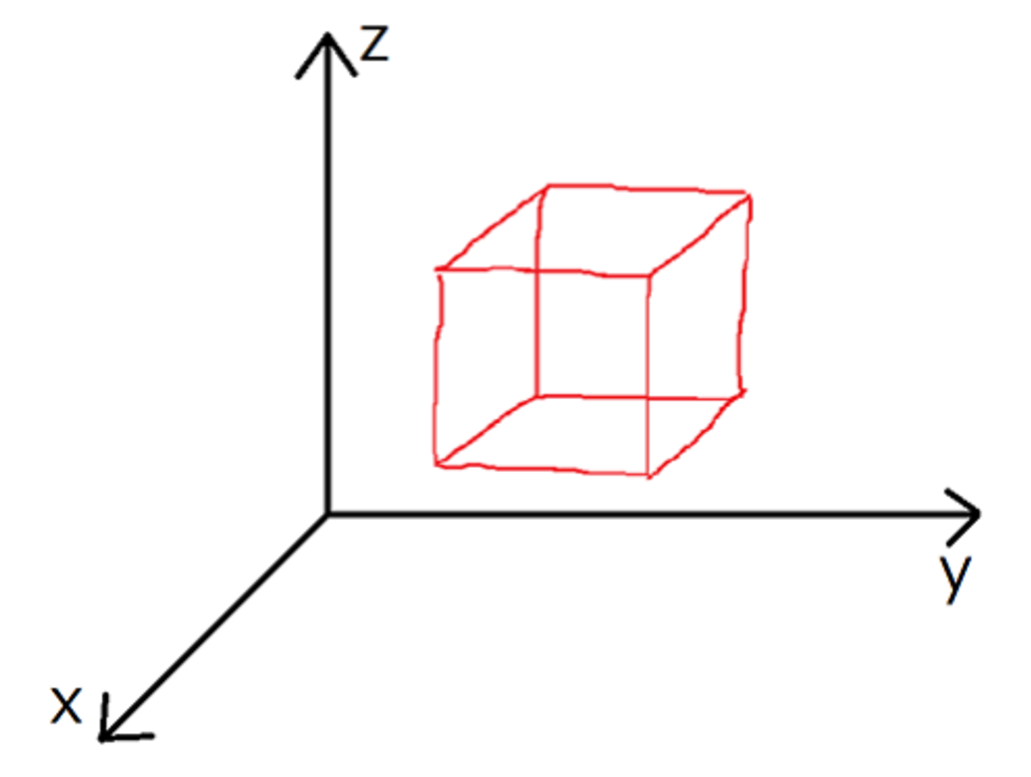
\includegraphics[clip,height=7.0cm,width=8.0cm]{./3d_draw.eps}
    \caption{3Dの絵のメモ}
    \label{fig:3d_draw}
  \end{center}
\end{figure}

2Dの絵に関しては、空間上に仮想平面を用意してその平面上に丸や四角形の図形等を描くようにする。

次に文字のメモをどうやって残すかについて説明をする。3Dの文字に関しては、3Dの絵と同様にタップ&ホールドを使用して空間上に線を引いて描くようにする(図\ref{fig:3d_moji})。

\begin{figure}[H]
  \begin{center}
    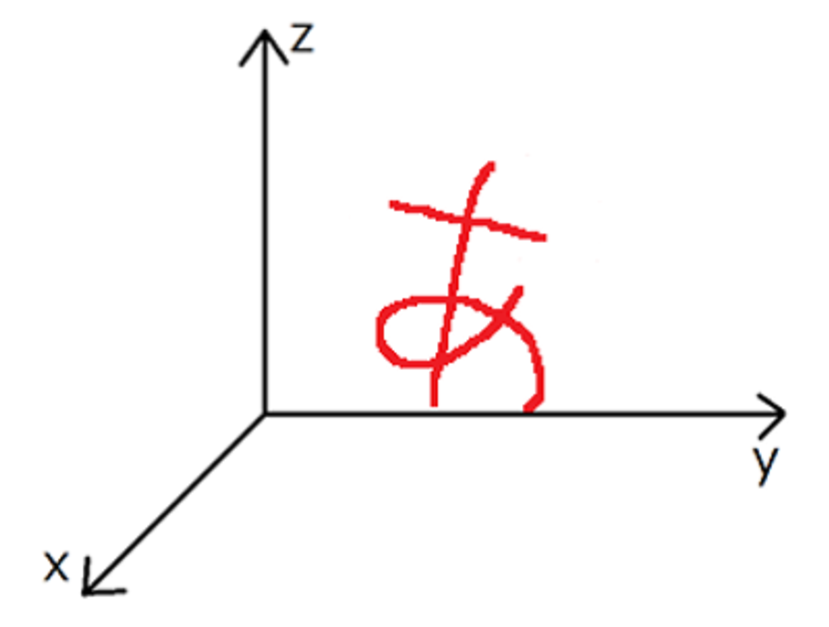
\includegraphics[clip,height=7.0cm,width=8.0cm]{./3d_moji.eps}
    \caption{3Dの文字のメモ}
    \label{fig:3d_moji}
  \end{center}
\end{figure}

2Dの文字に関しては、\ref{draw_idea}で述べたように空間上に2Dの文字を残すと見る方向によっては文字が見えないという問題が発生する。この問題の解決策としては二つ提案する。一つ目は空間上に仮想平面を用意してその平面上に文字を書き、平面ごと相手の方向に向けるという方法を提案する(図\ref{fig:memo_kaiten})。

\begin{figure}[H]
  \begin{center}
    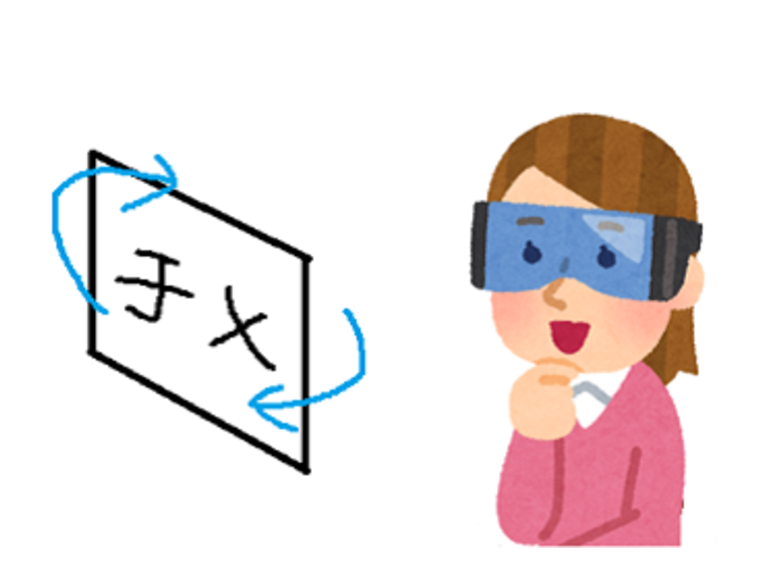
\includegraphics[clip,height=6.0cm,width=8.0cm]{./memo_kaiten.eps}
    \caption{空間上にある2Dの文字のメモは仮想平面ごと回転}
    \label{fig:memo_kaiten}
  \end{center}
\end{figure}

二つ目は描いた内容を点の情報として残すという方法を提案する(図\ref{fig:memo_ten})。閲覧する際には点をタップすることによってメモの内容を目の前に表示する。

\begin{figure}[H]
  \begin{center}
    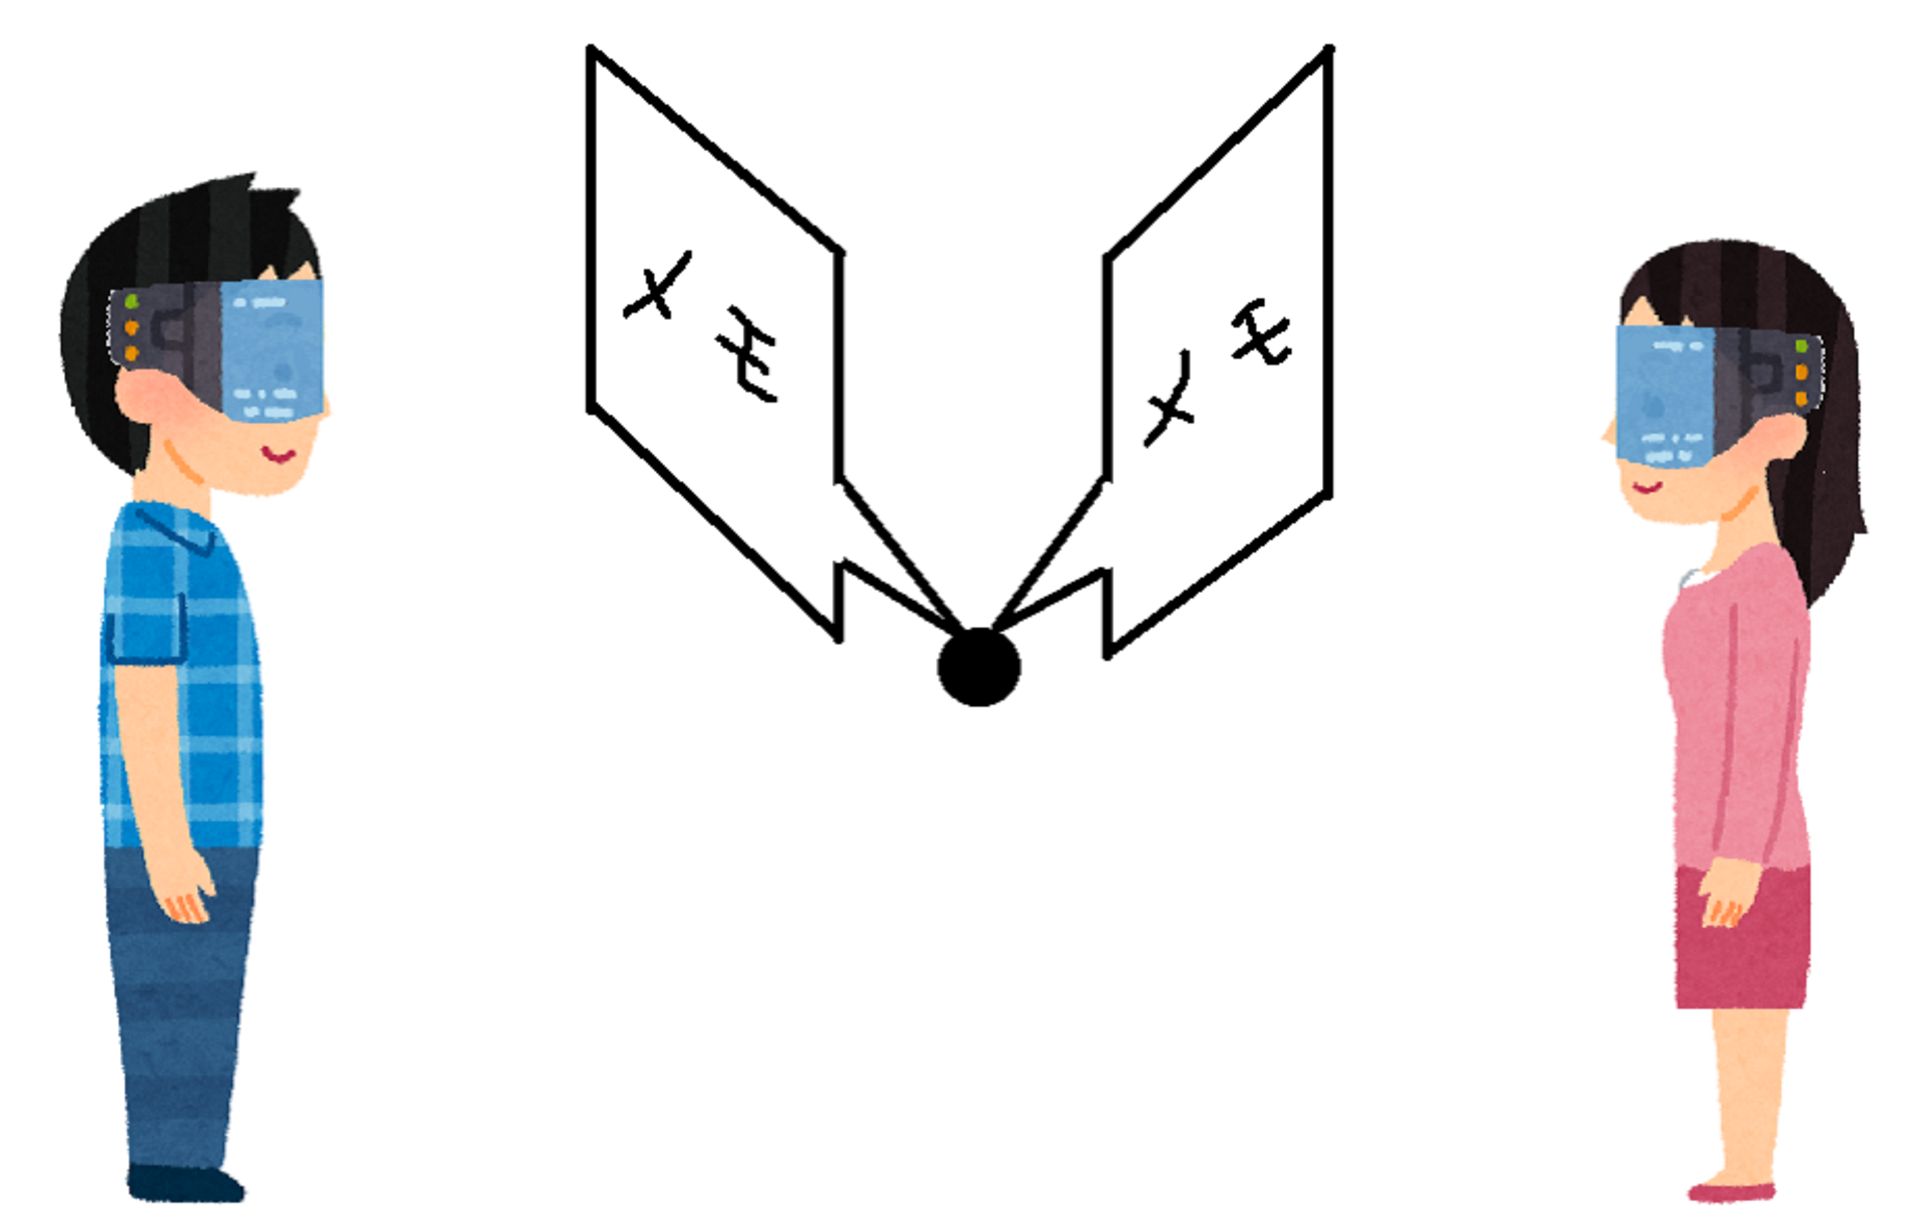
\includegraphics[clip,height=6.0cm,width=10.0cm]{./memo_ten.eps}
    \caption{点の情報として空間上に残す}
    \label{fig:memo_ten}
  \end{center}
\end{figure}

また、壁上やテーブル上等の平面のところに2Dの文字を残した場合、どうやって表示するかという新たな問題が挙がる。先ほどの空間上に残したメモの場合なら仮想平面をそのまま回転させて相手に向ければよいが、壁等にメモを残した場合は、そのまま回転させてしまうと壁の中に文字が隠れてしまう等の問題が発生する。この問題の解決策としては、壁等に残したメモはそのままにしておき、メモの内容のみを見やすいように自分や相手の目の前に表示するという方法を提案する(図\ref{fig:memo_wall})。

\begin{figure}[H]
  \begin{center}
    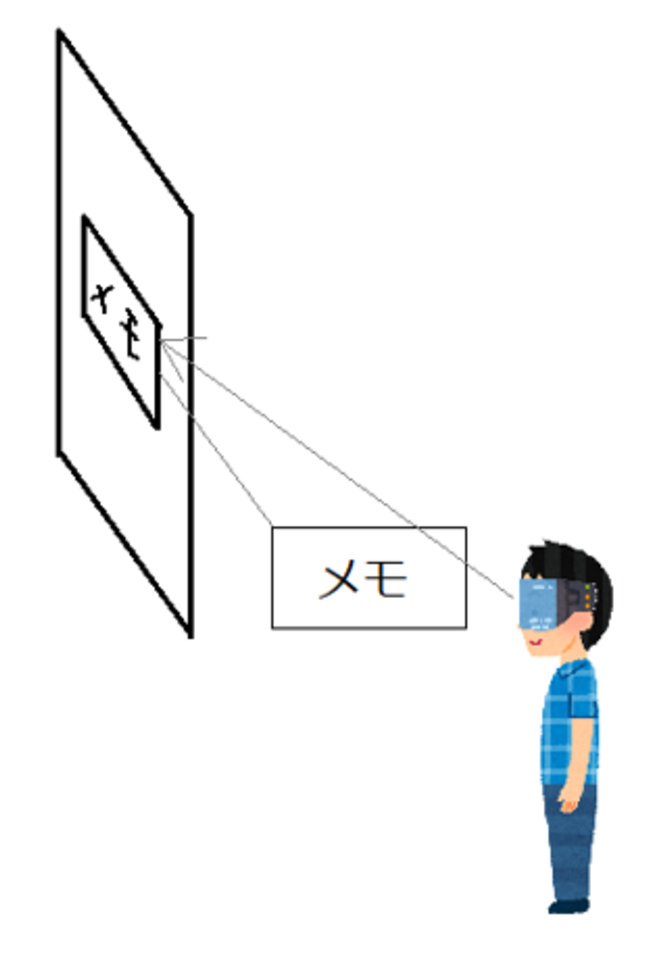
\includegraphics[clip,height=8.0cm,width=6.0cm]{./memo_wall.eps}
    \caption{壁等に残したメモは自分や相手の目の前に表示}
    \label{fig:memo_wall}
  \end{center}
\end{figure}

\subsubsection{話して残すメモ}
\ref{speak_idea}より描いて残すアイデアは、最初に絵と文字と感嘆詞に大きく分けることができることは述べた。まず、絵のメモをどうやって残すかについて詳しく説明する。3Dの絵に関しては、「立方体」等と発声することによって目の前に立体の図形を出現させる(図\ref{fig:speak_3d})。2Dの絵に関しては、仮想平面を用意した上で「丸」や「四角形」等と発声することによって平面上に図形を出現させる。

\begin{figure}[H]
  \begin{center}
    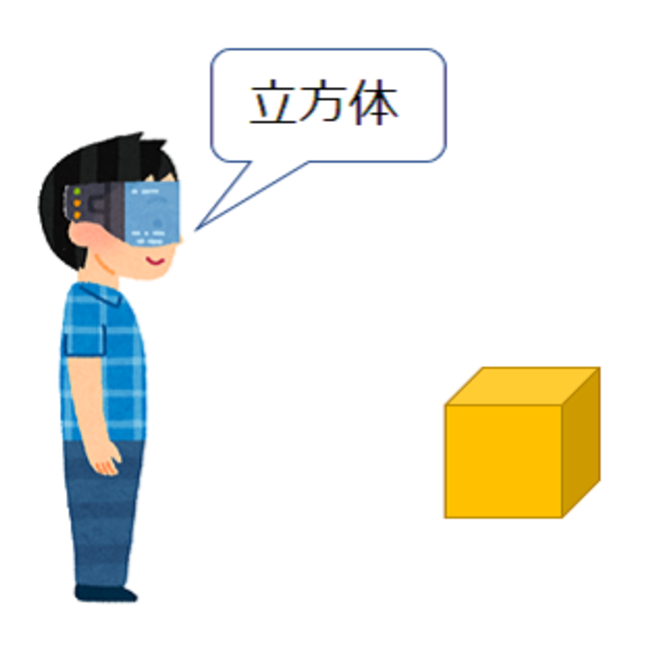
\includegraphics[clip,height=7.0cm,width=8.0cm]{./speak_3d.eps}
    \caption{発声して3Dの図形を表示}
    \label{fig:speak_3d}
  \end{center}
\end{figure}

次に文字のメモをどうやって残すかについて説明をする。テキスト形式のメモに関してはここでは二つ提案する。一つ目は空間上に仮想平面を用意し、その平面上に話した内容を文字として表示する(図\ref{fig:text_memo})。文字の向きの問題については、\ref{draw_memo}で述べた方法と同様の方法を使用して解決をする。

\begin{figure}[H]
  \begin{center}
    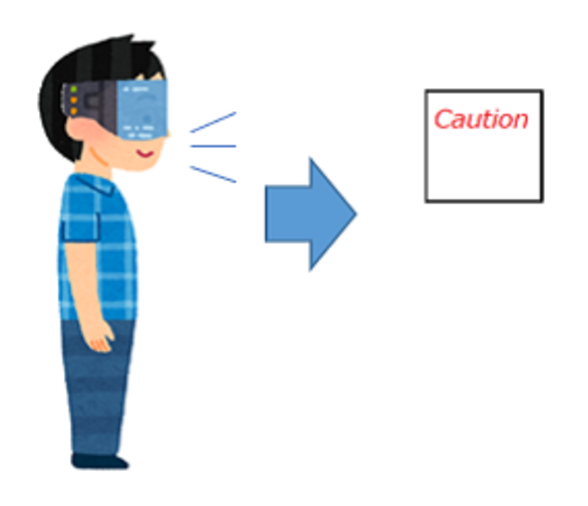
\includegraphics[clip,height=6.0cm,width=7.0cm]{./text_memo.eps}
    \caption{仮想平面を用意してその平面上に話した内容を文字化}
    \label{fig:text_memo}
  \end{center}
\end{figure}

二つ目は話しながら空間上でタップ&ホールドをして線を引き、話した内容をその線上に文字として表示する(図\ref{fig:text_memo2})。

\begin{figure}[H]
  \begin{center}
    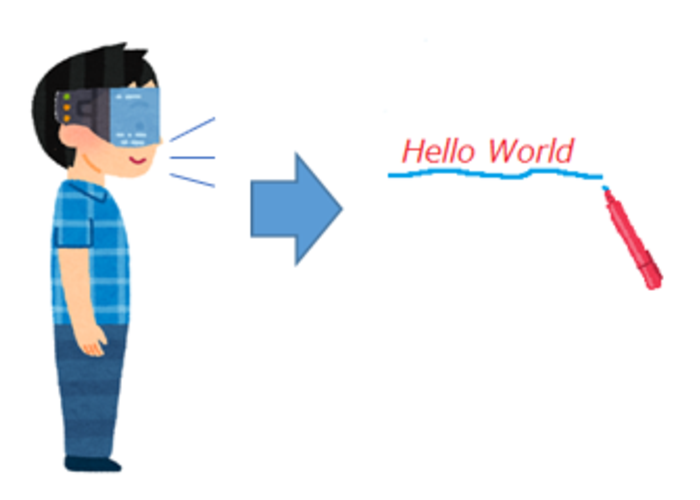
\includegraphics[clip,height=6.0cm,width=8.0cm]{./text_memo2.eps}
    \caption{話しながら線を引いて線上に話した内容を文字化}
    \label{fig:text_memo2}
  \end{center}
\end{figure}

ここで円や曲がった部分に線を引いて線上に文字を残す場合、どうやって表示するかという問題が挙がる。文字を動的に自分または相手の方向にすべて向けてしまうと図\ref{fig:moji_douteki}のようになり、かなり見づらくなってしまう。

\begin{figure}[H]
  \begin{center}
    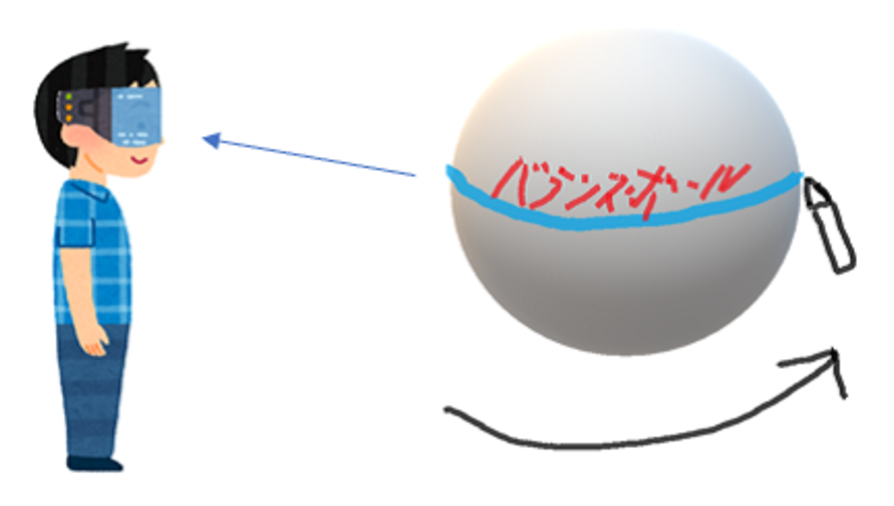
\includegraphics[clip,height=6.0cm,width=10.0cm]{./moji_douteki.eps}
    \caption{動的に文字を回転させて表示させた場合}
    \label{fig:moji_douteki}
  \end{center}
\end{figure}

この問題の解決策として二つ提案する。一つ目はタップ&ホールドをして空間上に描くときに手をひねるようにして向きを変えて、それに合わせて文字の向きも変化させるという方法を提案する。二つ目は自分自身も動きながらタップ&ホールドをして目の前に描き、そのときの自分の方向に固定して文字を向けるという方法を提案する。例としては、円ならば外側を向くように文字を表示させるようにする(図\ref{fig:moji_seiteki})。

\begin{figure}[H]
  \begin{center}
    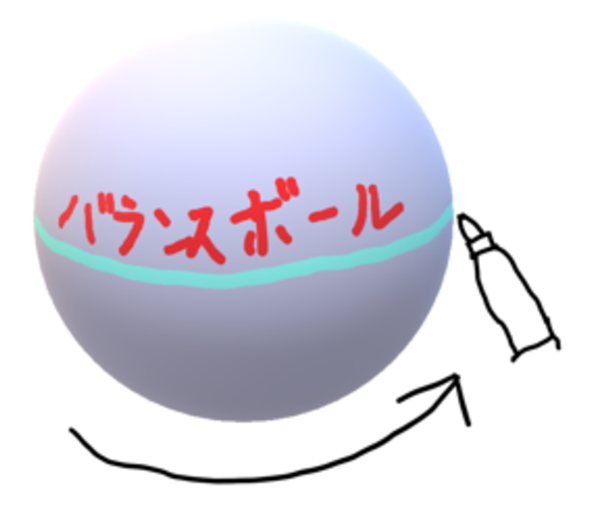
\includegraphics[clip,height=6.0cm,width=7.0cm]{./moji_seiteki.eps}
    \caption{円ならば外側に向くように文字を表示}
    \label{fig:moji_seiteki}
  \end{center}
\end{figure}

最後の感嘆詞について説明をする。「おぉ!」等と発声したときや頷く動作をした場合、その人の頭の上に「!」等を表示する方法を提案する(図\ref{fig:kantanshi})。同様に「え?」や「うーん」等と発声したときや首をゆっくりかしげる動作をした場合、「?」等を頭の上に表示する。また、一定時間発声してない場合は頭の上に「無言」や「…。」等を表示をする。

\begin{figure}[H]
  \begin{center}
    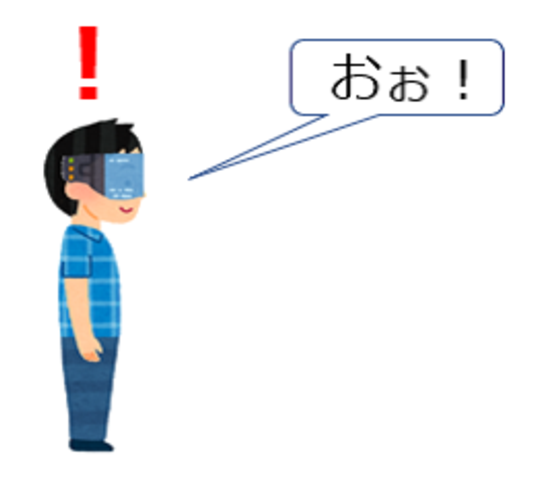
\includegraphics[clip,height=6.0cm,width=7.0cm]{./kantanshi.eps}
    \caption{頭の上に表示}
    \label{fig:kantanshi}
  \end{center}
\end{figure}

\subsection{メモを操作}
空間上に残したメモをどうやって操作するかについて、以下に近くにあるメモと遠くにあるメモに関してそれぞれ詳しく説明をする。

\subsubsection{近くにあるメモを操作}
操作に関しては大きく分けると選択、移動、削除に分けることができると考えられる。まず、メモの選択については視線を目の前にあるメモに合わせた状態で、タップをする。そして、タップ&ホールドを使用して、メモを掴んで自由に移動させる。削除に関しては、メモを選択した状態で新たに目の前に削除ボタンを用意してそれをタップするか、「削除」と発声してメモを削除する。

\subsubsection{遠くにあるメモを操作}
広い空間上でメモを操作するとき、遠くにあるメモをどうやって操作するかという問題が挙がる。ここでは以下の三つのインタラクションを提案し、それぞれについて詳しく説明する。

\begin{enumerate}[(1)]
 \item ルームスケールチェンジ
 \item 3Dラバーバンド
 \item 3Dフィッシング
\end{enumerate}

まず、(1)のルームスケールチェンジについて説明する。広い空間上で遠くにあるメモを操作したいとき、部屋全体の形状のデータと部屋内にあるメモのデータを得る。そして、図\ref{fig:room_shukusho}のように部屋全体の形状の大きさと部屋内のメモの大きさを縮小する。縮小については図\ref{fig:shukusho_temoto}のように手元にバーを用意し、バーを操作することによって大きさを変化させる。最後に、縮小したメモを手元で操作する。このようにして、遠くにあるメモを手元で操作することによって実現する。

\begin{figure}[H]
  \begin{center}
    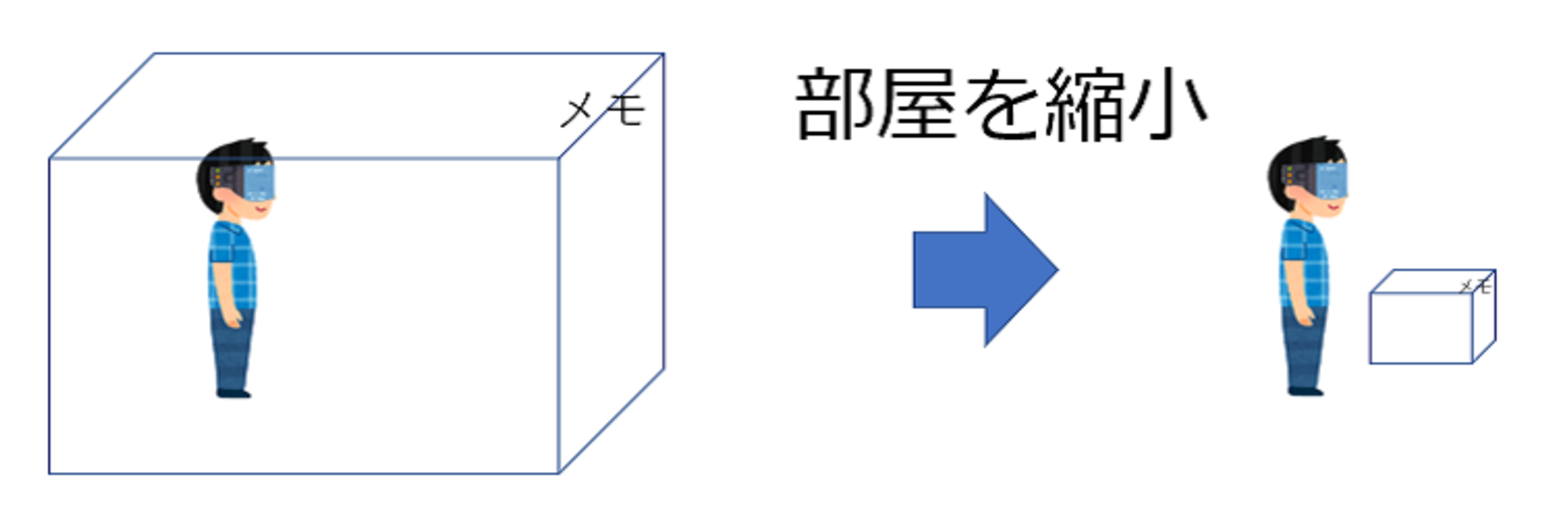
\includegraphics[clip,height=6.0cm,width=14.0cm]{./room_shukusho.eps}
    \caption{部屋全体を縮小}
    \label{fig:room_shukusho}
  \end{center}
\end{figure}

\begin{figure}[H]
  \begin{center}
    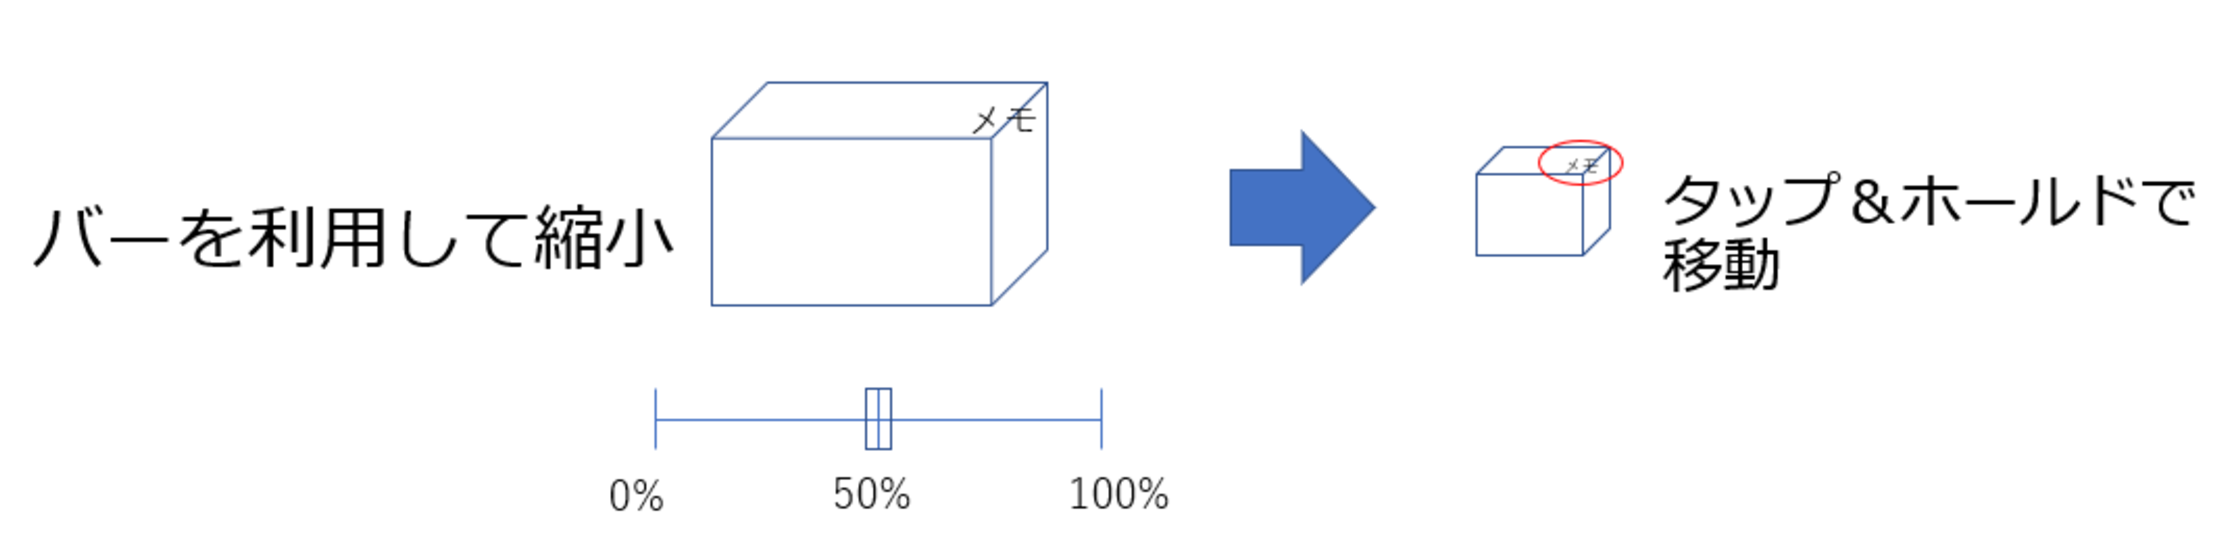
\includegraphics[clip,height=5.0cm,width=17.0cm]{./shukusho_temoto.eps}
    \caption{手元のバーを操作}
    \label{fig:shukusho_temoto}
  \end{center}
\end{figure}

次に(2)の3Dラバーバンドについて説明する。メモを選択する際は、図\ref{fig:3d_rubber_band}のように空間上に残したメモの一覧を目の前にリスト化して表示して選択を行う。空間上にあるメモとリスト内にあるメモは連動している。メモを移動する際には、目の前の移動ボタンをタップした後、図\ref{fig:3d_rubber_band2}のように手元に用意したオブジェクトを操作する。手元のオブジェクトの操作はイメージとしては輪ゴムを引っ張る感覚で引っ張り、引っ張った方向に空間上のメモも連動して移動する(図\ref{fig:3d_rubber_band3}, \ref{fig:3d_rubber_band4})。オブジェクトが中心から離れれば離れるほど移動速度が増し、オブジェクトを離すと中心に戻り、メモも停止する。削除に関してはメモを選択して削除ボタンをタップする。

\begin{figure}[H]
  \begin{center}
    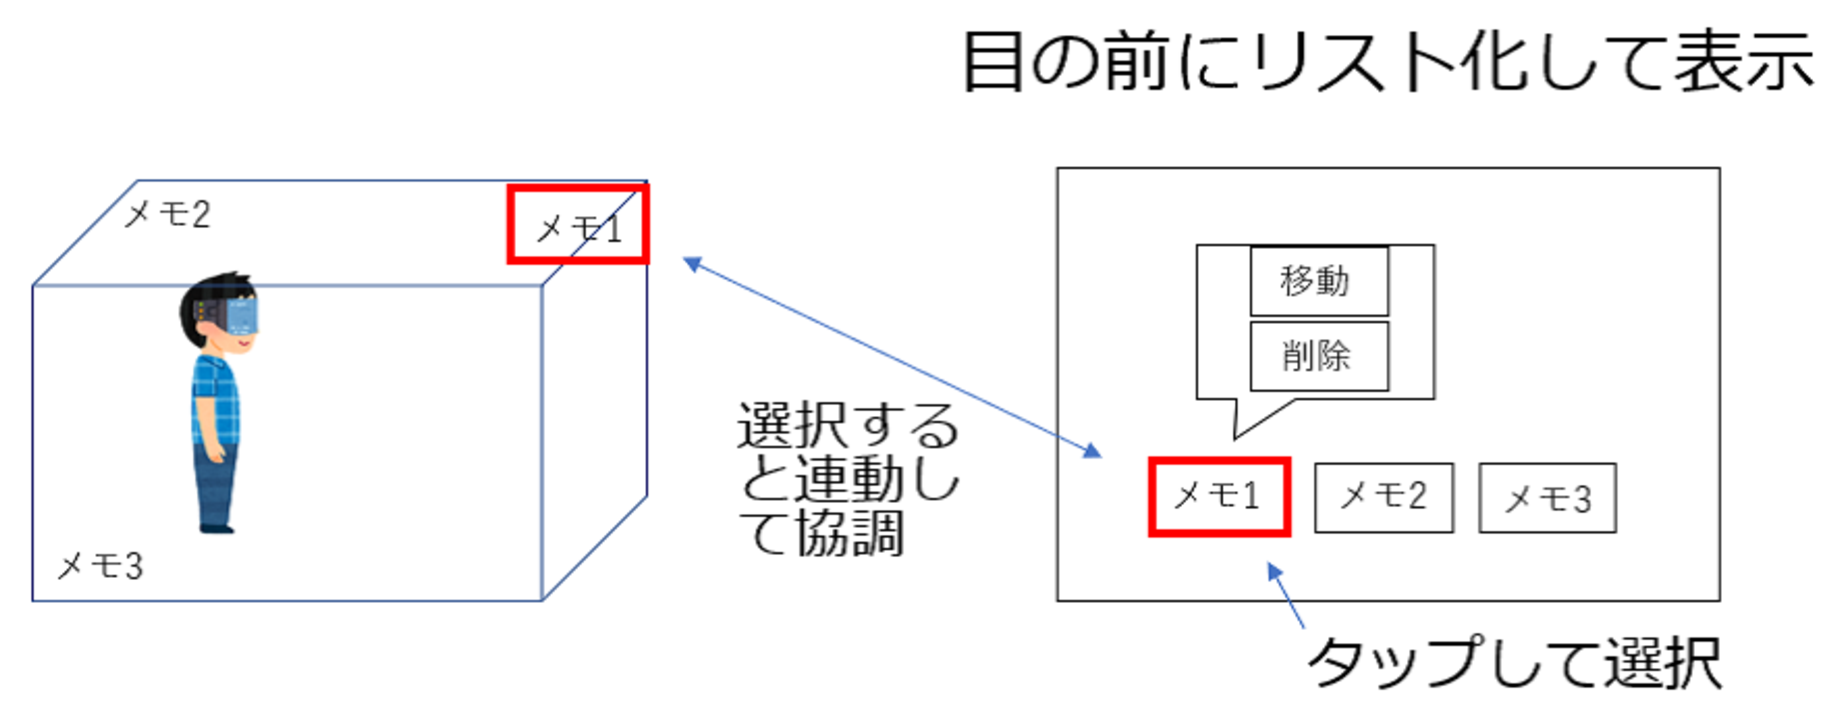
\includegraphics[clip,height=6.0cm,width=14.0cm]{./3d_rubber_band.eps}
    \caption{目の前にリスト化して表示したものを選択}
    \label{fig:3d_rubber_band}
  \end{center}
\end{figure}

\begin{figure}[H]
  \begin{center}
    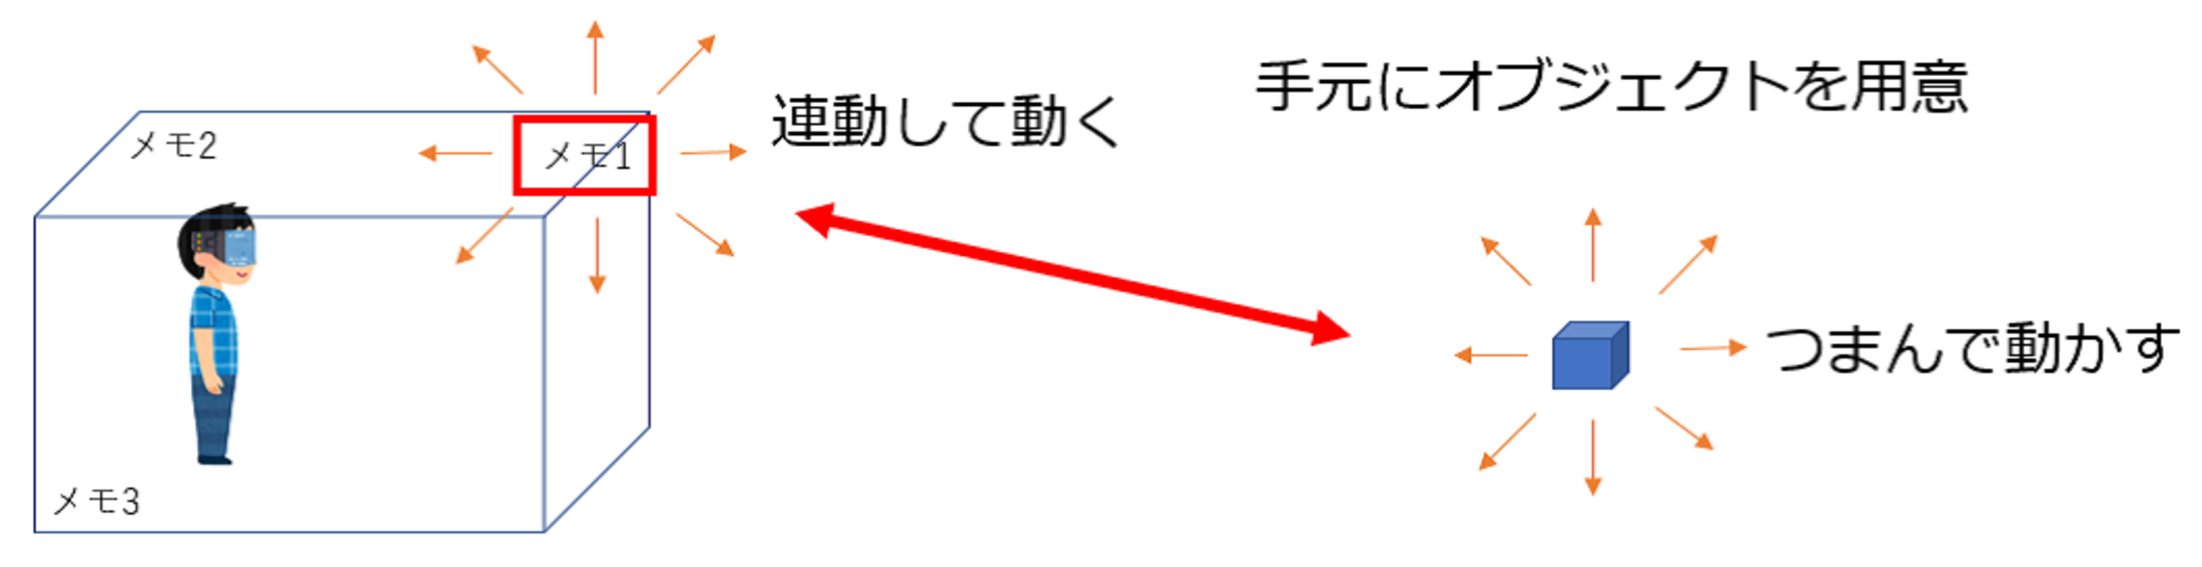
\includegraphics[clip,height=5.0cm,width=16.0cm]{./3d_rubber_band2.eps}
    \caption{手元にオブジェクトを用意}
    \label{fig:3d_rubber_band2}
  \end{center}
\end{figure}

\begin{figure}[H]
  \begin{center}
    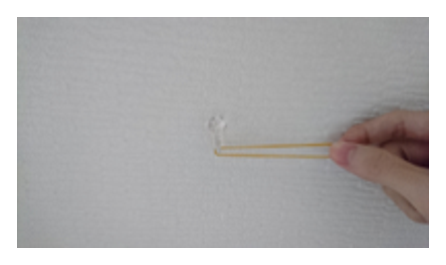
\includegraphics[clip,height=5.0cm,width=7.0cm]{./3d_rubber_band3.eps}
    \caption{操作のイメージ}
    \label{fig:3d_rubber_band3}
  \end{center}
\end{figure}

\begin{figure}[H]
  \begin{center}
    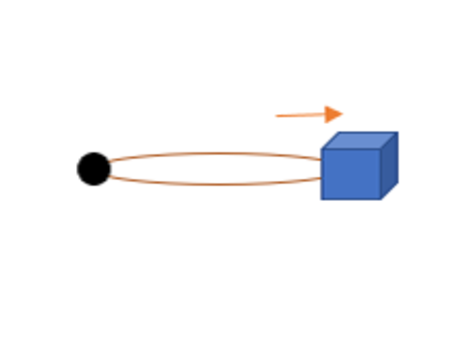
\includegraphics[clip,height=5.0cm,width=6.0cm]{./3d_rubber_band4.eps}
    \caption{手元のオブジェクトを操作}
    \label{fig:3d_rubber_band4}
  \end{center}
\end{figure}

最後に(3)の3Dフィッシングについて説明する。最初に空間上に残したメモに視線を合わせて(図\ref{fig:3d_fishing})、「選択」と発声してメモを選択する(図\ref{fig:3d_fishing2})。メモの移動については、手元にオブジェクトを用意して(図\ref{fig:3d_fishing3})、頭の動きと手元のオブジェクトの回転を利用して移動させる(図\ref{fig:3d_fishing4})。

\begin{figure}[H]
  \begin{center}
    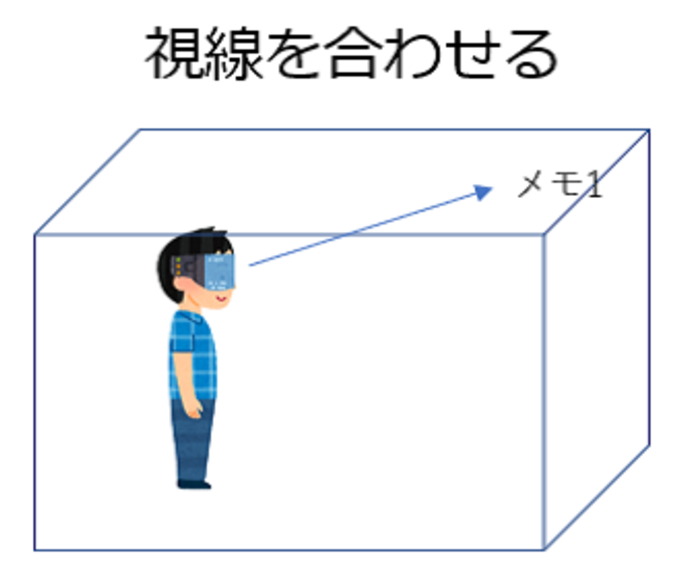
\includegraphics[clip,height=6.0cm,width=7.0cm]{./3d_fishing.eps}
    \caption{視線をメモに合わせる}
    \label{fig:3d_fishing}
  \end{center}
\end{figure}

\begin{figure}[H]
  \begin{center}
    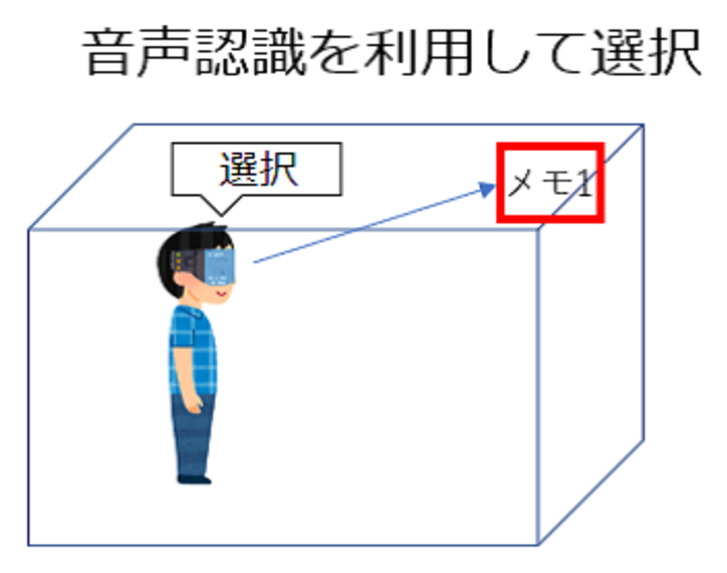
\includegraphics[clip,height=6.0cm,width=7.0cm]{./3d_fishing2.eps}
    \caption{「選択」と発声してメモを選択}
    \label{fig:3d_fishing2}
  \end{center}
\end{figure}

\begin{figure}[H]
  \begin{center}
    
\includegraphics[clip,height=4.0cm,width=7.0cm]{./3d_fishing3.eps}
    \caption{手元にオブジェクトを用意}
    \label{fig:3d_fishing3}
  \end{center}
\end{figure}

\begin{figure}[H]
  \begin{center}
    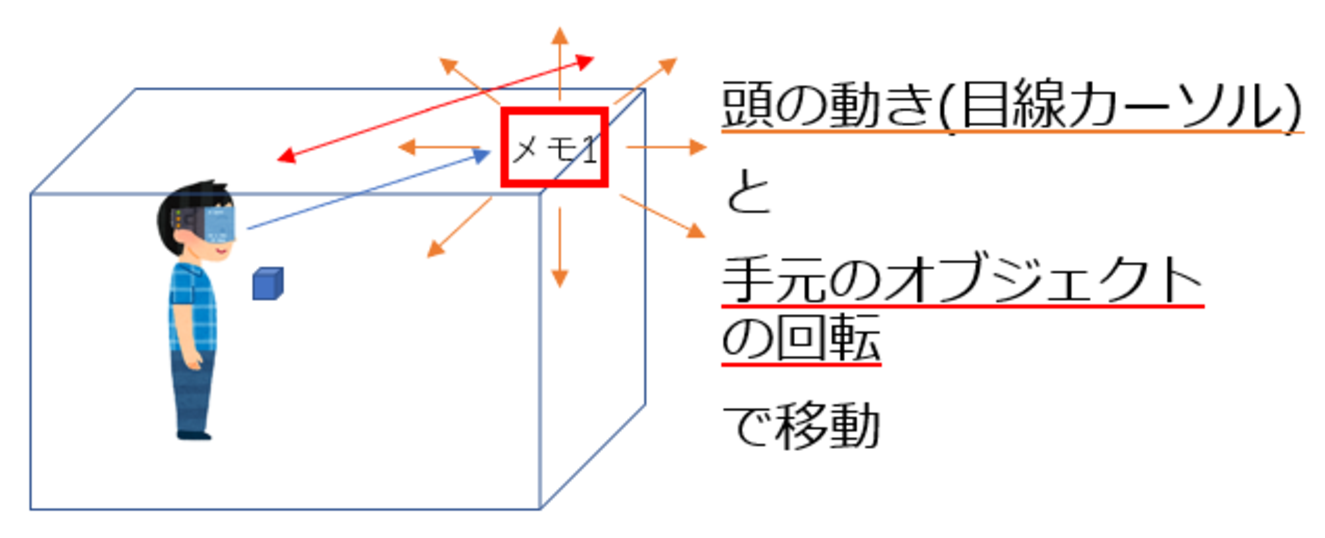
\includegraphics[clip,height=6.0cm,width=13.0cm]{./3d_fishing4.eps}
    \caption{頭の動きと手元のオブジェクトの回転を利用して移動}
    \label{fig:3d_fishing4}
  \end{center}
\end{figure}


\subsection{メモを共有}
複数人で使用するにはメモを共有できなければならない。以下には対面にいる相手と遠隔にいる相手に共有する方法をそれぞれ説明する。

\subsubsection{対面にいる相手にメモを共有}
ここでは対面にいる相手にメモを共有する方法について説明する。リアルタイムで空間上に残したメモを共有したい場合、相手側から見ても同じ場所にメモがあるように見えるように座標をサーバに送信して共有を行う(図\ref{fig:sharing_taimen})。

\begin{figure}[H]
  \begin{center}
    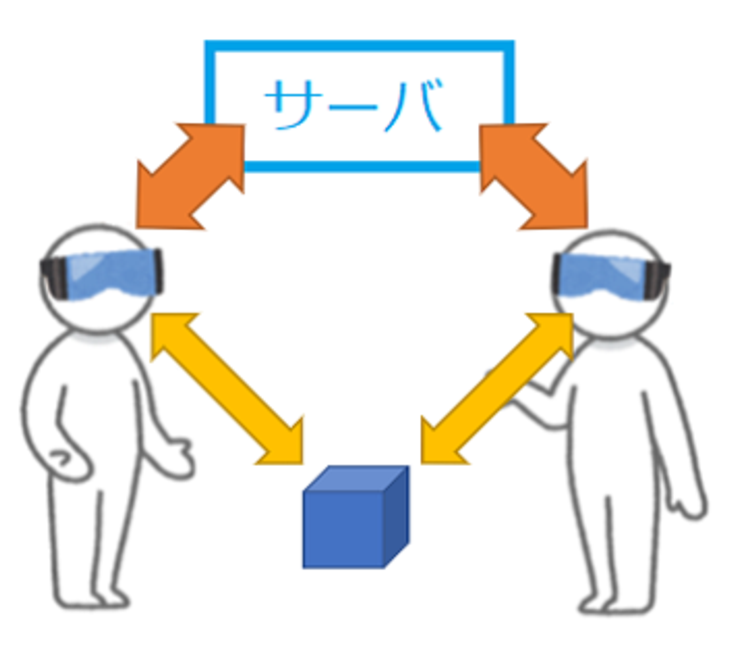
\includegraphics[clip,height=7.0cm,width=7.0cm]{./sharing_taimen.eps}
    \caption{同じ場所にメモがあるように見えるように共有}
    \label{fig:sharing_taimen}
  \end{center}
\end{figure}

また、自分が持っているメモの中で見せてもよいメモと見せたくないメモがあることを考慮して、メモはタップするまでは相手には見えないようにする(図\ref{fig:sharing_taimen2})。

\begin{figure}[H]
  \begin{center}
    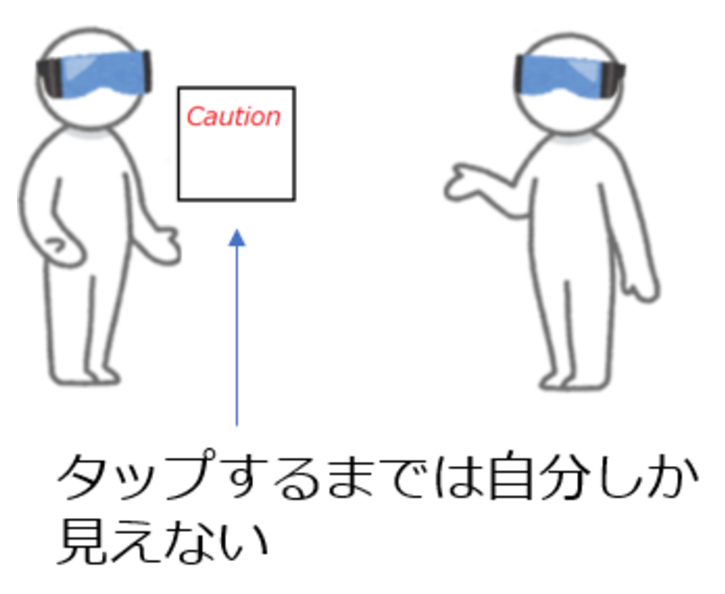
\includegraphics[clip,height=7.0cm,width=8.0cm]{./sharing_taimen2.eps}
    \caption{見せたいメモだけを共有}
    \label{fig:sharing_taimen2}
  \end{center}
\end{figure}

\subsubsection{遠隔にいる相手にメモを共有}
ここでは遠隔にいる相手にメモを共有する方法について説明する。リアルタイムでこの場所に残したメモを遠隔にいる相手にも共有したい場合があるとする。リアルタイムでメモの共有を行っている際に、遠隔にいる相手が描いたメモが突然空間に現れるという問題が発生する。そこで、遠隔にいる相手はアバターを表示するという方法を提案する(図\ref{fig:sharing_enkaku})。

\begin{figure}[H]
  \begin{center}
    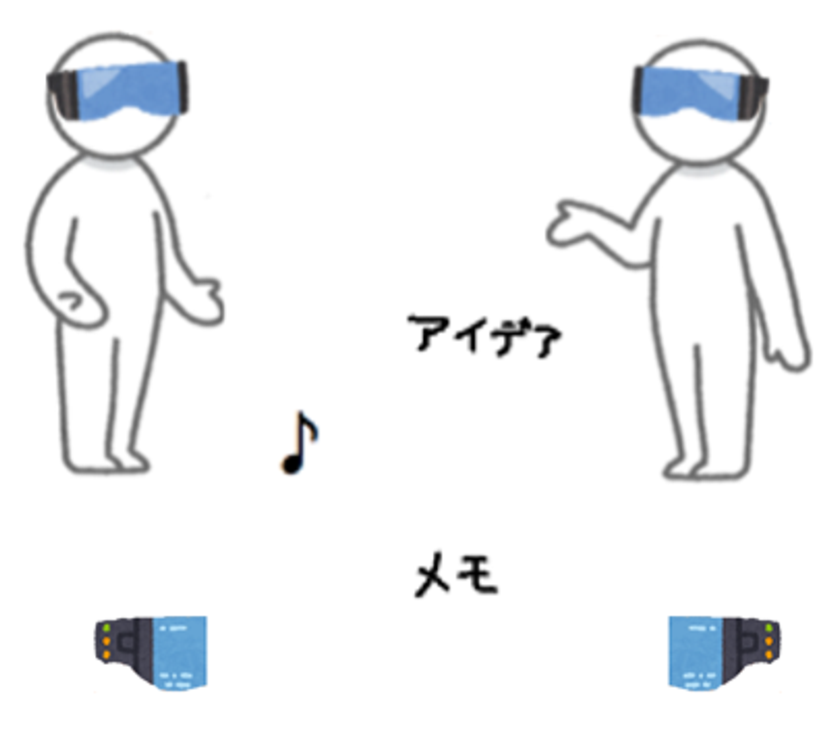
\includegraphics[clip,height=7.0cm,width=8.0cm]{./sharing_enkaku.eps}
    \caption{遠隔にいる相手にメモを共有}
    \label{fig:sharing_enkaku}
  \end{center}
\end{figure}


\newpage
\section{プロトタイプシステムの実装}
本章では、設計したシステムを基に行ったプロトタイプシステムの実装について述べる。

\subsection{プロトタイプシステムの構成}
設計されたシステムは、ユーザがシステムの各機能を利用するために使うアプリケーションと、HoloLens同士で相互接続するためのサーバ、ユーザが喋った内容をテキストに変換するクラウドサービスが存在する。図\ref{fig:prototypesystem}にプロトタイプシステムの全体図を示す。以下でそれぞれについて述べる。

\begin{figure}[H]
  \begin{center}
    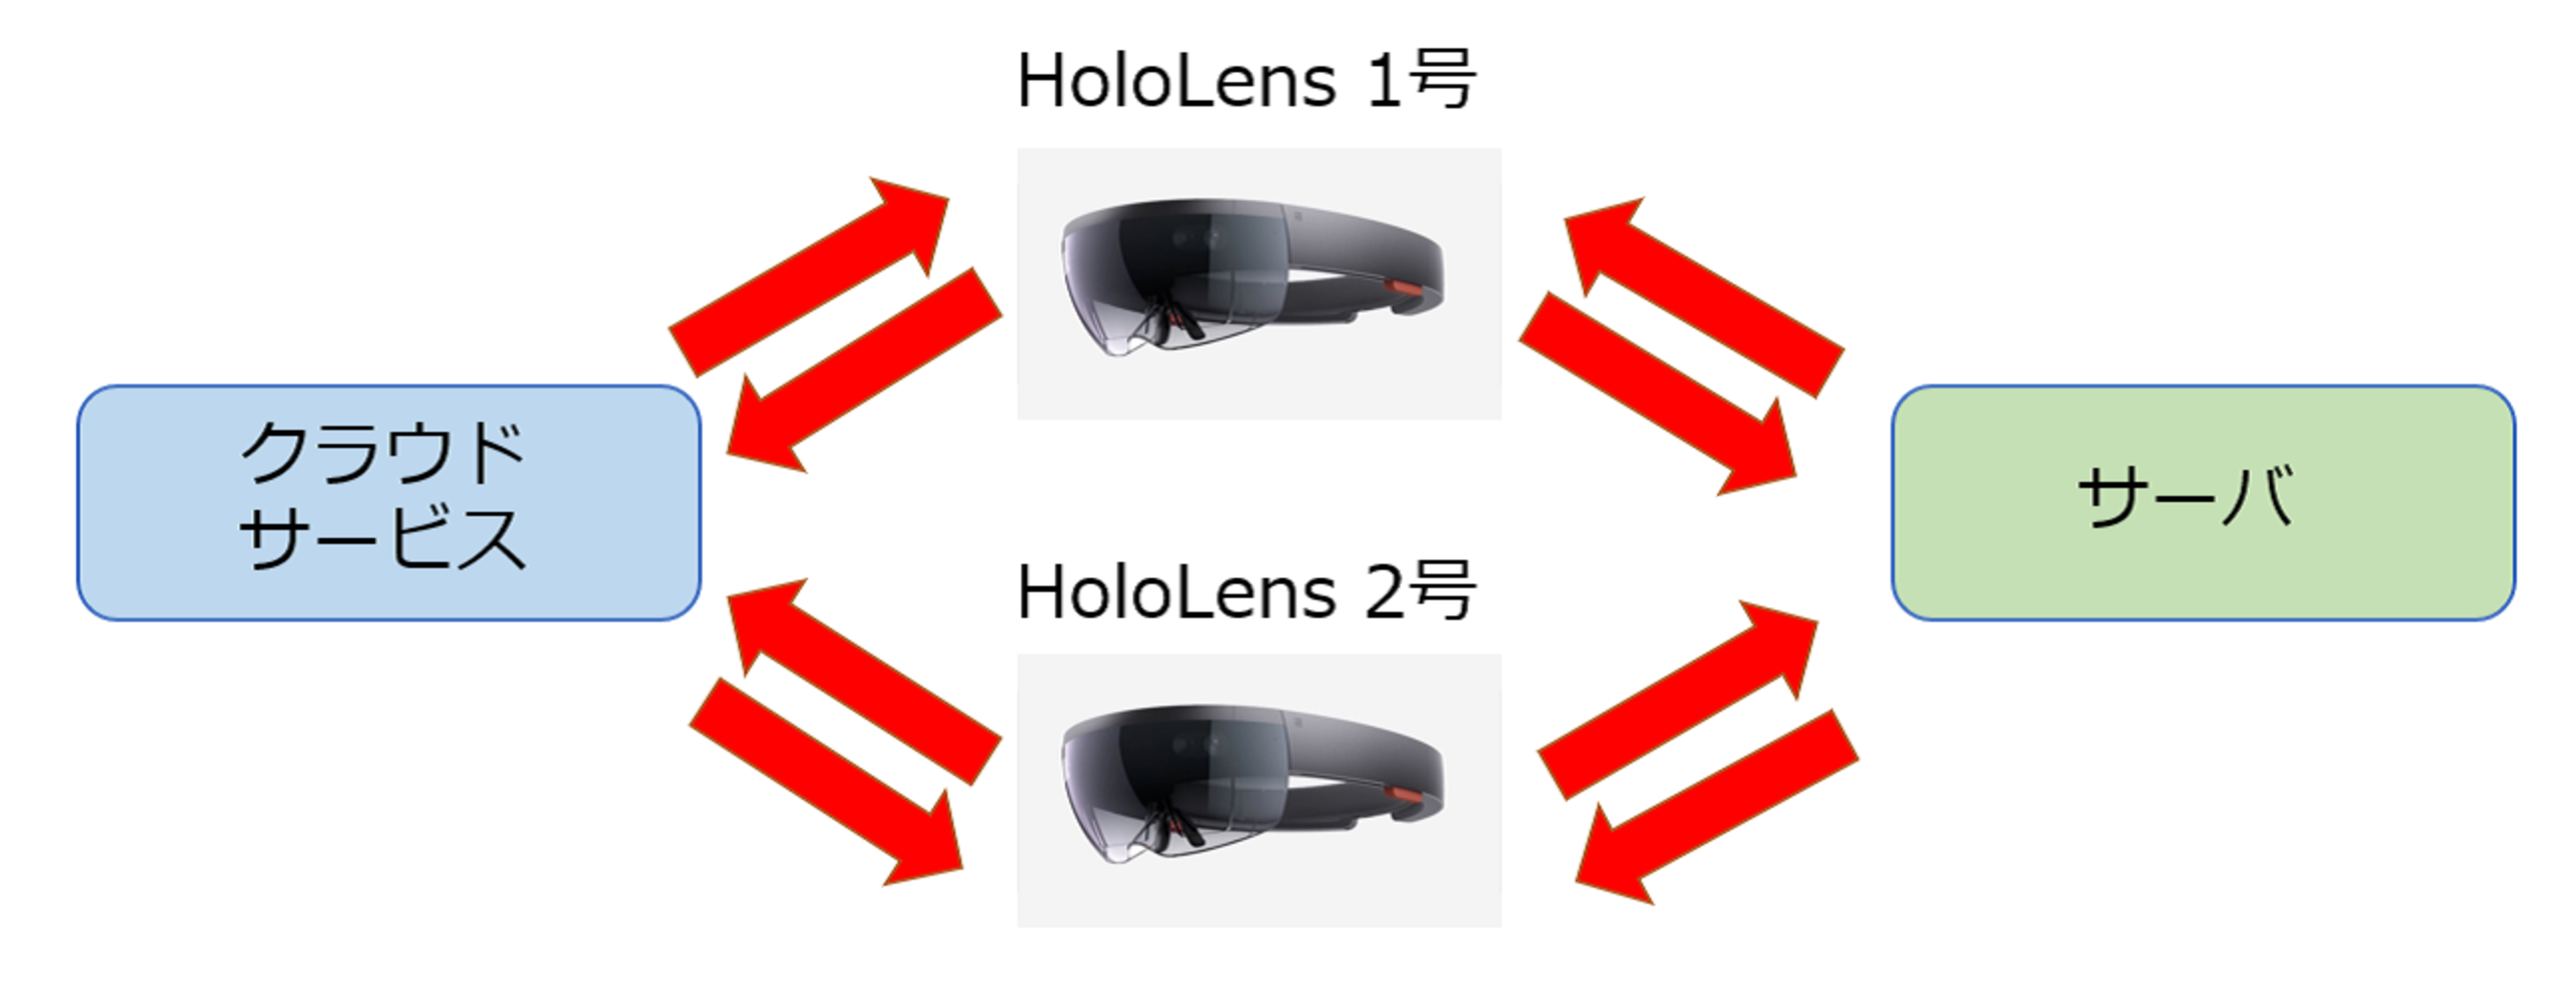
\includegraphics[clip,height=6.0cm,width=14.0cm]{./prototypesystem.eps}
    \caption{プロトタイプシステムの構成}
    \label{fig:prototypesystem}
  \end{center}
\end{figure}

\subsubsection{アプリケーション}
Windows 10やWindows 10 Mobile上で動作するUWP(Universal Windows Platform)アプリとして作成すると、HoloLens上でもそのアプリケーションが動作する。アプリケーションの開発には、マイクロソフト社が配布している統合開発環境であるVisual Studio 2017\cite{visualstudio}(Ver 15.0)と、ユニティ・テクノロジーズ社が配布している統合開発環境を内蔵した複数のプラットホームに対応するゲームエンジンであるUnity\cite{unity}(Ver 5.6.2f1)を使用した。また、Unity 用のHoloLens 向けのツールキットであるHoloToolkit-Unity\cite{holotoolkit}の導入を行った。開発言語には、Windows向けのアプリケーションの開発に主に使われるC\#を採用した。

\subsubsection{サーバ}
実世界の任意の空間上に残したメモを他のHoloLensを使用している人に共有するには、HoloToolkitのSharing\cite{sharing}という機能を利用し、Sharing用のサーバを介して空間の共有を行った。HoloLensの座標系は特殊であり、このまま共有をしても現実の空間の同じ位置で物体を共有することはできないという問題が発生する。この問題を解決するためにはアンカーの共有を行った(図\ref{fig:sharing})。アンカーとは船の錨の意味で空間内の絶対的な位置に居座ることができるオブジェクトのことである。これを設置することで位置合わせを行い、実世界の任意の空間上に残したメモの共有を行った。

\begin{figure}[H]
  \begin{center}
    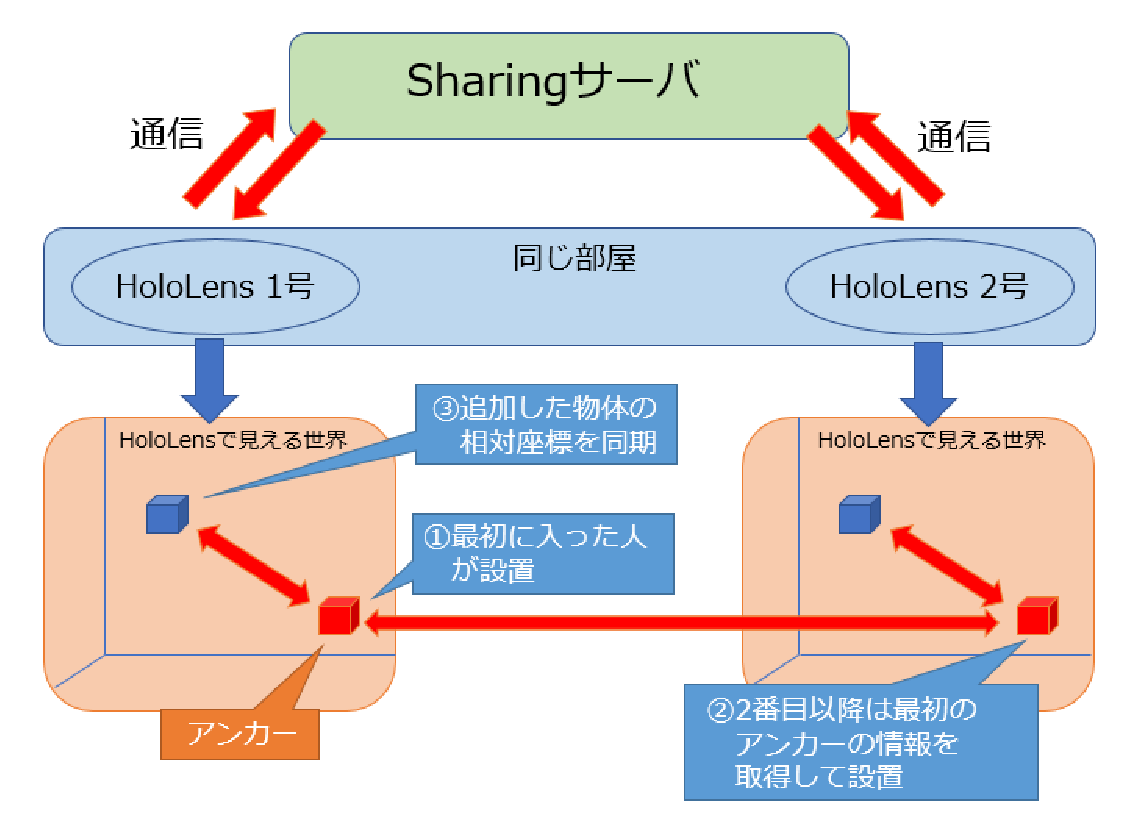
\includegraphics[clip,height=10.0cm,width=14.0cm]{./sharing.eps}
    \caption{アンカーを設置して座標の位置合わせを行い共有}
    \label{fig:sharing}
  \end{center}
\end{figure}

\subsubsection{クラウドサービス}
HoloLensの標準機能で音声入力はサポートされているが、現在利用できる言語が英語のみである\cite{emuniwa}。そこでGoogle Cloud Speech API\cite{google_speech}を利用することにより、日本語の音声をテキストに変換する(図\ref{fig:googlespeech})。Google Cloud Speech APIとはGoogleの持つ音声認識技術を使用し、音声をテキストに変換するサービスである。

\begin{figure}[H]
  \begin{center}
    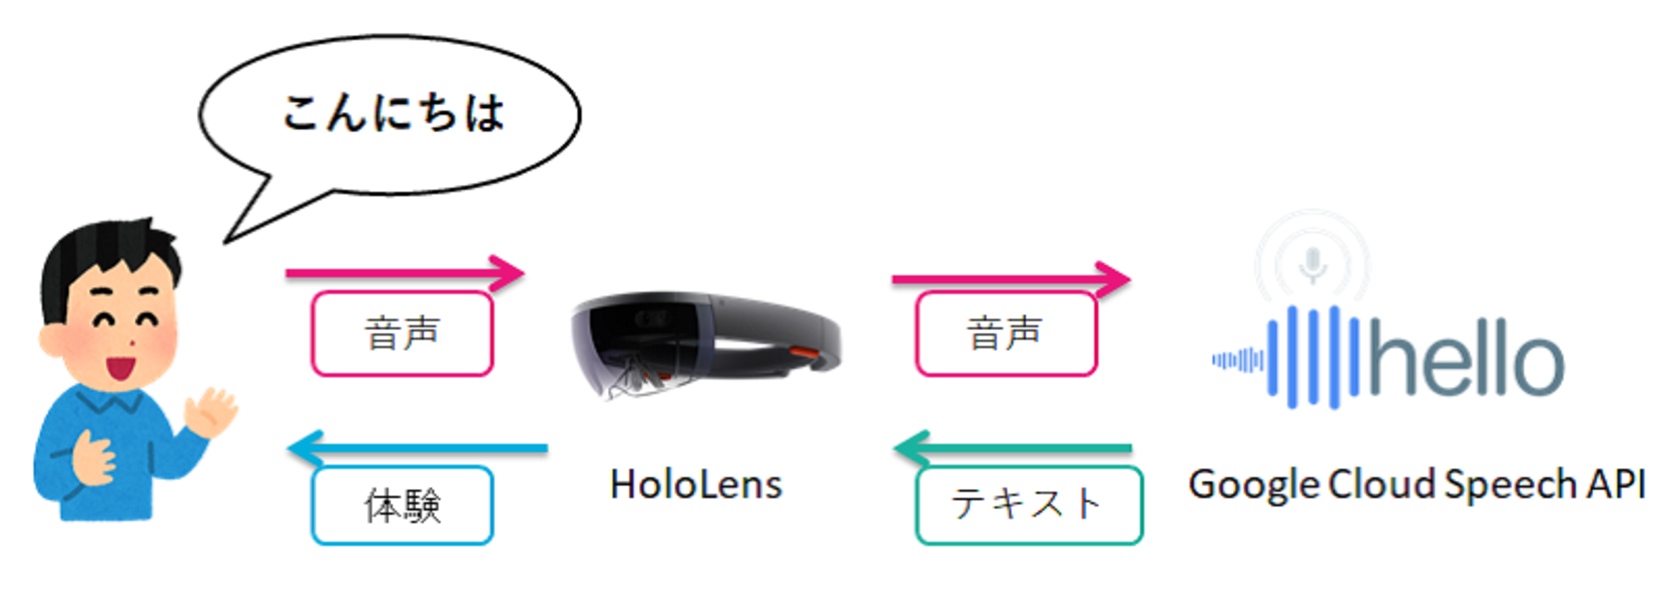
\includegraphics[clip,height=5.0cm,width=14.0cm]{./googlespeech.eps}
    \caption{日本語の音声をテキストに変換}
    \label{fig:googlespeech}
  \end{center}
\end{figure}

\subsection{プロトタイプの実装}

\subsubsection{全体構成}

\subsubsection{3D描画モード}

\subsubsection{付箋モード}

\subsubsection{Voice Lineモード}

\subsubsection{首振りモード}

\subsection{プロトタイプのデモンストレーション}

\newpage
\section{プロトタイプの評価実験}
本章では、実装したプロトタイプシステムの評価のために行った実験について述べる。

\subsection{実験の目的}
本実験は実装したプロトタイプシステムの機能が正常に動作するかどうかの確認を行うことと、システムに実装されているそれぞれの機能をユーザに使用してもらうことで提案システムの有用性について検証を行うことの2つを目的としている。

\subsection{実験の被験者}
本実験の被験者は男性9人と女性1人の合計10人で、情報系を専攻する大学生および大学院生である。平均年齢は23.7歳で、右利きの人が7人で左利きの人が3人である。HoloLensの使用経験について、全くないと回答したのが4人、少しあると回答したのが5人、よく使うと回答したのが1人である。

\subsection{実験環境}
本実験では実装したプロトタイプシステムのアプリケーションを2台のHoloLensにそれぞれインストールして用意をした。また、共有を行うためなるべく確実にネットワークに接続ができるように研究室内のゼミ室で行った(図\ref{fig:jikken_kankyo})。この実験では、被験者2人で1グループとして同時に行った。実験中に取り組んでもらうタスクに関する説明は、それぞれの被験者に渡せるように資料を作成して用意した。また、システムの機能の一部でキーボードを使用する箇所があるため、2つのBluetoothキーボードを用意した。

実験中の様子を図\ref{fig:jikkenchu}に示す。また、表\ref{table:jikken_kiki}に実験で使用した機器をまとめる。

\begin{figure}[H]
  \begin{center}
    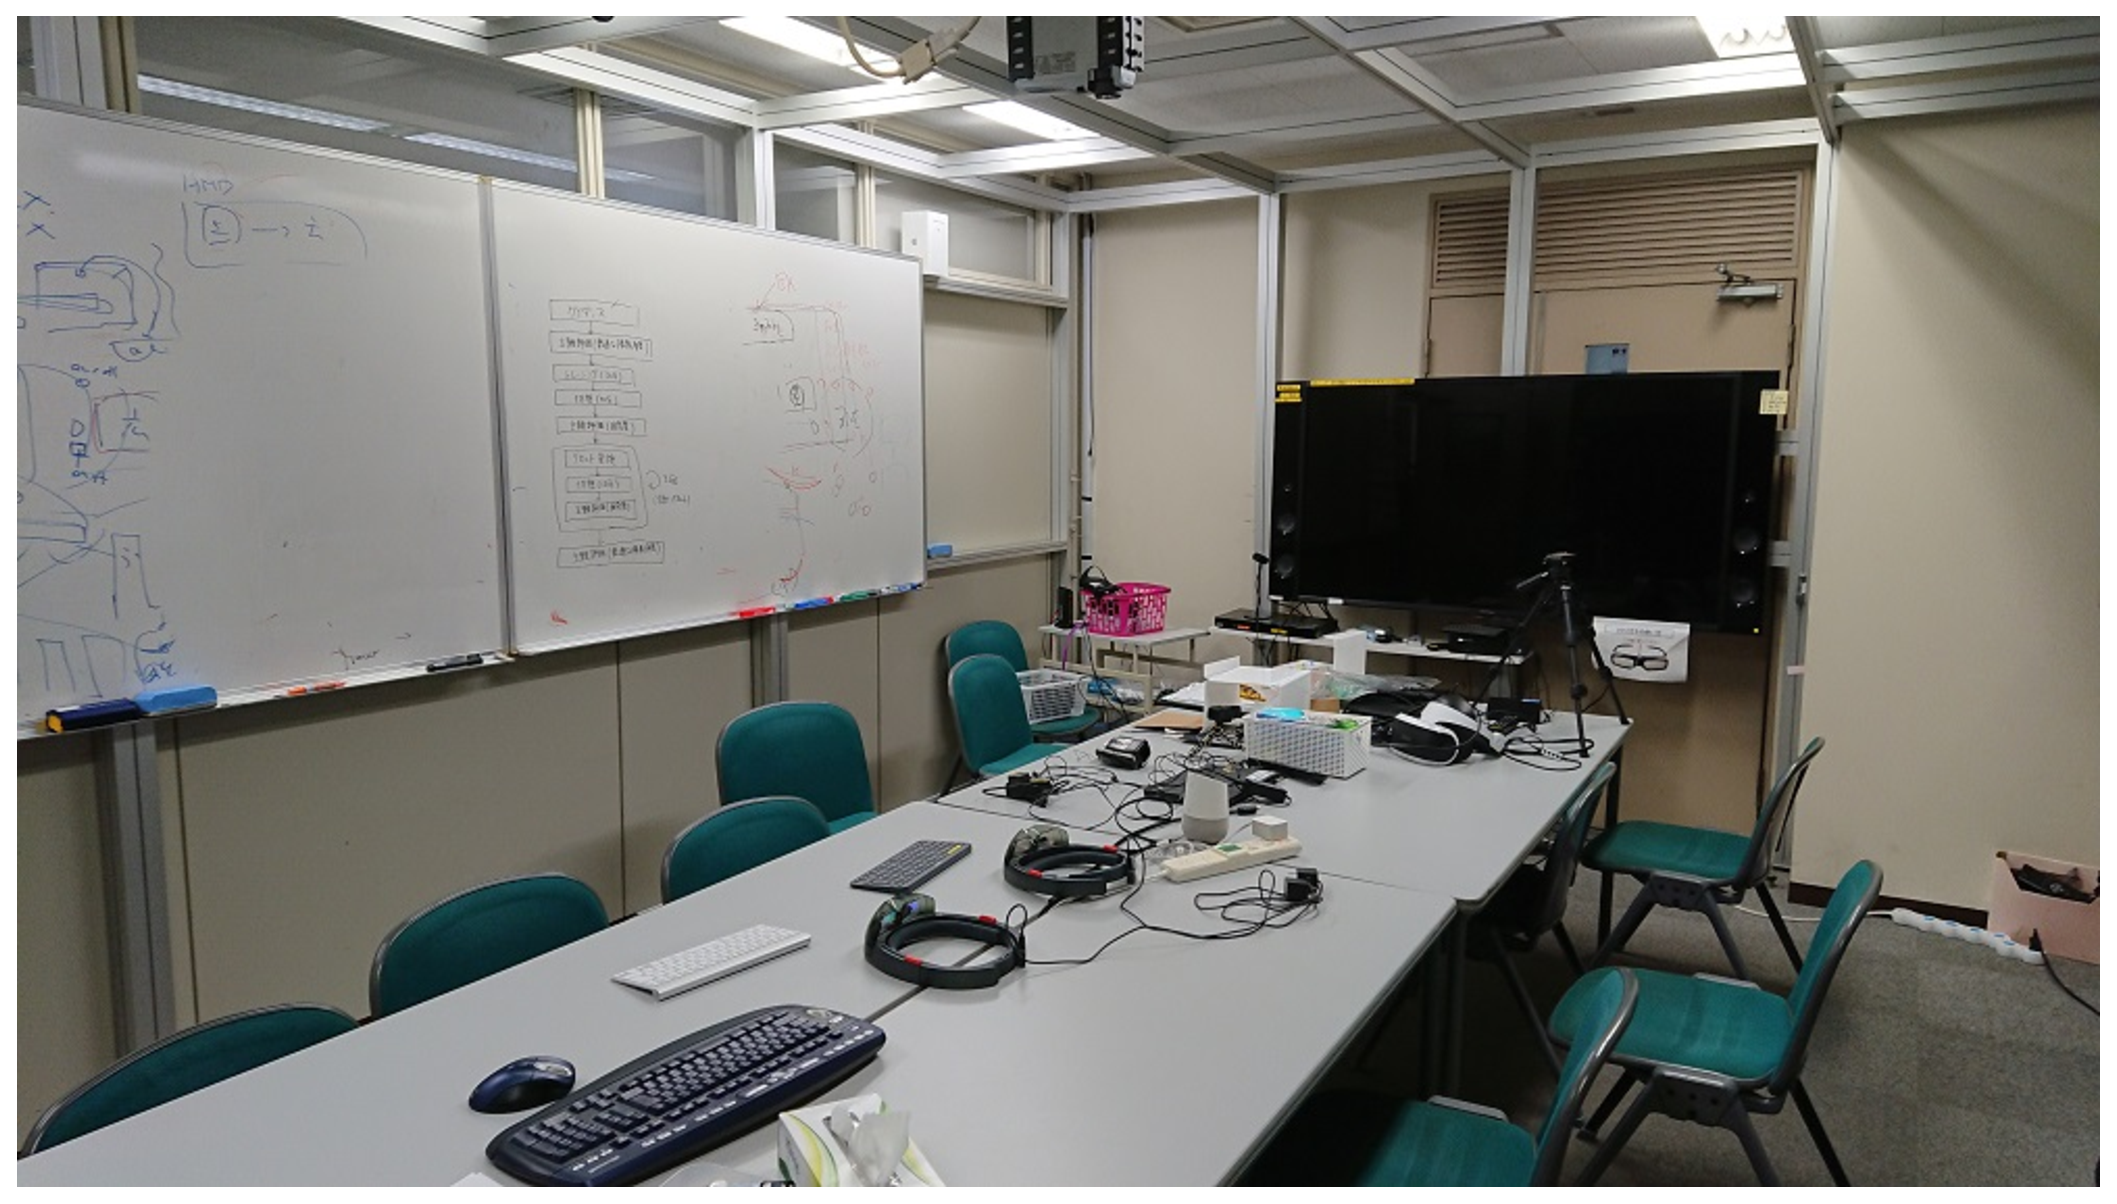
\includegraphics[clip,height=7.0cm,width=11.0cm]{./jikken_kankyo.eps}
    \caption{実験環境}
    \label{fig:jikken_kankyo}
  \end{center}
\end{figure}

\begin{figure}[H]
  \begin{center}
    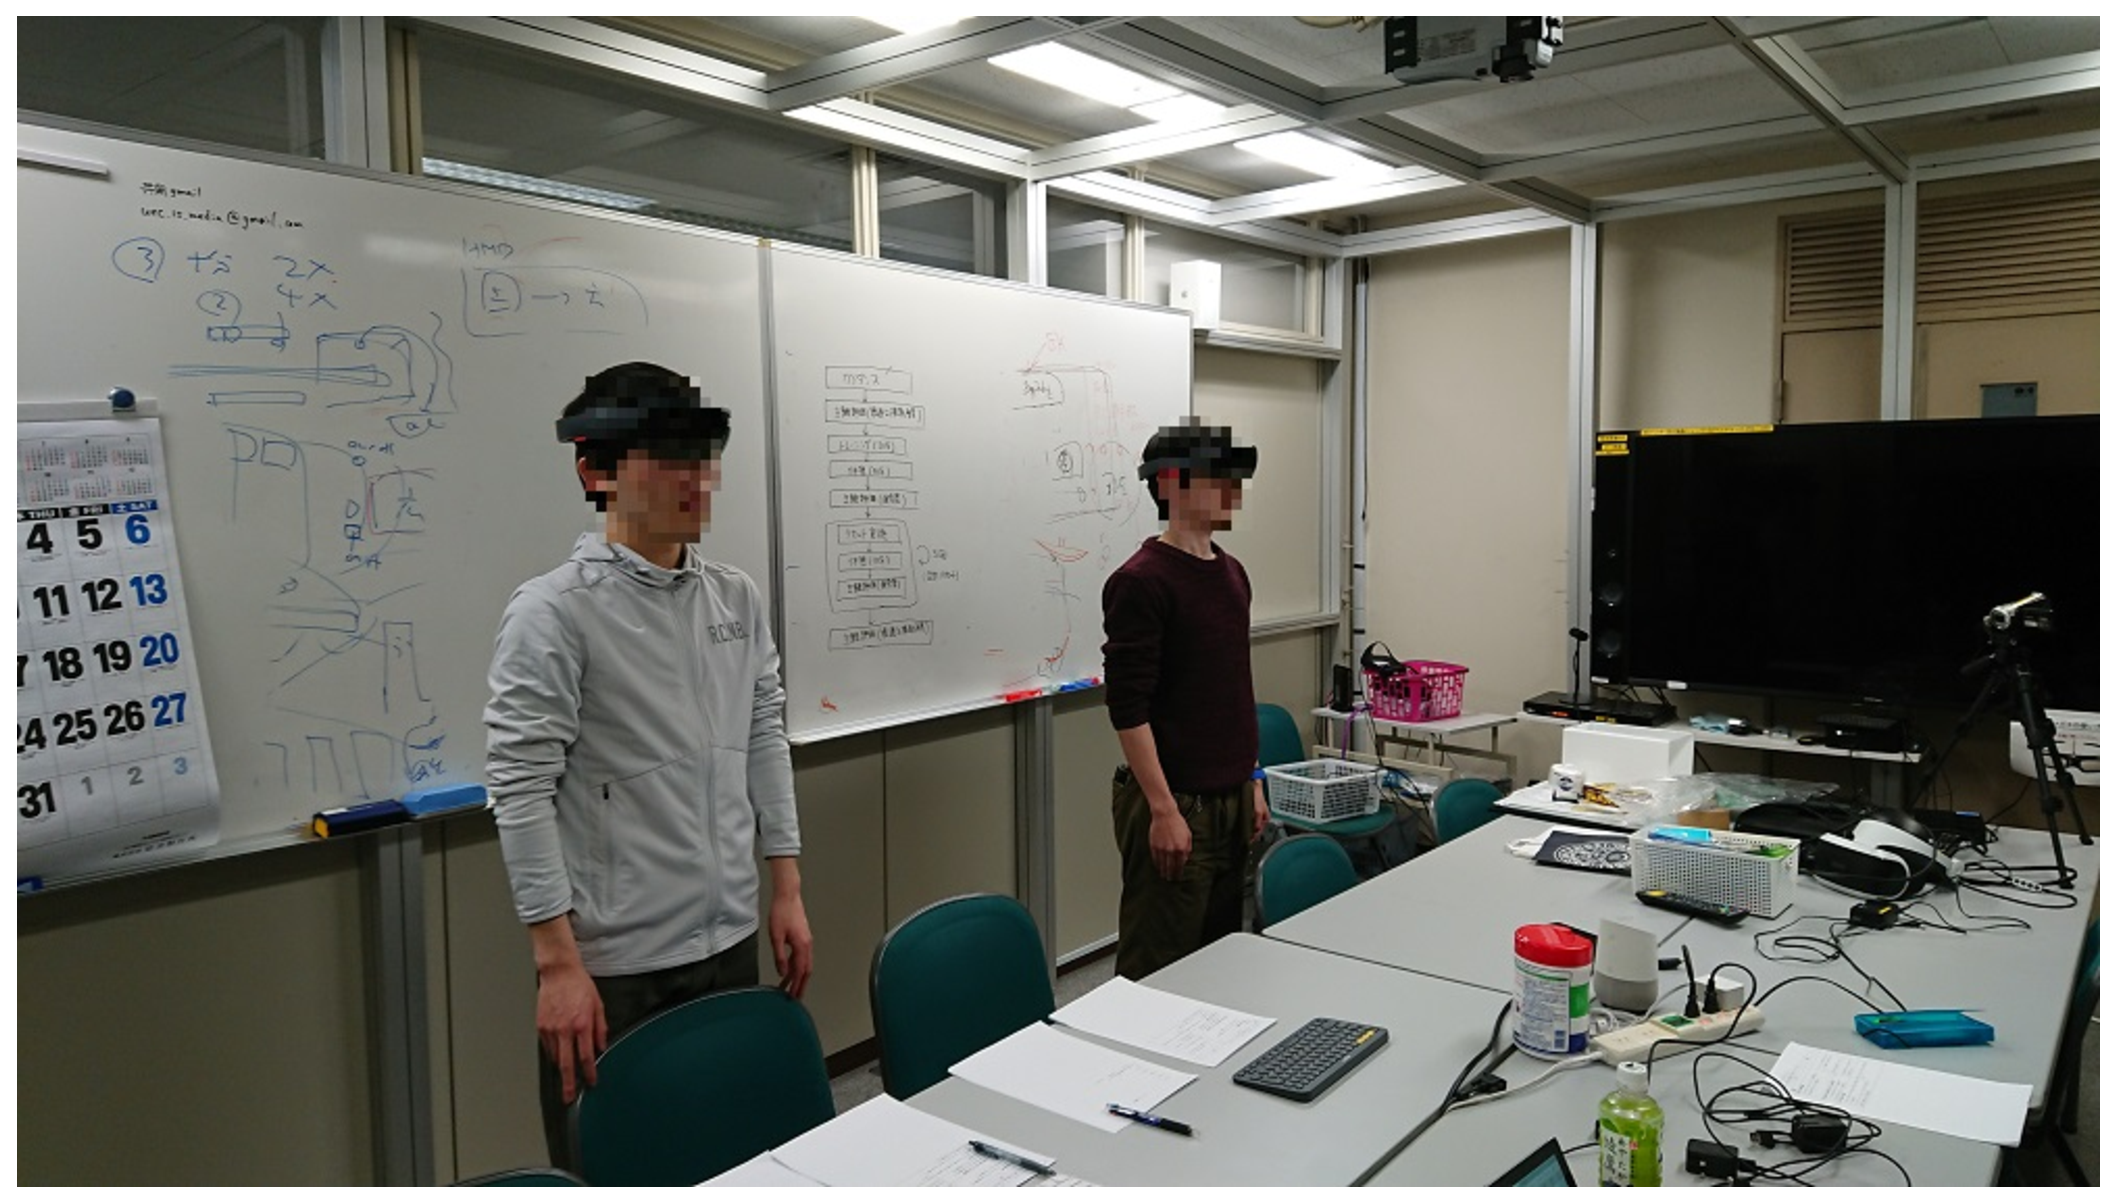
\includegraphics[clip,height=7.0cm,width=11.0cm]{./jikkenchu.eps}
    \caption{実験中の様子}
    \label{fig:jikkenchu}
  \end{center}
\end{figure}

\begin{table}[H]
\caption{実験で使用した機器}
\label{table:jikken_kiki}
\begin{center}
\begin{tabular}{|l|l|l|}
\hline
名称 & 型番 & メーカー \\
\hline\hline
ヘッドマウントディスプレイ & Microsoft HoloLens & Microsoft Inc. \\
\hline
ヘッドマウントディスプレイ & Microsoft HoloLens & Microsoft Inc. \\
\hline
Bluetoothキーボード & K380BK & 株式会社ロジクール \\
\hline
Bluetoothキーボード & MC184J/A & Apple Inc. \\
\hline
\end{tabular}
\end{center}
\end{table}

\subsection{実験方法}
本実験は以下に示す2つの作業から構成される。

\begin{itemize}
 \item シナリオ実験
 \item 課題解決実験
\end{itemize}

HoloLensを2台使用して共有を行うためそれぞれのタスクの前に準備を行った。それぞれで定められたタスクに取り組んでもらい、システムの動作状況やタスクの遂行状況などを確認して記録を行った。全てのタスクが終了した後に、プロトタイプシステムに関するアンケートに回答してもらった。各実験の詳細な手順についてを以下で述べる。

\subsubsection{準備}
それぞれのタスクを実際に行っていく前に、2台のHoloLensで共有を行うための準備を行った。まず1人目の被験者に所定の座席に座ってもらい、前方にある図のような図形を見てもらいながらHoloLensをかぶってアプリケーションを起動してもらった。1人目の起動が完了したら一度その座席から離れてもらい、2人目の被験者にも同様にその座席に座って前方にある図形を見てもらいながらアプリケーションを起動してもらった。2人目の起動が完了したら、それぞれのタスクに取り組んでもらうようにした。

\begin{figure}[H]
  \begin{center}
    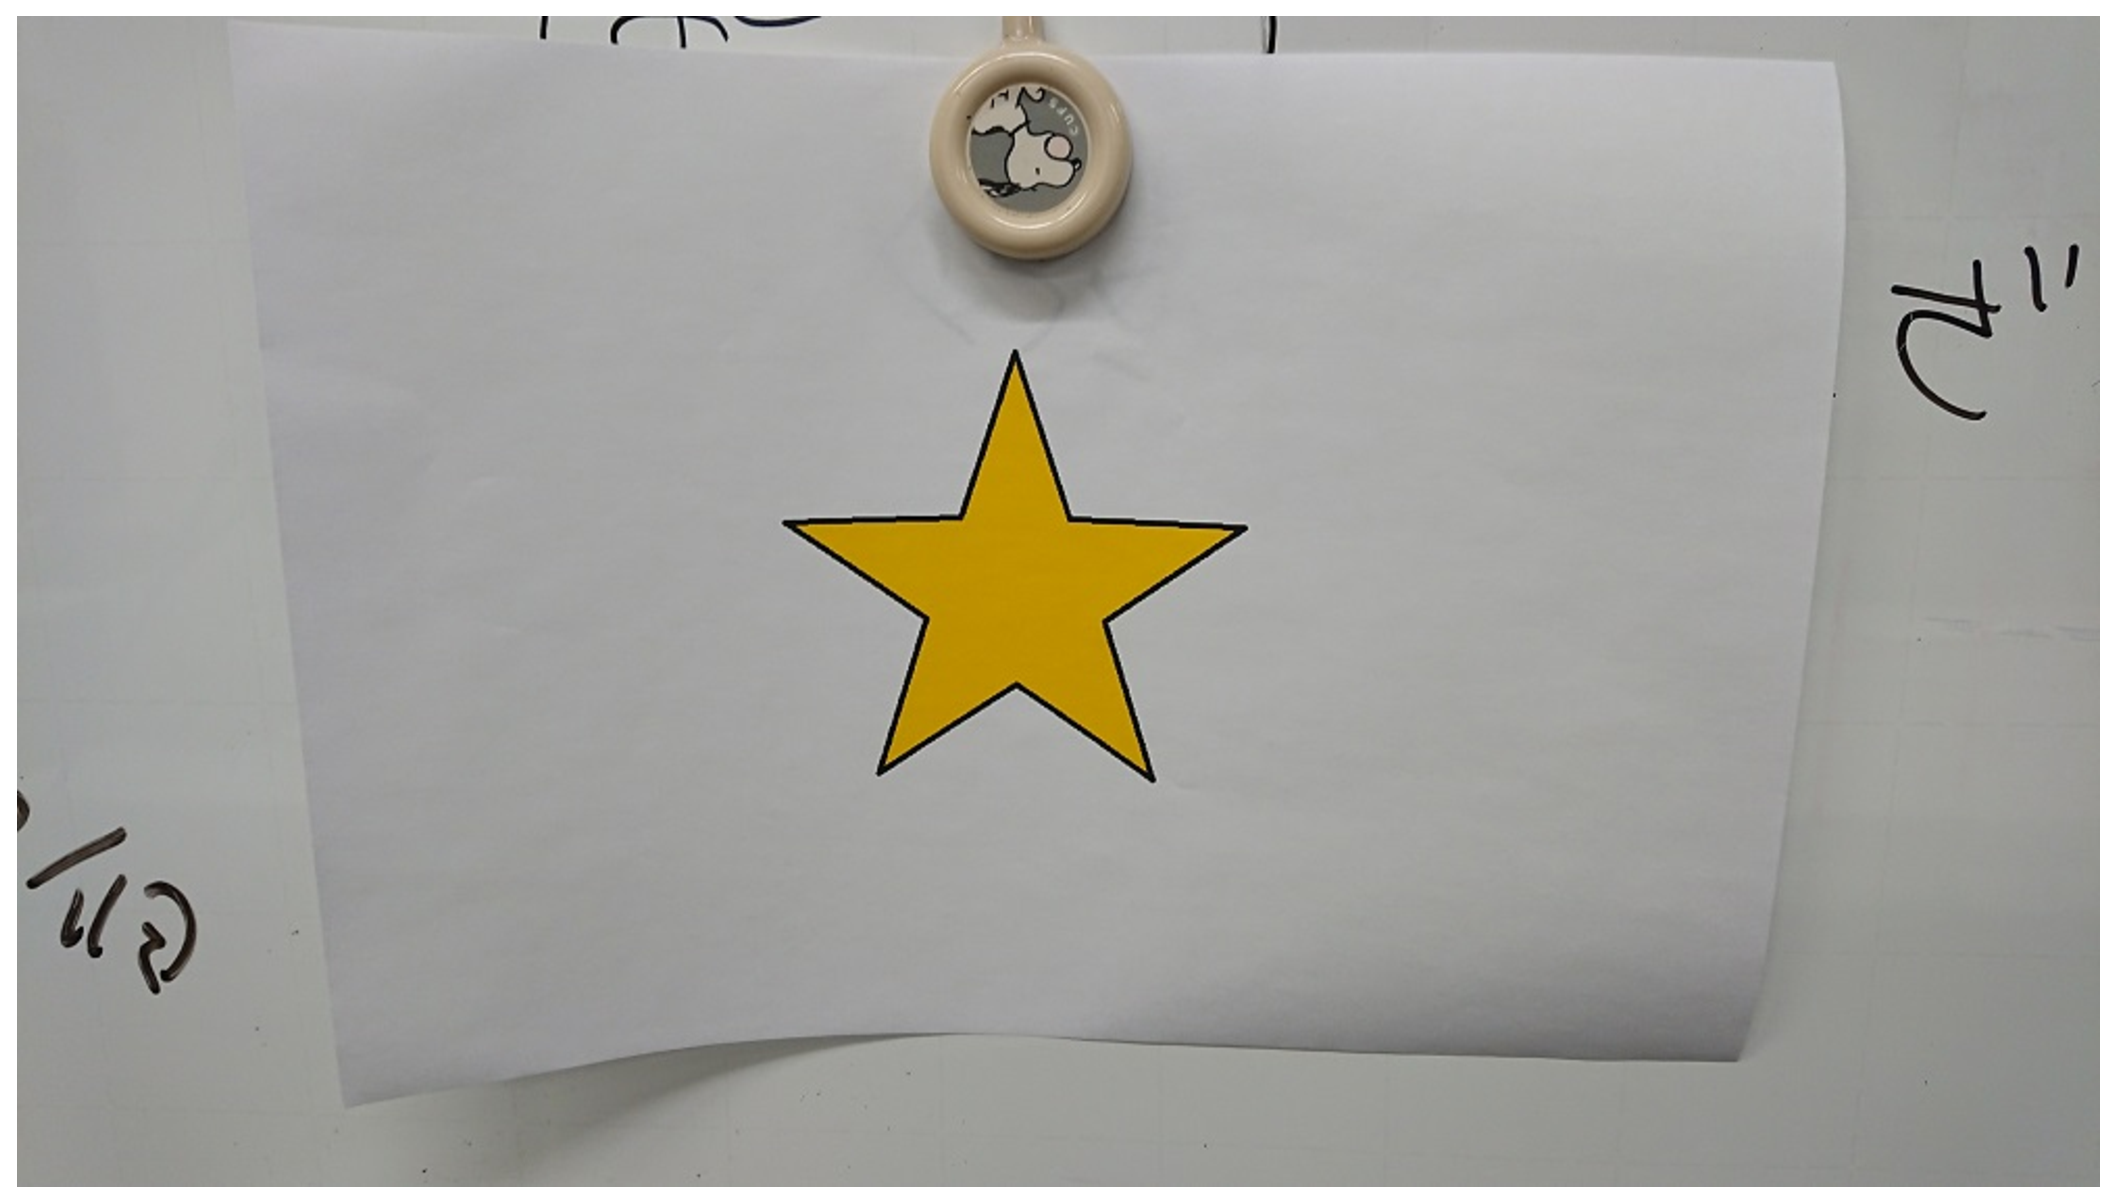
\includegraphics[clip,height=6.0cm,width=9.0cm]{./hoshi.eps}
    \caption{前方にある図形}
    \label{fig:hoshi}
  \end{center}
\end{figure}

\subsubsection{シナリオ実験}
シナリオ実験では、決められた手順に従ってそれぞれの被験者に操作をしてもらう。この手順は、プロトタイプシステムに実装されている全ての機能を使うように作られている。また、2人で同時に行って共有を行うため、1つの手順が終わったらそれぞれの被験者に完了したことを言うようにしてもらう。図\ref{fig:task1}~\ref{fig:task4}にシナリオ実験で取り組む手順が記された資料を、表\ref{table:task1}~\ref{table:task4}にシナリオの流れを示す。タスク1の内容は。この4つのタスクを一通り実施することで、プロトタイプシステムに実装されている機能の全てを体感することができる。

\begin{figure}[htbp]
 \begin{minipage}{0.5\hsize}
  \begin{center}
   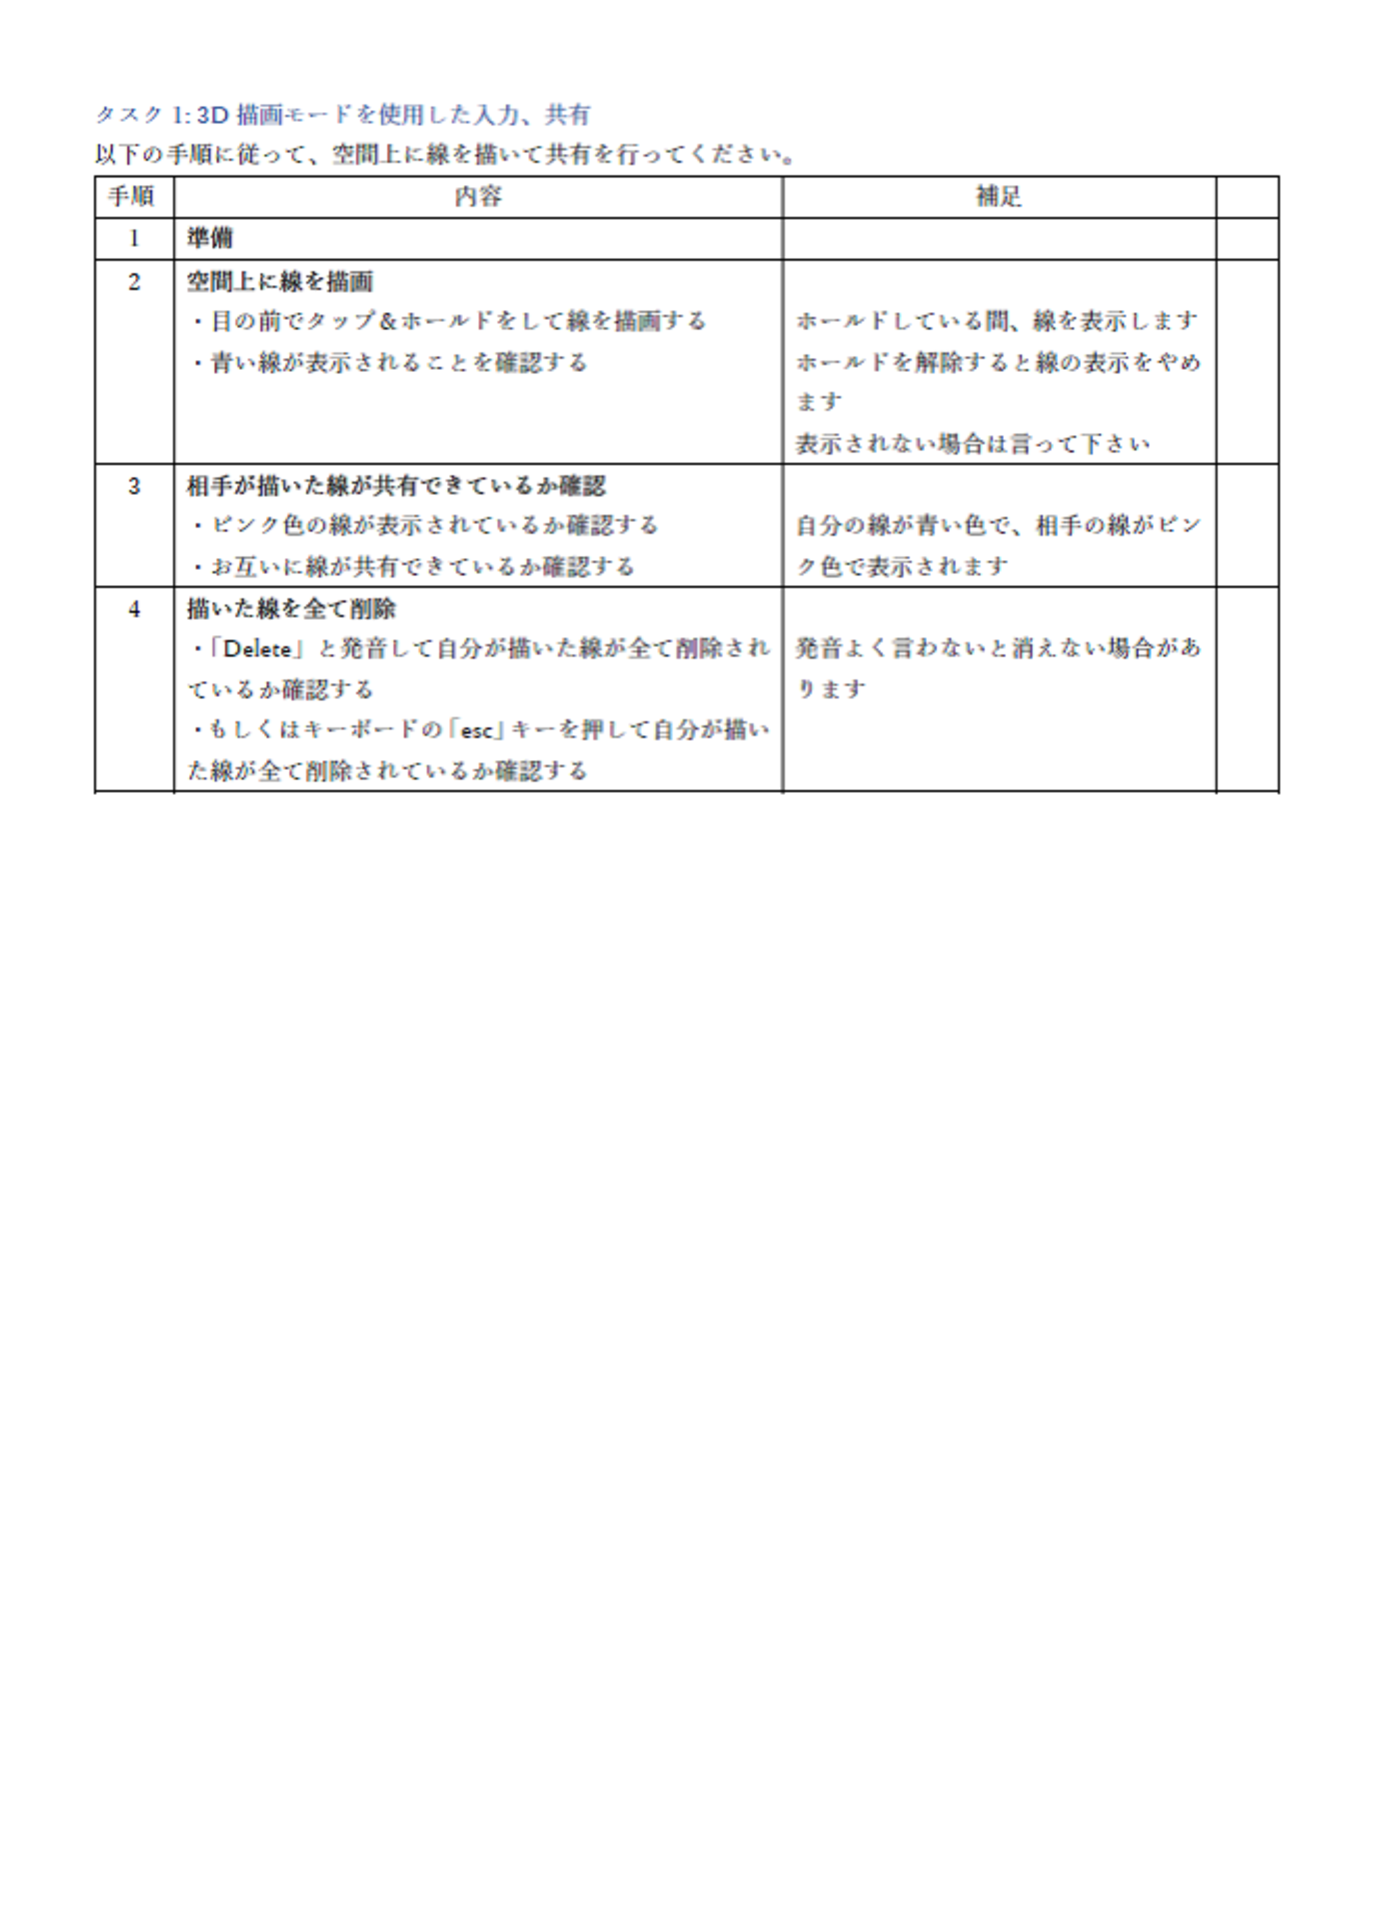
\includegraphics[width=70mm]{task1.eps}
  \end{center}
  \caption{シナリオ実験で掲示した資料:1枚目}
  \label{fig:task1}
 \end{minipage}
 \begin{minipage}{0.5\hsize}
  \begin{center}
   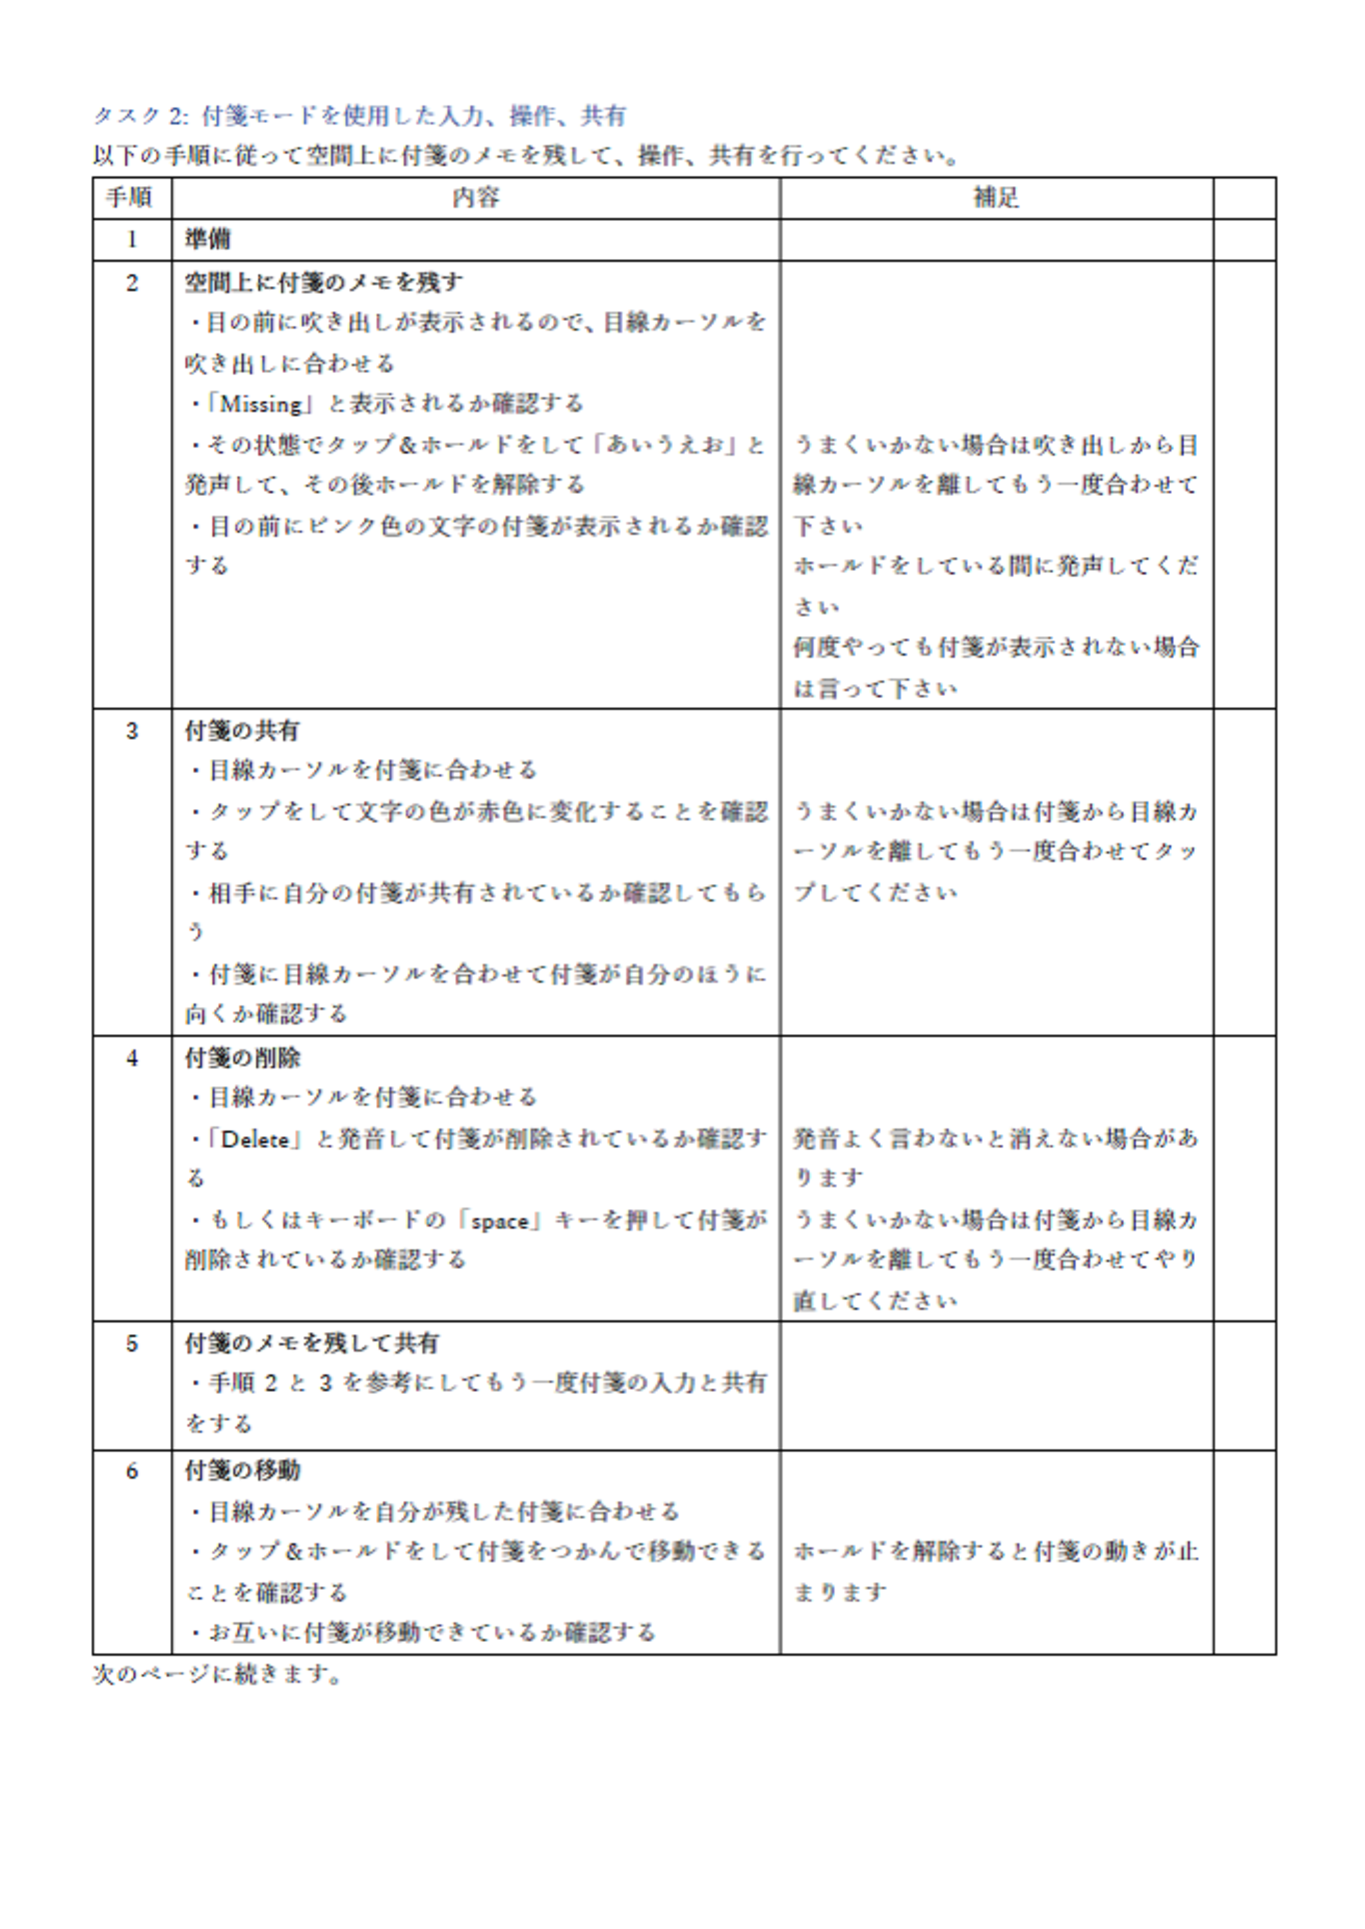
\includegraphics[width=70mm]{task2.eps}
  \end{center}
  \caption{シナリオ実験で掲示した資料:2枚目}
  \label{fig:task2}
 \end{minipage}
\end{figure}

\begin{figure}[htbp]
 \begin{minipage}{0.5\hsize}
  \begin{center}
   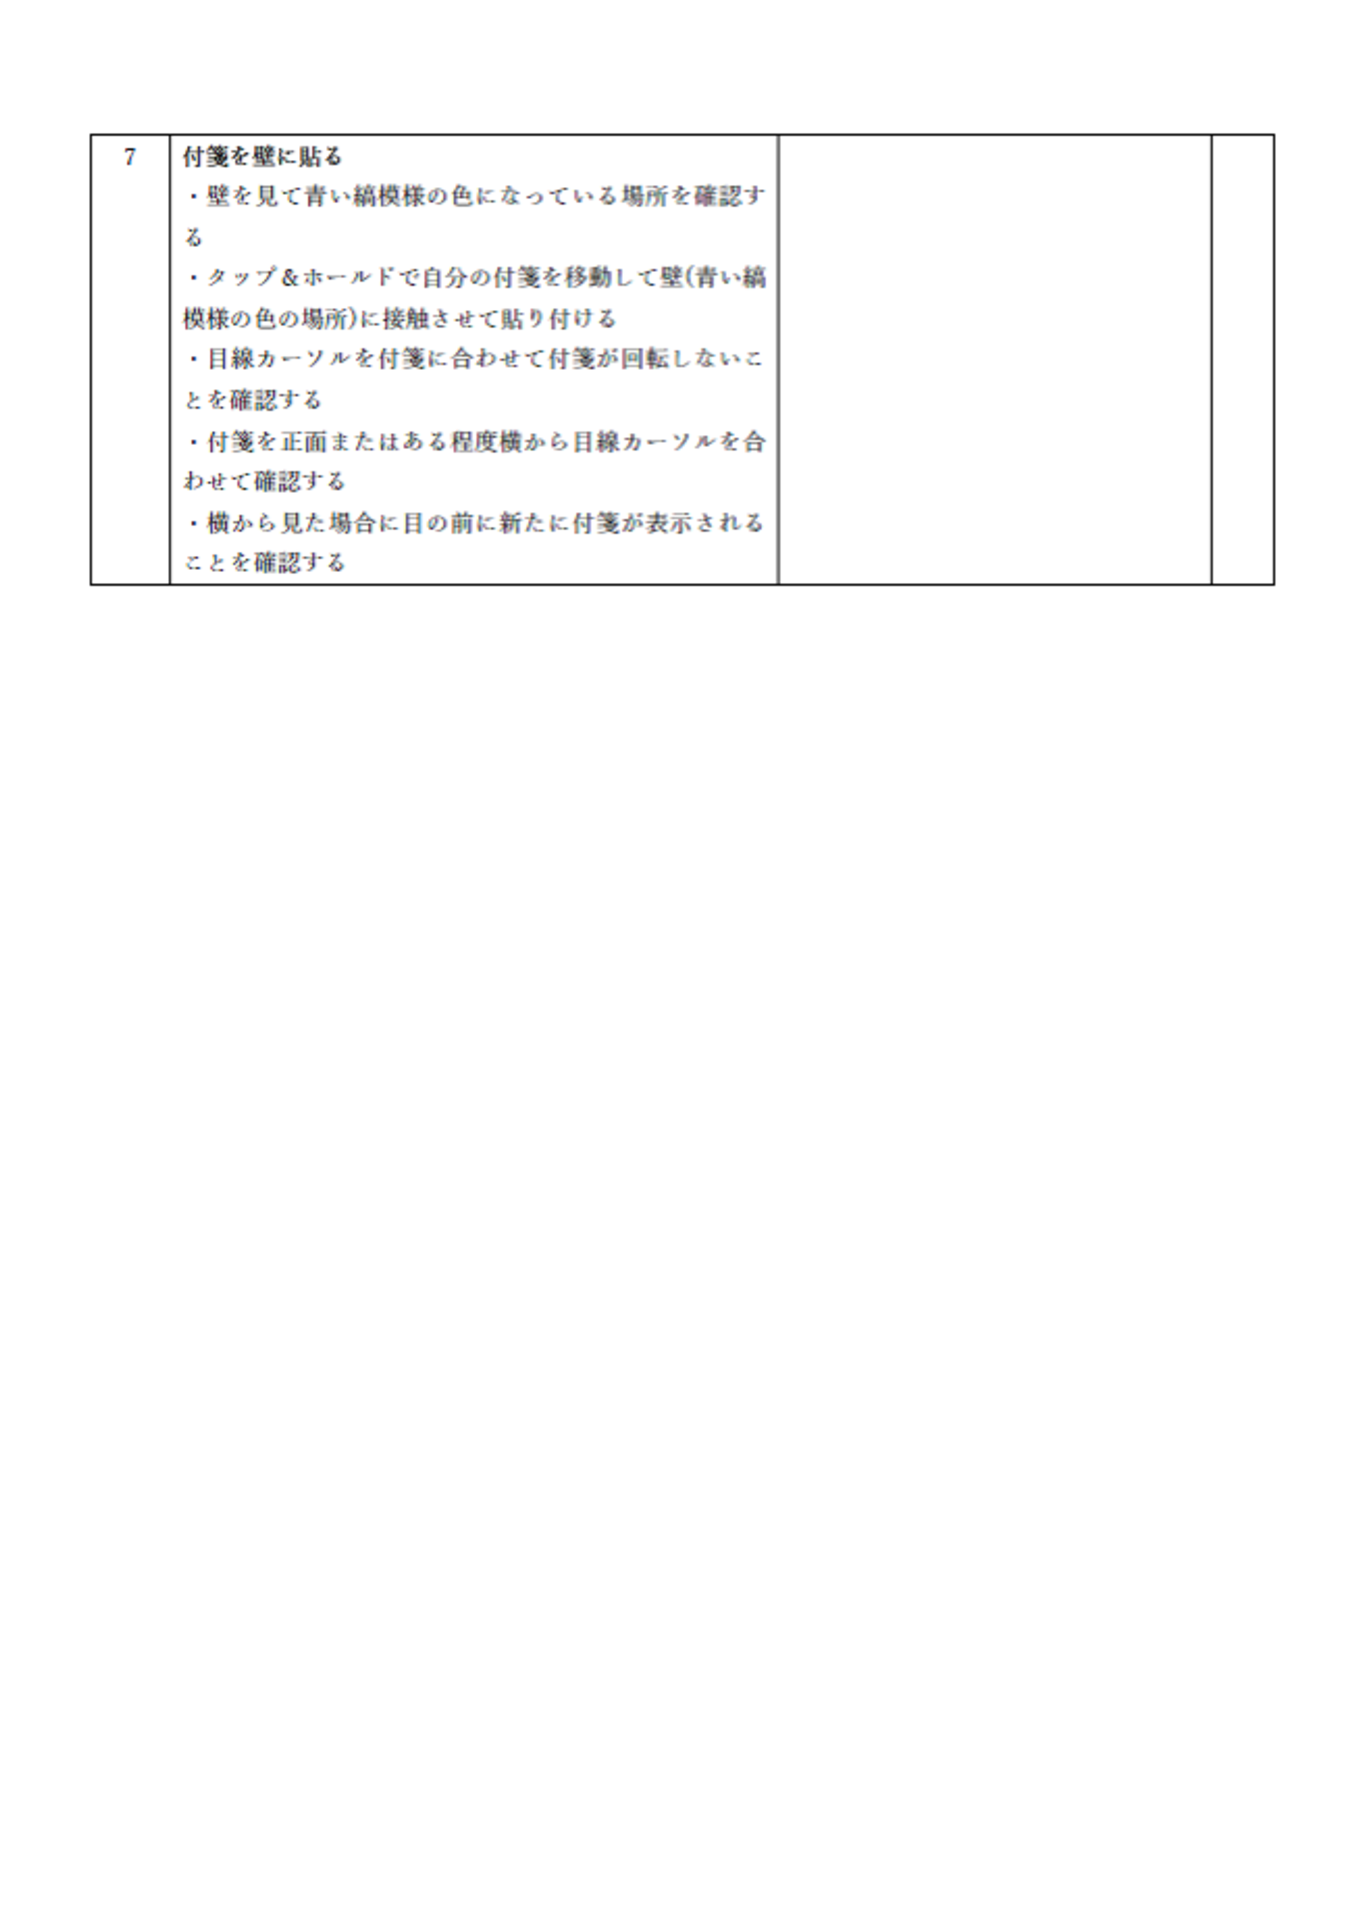
\includegraphics[width=70mm]{task2_2.eps}
  \end{center}
  \caption{シナリオ実験で掲示した資料:3枚目}
  \label{fig:task2_2}
 \end{minipage}
 \begin{minipage}{0.5\hsize}
  \begin{center}
   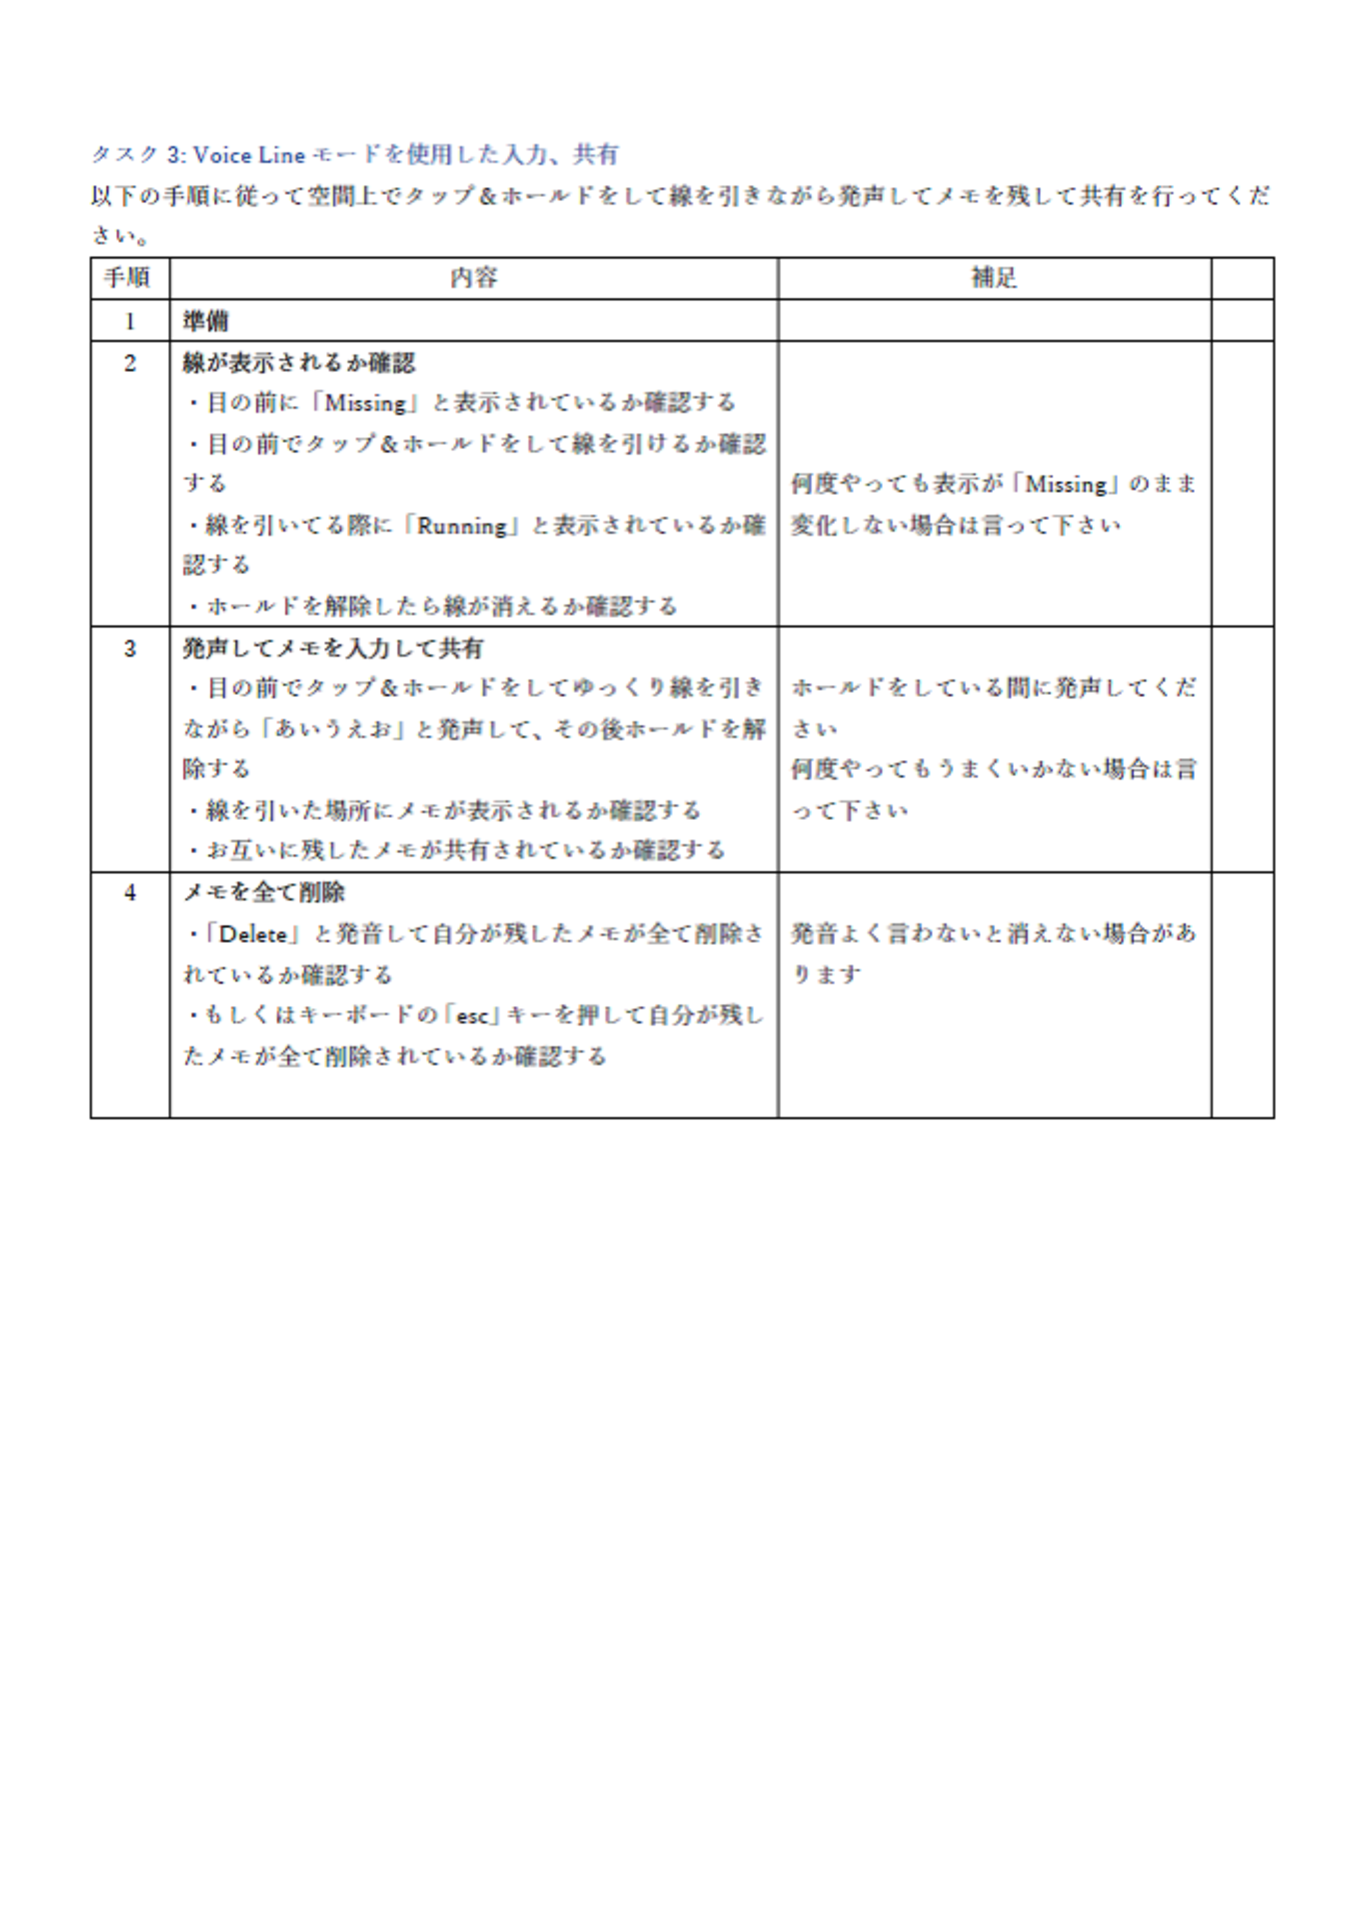
\includegraphics[width=70mm]{task3.eps}
  \end{center}
  \caption{シナリオ実験で掲示した資料:4枚目}
  \label{fig:task3}
 \end{minipage}
\end{figure}

\begin{figure}[H]
  \begin{center}
    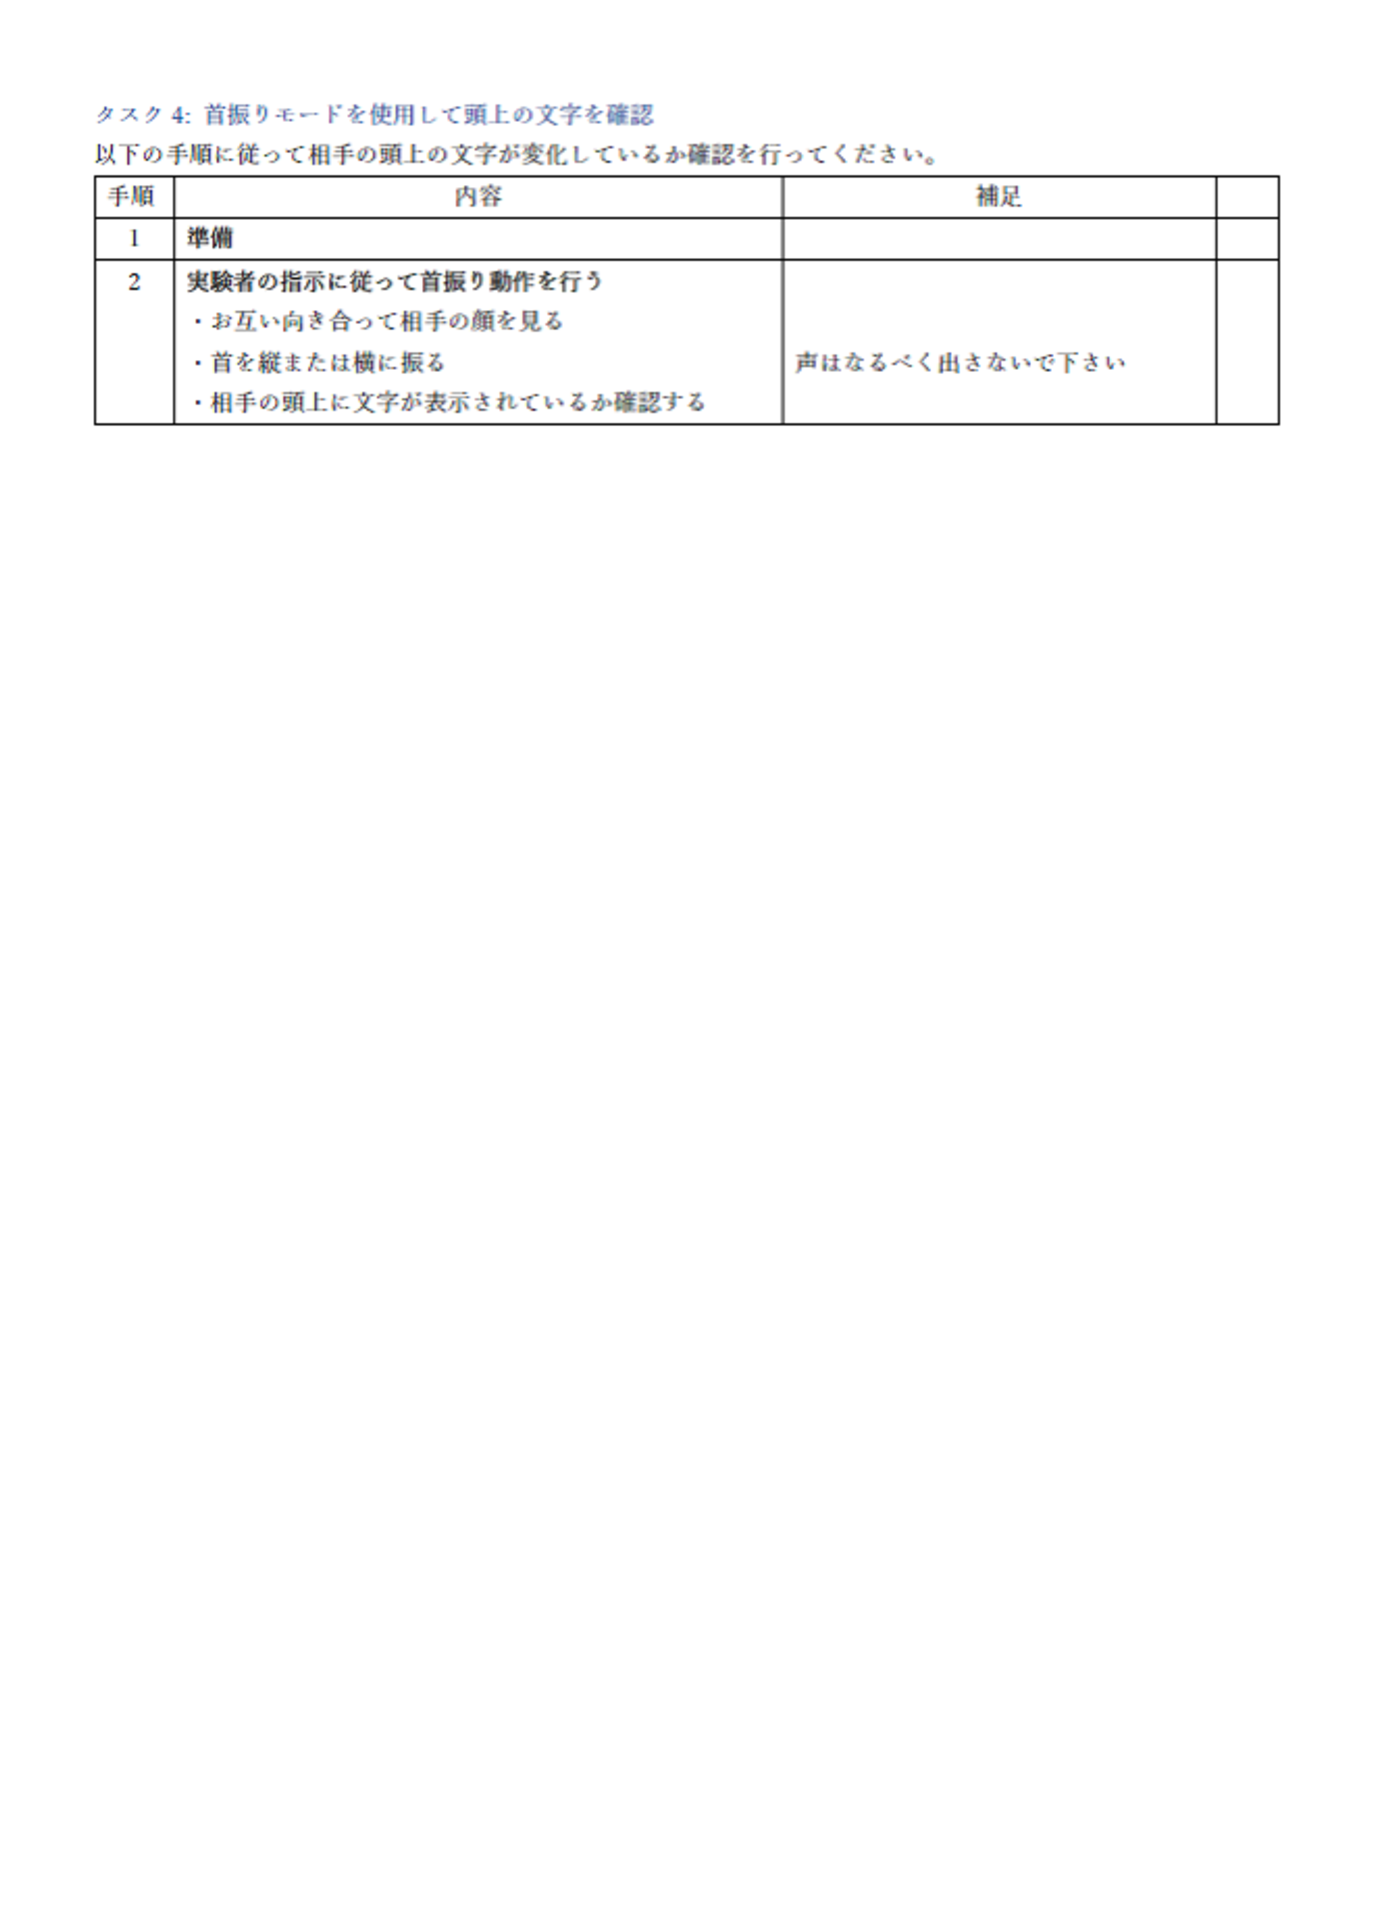
\includegraphics[clip,height=9.0cm,width=7.0cm]{./task4.eps}
    \caption{課題解決実験で掲示した資料}
    \label{fig:task4}
  \end{center}
\end{figure}

\begin{table}[H]
\caption{タスク1:3D描画モードを使用した入力、共有}
\label{table:task1}
\begin{center}
\begin{tabular}{|c|c|}
\hline
手順 & 内容  \\
\hline\hline
1 & 準備  \\
\hline
2 & 空間上に線を描画  \\
\hline
3 & 相手が描いた線が共有できているか確認 \\
\hline
4 & 描いた線を全て削除  \\
\hline
\end{tabular}
\end{center}
\end{table}

\begin{table}[H]
\caption{タスク2:付箋モードを使用した入力、操作、共有}
\label{table:task2}
\begin{center}
\begin{tabular}{|c|c|}
\hline
手順 & 内容  \\
\hline\hline
1 & 準備  \\
\hline
2 & 空間上に付箋のメモを残す  \\
\hline
3 & 付箋の共有 \\
\hline
4 & 付箋の削除  \\
\hline
5 & 付箋のメモを残して共有  \\
\hline
6 & 付箋の移動 \\
\hline
7 & 付箋を壁に貼る \\
\hline
\end{tabular}
\end{center}
\end{table}

\begin{table}[H]
\caption{タスク3:Voice Lineモードを使用した入力、共有}
\label{table:task3}
\begin{center}
\begin{tabular}{|c|c|}
\hline
手順 & 内容  \\
\hline\hline
1 & 準備  \\
\hline
2 & 線が表示されるか確認  \\
\hline
3 & 発声してメモを入力して共有 \\
\hline
4 & メモを全て削除  \\
\hline
\end{tabular}
\end{center}
\end{table}

\begin{table}[H]
\caption{タスク4:首振りモードを使用して頭上の文字を確認}
\label{table:task4}
\begin{center}
\begin{tabular}{|c|c|}
\hline
手順 & 内容  \\
\hline\hline
1 & 準備  \\
\hline
2 & 実験者の指示に従って首振り動作を行う  \\
\hline
\end{tabular}
\end{center}
\end{table}

\subsubsection{課題解決実験}
課題解決実験では、シナリオ実験のような詳細な操作手順は用意しない。代わりに簡単な課題を被験者に出して、プロトタイプシステムを用いてその課題を解決するように指示した。被験者は、先に実施するシナリオ実験においてプロトタイプシステムの操作を一通り終えているので、被験者が自ら考えてプロトタイプシステムを操作して課題を解決することになる。図\ref{fig:task5}に、課題解決実験で掲示した資料を示す。

\begin{figure}[H]
  \begin{center}
    \includegraphics[clip,height=9.0cm,width=7.0cm]{./task5.eps}
    \caption{課題解決実験で掲示した資料}
    \label{fig:task5}
  \end{center}
\end{figure}

\subsection{実験結果と考察}
まず、シナリオ実験に関するタスク1~4の達成状況について、表\ref{table:jikken_kekka}に示す。表中の各セルには、被験者が各手順をどの程度達成できたかが3段階で示されている。〇の場合、被験者はその手順について特に支障なく完了したことを示す。△の場合、手順の進め方が分からない等の理由で実験者へ質問等があり、被験者は実験者からの助言を元に手順を完了したことを示す。×の場合、その手順を完了させることができなかったことを示す。

表\ref{table:jikken_kekka}よりタスク1~4のほとんどの手順で成功率が100\%となった。一方で、タスク1で手順2において支障なくタスクの完了ができない被験者が1名確認された。手順2は、目の前でタップ&ホールドをして線を描画して、青い線が表示されることを確認するというものである。実験中に被験者Dから線の描画される位置がおかしいという申告があったため確認を行った。その結果、線の描画の位置はややズレはあったが表示はされていた。原因としては正しくタップができていない、またはHoloLensを正しく装着できていない等が考えられる。また、3D描画モードの線を描くときに位置が若干ズレが生じるのは仕様であるため、線の描画される位置を少し補正する等の処理が必要だったと考えられる。線の描画の表示自体は正しく行われていたので、そのまま被験者Dには手順を進めてもらった。

タスク2では手順7において支障なくタスクの完了ができない被験者が1名確認された。手順7は、空間上に残した付箋を壁に貼るというものである。実験中に被験者Hから付箋を壁に貼り付けようとしたら付箋が消えてしまったという申告があったため確認を行った。その結果、付箋が確かに被験者Hから見えないことがわかった。しかし、同時に実験を行っていた被験者Gからは消えたその付箋が見えるという報告があった。付箋モードでは機能を選択したときに最初に実世界の空間上を認識して壁を綺麗な平面として生成する処理を行っている。被験者Hのほうでは空間上の一部分を正しく認識しなかったため、壁を綺麗な平面として生成できなかった可能性がある。そこに付箋を移動して持っていって実世界の壁の向こう側に行ってしまい、生成した近くの平面に接触したため、平面の裏側に付箋が貼り付いてしまったからだと考えられる。被験者Hにはもう一度付箋を残してもらって壁に貼り付けてもらった結果、うまく貼り付いたとの報告があったのでそのまま手順を進めてもらった。

タスク4では手順2において支障なくタスクの完了ができない被験者が1名確認された。手順2は、実験者の指示に従って首振り動作を行ってもらいお互いの頭上の文字が変化しているか確認するというものである。実験中に被験者Hから相手の頭上の文字の表示がおかしいという申告があったため確認を行った。その結果、相手が首を縦に振ったのにも限らずNoと表示されてしまうことがわかった。何度も行ってもらっても変わらなかったため、被験者GとHのHoloLensを再起動し、もう一度手順1からやり直してもらった。その結果、少し改善されたとの報告があったのでそのまま手順を進めてもらった。原因として相手の被験者Gが縦に首振りをする際に、わずかに横に振ってしまい頭上にNoと表示されてしまったのではないかと考えられる。また、実験中被験者Hは手順1の準備で他の被験者と比較して明らかに時間がかかっていたため、ネットワークの状態があまり良くなかったのではないかと考えられる。

以上の結果から、本シナリオ実験によってほぼ全ての手順を支障なく完了することができたことがわかった。

\begin{table}[H]
  \caption{被験者A~Jのシナリオ実験の結果}
  \label{table:jikken_kekka}
  \begin{center}
  \begin{tabular}{|c||c|c|c|c|c|c|c|c|c|c|c||c|} \hline
    タスク & 手順 & A & B & C & D & E & F & G & H & I & J & 成功率 \\ \hline \hline
             & 1 & 〇 & 〇 & 〇 & 〇 & 〇 & 〇 & 〇 & 〇 & 〇 & 〇 & 100\% \\ \cline{2-13}
    タスク1 & 2 & 〇 & 〇 & 〇 & △ & 〇 & 〇 & 〇 & 〇 & 〇 & 〇 &  90\% \\ \cline{2-13}
             & 3 & 〇 & 〇 & 〇 & 〇 & 〇 & 〇 & 〇 & 〇 & 〇 & 〇 & 100\% \\ \cline{2-13}
             & 4 & 〇 & 〇 & 〇 & 〇 & 〇 & 〇 & 〇 & 〇 & 〇 & 〇 & 100\% \\ \cline{2-13} \hline \hline
             & 1 & 〇 & 〇 & 〇 & 〇 & 〇 & 〇 & 〇 & 〇 & 〇 & 〇 & 100\% \\ \cline{2-13}
             & 2 & 〇 & 〇 & 〇 & 〇 & 〇 & 〇 & 〇 & 〇 & 〇 & 〇 & 100\% \\ \cline{2-13}
             & 3 & 〇 & 〇 & 〇 & 〇 & 〇 & 〇 & 〇 & 〇 & 〇 & 〇 & 100\% \\ \cline{2-13}
    タスク2 & 4 & 〇 & 〇 & 〇 & 〇 & 〇 & 〇 & 〇 & 〇 & 〇 & 〇 & 100\% \\ \cline{2-13}
             & 5 & 〇 & 〇 & 〇 & 〇 & 〇 & 〇 & 〇 & 〇 & 〇 & 〇 & 100\% \\ \cline{2-13}
             & 6 & 〇 & 〇 & 〇 & 〇 & 〇 & 〇 & 〇 & 〇 & 〇 & 〇 & 100\% \\ \cline{2-13}
             & 7 & 〇 & 〇 & 〇 & 〇 & 〇 & 〇 & 〇 & △ & 〇 & 〇 & 90\% \\ \cline{2-13} \hline \hline
             & 1 & 〇 & 〇 & 〇 & 〇 & 〇 & 〇 & 〇 & 〇 & 〇 & 〇 & 100\% \\ \cline{2-13}
    タスク3 & 2 & 〇 & 〇 & 〇 & 〇 & 〇 & 〇 & 〇 & 〇 & 〇 & 〇 & 100\% \\ \cline{2-13}
             & 3 & 〇 & 〇 & 〇 & 〇 & 〇 & 〇 & 〇 & 〇 & 〇 & 〇 & 100\% \\ \cline{2-13}
             & 4 & 〇 & 〇 & 〇 & 〇 & 〇 & 〇 & 〇 & 〇 & 〇 & 〇 & 100\% \\ \cline{2-13} \hline \hline
    タスク4 & 1 & 〇 & 〇 & 〇 & 〇 & 〇 & 〇 & 〇 & 〇 & 〇 & 〇 & 100\% \\ \cline{2-13}
             & 2 & 〇 & 〇 & 〇 & 〇 & 〇 & 〇 & 〇 & △ & 〇 & 〇 & 90\% \\ \cline{2-13} \hline
  \end{tabular}
  \end{center}
\end{table}

タスク5~7は課題解決実験である。この実験ではシナリオ実験のような詳細な操作手順は用意しない。手元にある資料の文章を読んでもらい、自ら考えて課題を行ってもらった。

タスク5で

\newpage
\begin{table}[H]
\caption{アンケート集計結果}
\label{table:question}
\begin{center}
\begin{tabular}{|c|c||c|c|c|c|c|c|}
\hline
番号 & 質問内容 & \shortstack{全くそう\\思わない} &  \shortstack{あまりそう\\思わない} &  \shortstack{どちらとも\\いえない} &  \shortstack{まあ\\そう思う} & そう思う & 平均  \\
\hline\hline
1.1 & \shortstack{空間上に線の描画が\\簡単にできた} & 0 & 1 & 1 & 7 & 1 & 3.8 \\
\hline
1.2 &  \shortstack{線が描こうとしたところに\\正しく表示されていた} & 1 & 4 & 2 & 3 & 0 & 2.7 \\ 
\hline
1.3 &  \shortstack{線の共有がうまくできた} & 0 & 0 & 0 & 2 & 8 & 4.8 \\ 
\hline
1.4 &  \shortstack{線の削除を行うことができた} & 0 & 1 & 4 & 1 & 4 & 3.8 \\
\hline
1.5 &  \shortstack{簡単な図形を描くことができた} & 0 & 0 & 2 & 7 & 1 & 3.9 \\
\hline
1.6 &  \shortstack{この機能をまた\\使ってみたいと思う} & 0 & 0 & 3 & 6 & 1 & 3.8 \\
\hline
2.1 &  \shortstack{付箋を残すことが簡単にできた} & 0 & 0 & 0 & 3 & 7 & 4.7 \\
\hline
2.2 &  \shortstack{付箋の移動が\\簡単に行うことができた} & 0 & 1 & 1 & 4 & 4 & 4.2 \\
\hline
2.3 &  \shortstack{付箋の共有が\\簡単に行うことができた} & 0 & 0 & 0 & 1 & 9 & 4.9 \\
\hline
2.4 &  \shortstack{付箋の削除を行うことができた} & 0 & 1 & 3 & 3 & 3 & 3.8 \\
\hline
2.5 &  \shortstack{付箋をうまく\\壁に貼りつけることができた} & 0 & 1 & 0 & 5 & 4 & 4.2 \\
\hline
2.6 &  \shortstack{空間上に残した付箋の\\文字が正しく表示されていた} & 0 & 1 & 1 & 4 & 4 & 4.1 \\
\hline
2.7 &  \shortstack{壁に貼り付けた付箋の文字が\\正しく表示されていた} & 0 & 0 & 2 & 3 & 5 & 4.3 \\
\hline
2.8 &  \shortstack{壁に貼り付けた付箋の文字を\\ある程度横から見ると目の前\\にも付箋が正しく表示されていた} & 0 & 1 & 1 & 1 & 7 & 4.4 \\
\hline
2.9 &  \shortstack{この機能をまた使ってみたいと思う} & 0 & 0 & 2 & 5 & 3 & 4.1 \\
\hline
3.1 &  \shortstack{タップ&ホールドをしている間、\\線が表示されていた} & 0 & 0 & 0 & 4 & 6 & 4.6 \\
\hline
3.2 &  \shortstack{話しながら線を引いて\\メモを残すことが簡単にできた} & 0 & 0 & 3 & 4 & 3 & 4.0 \\
\hline
3.3 &  \shortstack{メモの位置が正しい\\場所に表示されていた} & 0 & 1 & 4 & 4 & 1 & 3.5 \\
\hline
3.4 &  \shortstack{メモの削除を行うことができた} & 0 & 1 & 3 & 3 & 3 & 3.8 \\
\hline
3.5 &  \shortstack{メモの共有がうまくできた} & 0 & 0 & 0 & 3 & 7 & 4.7 \\
\hline
3.6 &  \shortstack{普段描きづらいと思うような\\場所にもメモを残すことができた} & 0 & 2 & 3 & 2 & 3 & 3.6 \\
\hline
3.7 &  \shortstack{この機能をまた使ってみたいと思う} & 0 & 2 & 3 & 2 & 3 & 3.6 \\
\hline
4.1 &  \shortstack{相手の頭上に文字が\\正しく表示されていた} & 0 & 2 & 0 & 6 & 2 & 3.8 \\
\hline
4.2 &  \shortstack{声に出さなくても相手の考えて\\いることがある程度わかった} & 0 & 2 & 1 & 2 & 5 & 3.8 \\
\hline
4.3 &  \shortstack{この機能をまた使ってみたいと思う} & 0 & 3 & 5 & 2 & 0 & 2.9 \\
\hline
5 &  \shortstack{総合的に見てこのシステムを\\また使ってみたいと思う} & 0 & 0 & 2 & 6 & 2 & 4.0 \\
\hline
\end{tabular}
\end{center}
\end{table}

\newpage
\section{おわりに}

\newpage
\section*{謝辞}
本研究の全過程を通して多大なるご指導、ご鞭撻を賜りました電気通信大学大学院情報理工学研究科情報学専攻の田野俊一教授に心より深く感謝いたします。

また、本研究の遂行にあたり、有益なご助言とご鞭撻を頂きました電気通信大学大学院情報理工学研究科情報学専攻の橋山智訓准教授と東京都市大学メディア情報学部情報システム学科の市野順子教授に厚く御礼申し上げます。

また、本研究の遂行にあたり、的確なご助言を頂きましたTIS株式会社の森真吾様、井出将弘様に深く感謝いたします。

最後に、研究活動や日々の研究室生活など様々な場面でお世話になりました、田野・橋山研究室の皆様に感謝申し上げます。

\newpage
\begin{thebibliography}{数字}
  \bibitem{memo} EvernoteやOneNote普及も…メモしない現代人の言い分; \textless\url{https://sirabee.com/2017/12/24/20161413693/}\textgreater2017年12月31日アクセス.
  \bibitem{hassouhou} 7つのアイデア発想フレームワーク; \textless\url{https://creive.me/archives/6722/}\textgreater2017年12月31日アクセス.
 \bibitem{siio} 山本, 椎尾: 空気ペン―空間への描画による情報共有―; 情報処理学会全国大会講演論文集, Vol.59, No.4,
pp.39-40(1999).
  \bibitem{siio2} 椎尾, 山本: コミュニケーションツールのための簡易型AR システム; コンピュータソフトウェア, Vol.19,
No.4, pp.246-253(2002).
  \bibitem{agrawal} Sandip Agrawal, Ionut Constandache, Shravan Gaonkar, Romit Roy Choudhury, Kevin Caves and Frank DeRuyter: Using mobile phones to write in air; Proceedings of the 9th international conference on Mobile systems, applications, and services(MobiSys '11), pp.15–28(2011).
  \bibitem{sun} Li Sun, Souvik Sen, Dimitrios Koutsonikolas and Kyu-Han Kim: WiDraw: Enabling Hands-free Drawing in the Air on Commodity WiFi Devices; Proceedings of the 21st Annual International Conference on Mobile Computing and Networking(MobiCom '15), pp77-89(2015).
  \bibitem{tano} 高山, 瑞慶山, 田野, 岩田, 橋山: 実世界コンテキスト・情報を用いたユビキタスインフォーマルコミュニケーションの実装と評価; ヒューマンインタフェースシンポジウム2005, pp.955-958(2005).
  \bibitem{tano2} Tano, S., Takayama, T., Iwata, M. and Hashiyama, T.: Wearable Computer for Ubiquitous Informal Communication; Sixth International Workshop on Smart Appliances and Wearable Computing-IWSAWC 2006-(at 26th IEEE International Conference on Distributed Computing Systems
ICDCS), pp.1-8(2006).
  \bibitem{yoshino} 吉野, 松原: 実世界のモノと関連づけたアイデアの共有による発想支援システム「ものぴこん」の開発と評価, マルチメディア, 分散, 協調とモバイルシンポジウム(DICOMO2013), pp599-607(2013).
  \bibitem{bastea} 	Marcello Bast\'ea-Forte, Corina Yen: Encouraging contribution to shared sketches in brainstorming meeting; In CHI '07 Extended Abstracts on Human Factors in Computing Systems, pp2267-2272(2007). 
  \bibitem{tomohiro} 友広, 角, 松村: 凹凸情報を持つ写真をキャンバスとした立体スケッチシステム, 第22回インタラクティブシステムとソフトウェアに関するワークショップ(WISS 2014), 1A-10(2014).
  \bibitem{nagata} 長田, 佐々木, 島田, 佐藤: スマートグラスを用いた仮想空間への手書き情報共有システム; 情報処理学会第77 回全国大会論文集, 3-205, 206(2015).
  \bibitem{hololens} Microsoft Inc.: HoloLens; \textless\url{https://www.microsoft.com/ja-jp/hololens}\textgreater2018年1月2日アクセス.
  \bibitem{visualstudio} Microsoft Inc.; Visual Studio 2017: \textless\url{https://docs.microsoft.com/ja-jp/visualstudio/}\textgreater2018年1月27日アクセス.
  \bibitem{unity} Unity Technologies Inc: Unity;  \textless\url{https://unity3d.com/jp/unity}\textgreater2018年1月27日アクセス.
  \bibitem{holotoolkit} Microsoft Inc: HoloToolkit-Unity; \textless\url{https://github.com/Microsoft/HoloToolkit-Unity}\textgreater2018年1月27日アクセス.
  \bibitem{sharing} HoloToolkit-Unity のSharing の仕組みをできるだけ簡単に理解する; \textless\url{http://qiita.com/miyaura/items/da1d7bd253c3299327ba}\textgreater2018年1月27日アクセス.
  \bibitem{emuniwa} HoloLensで言霊を撃ってみよう;  \textless\url{https://atl-hiroo.recruit-tech.co.jp/showcase/archives/474}\textgreater2018年1月27日アクセス.
  \bibitem{google_speech} Google Inc.: Google Cloud Speech API; \textless\url{https://cloud.google.com/speech/?hl=ja}\textgreater2018年1月27日アクセス.
\end{thebibliography}
\end{document}